\documentclass[pdftex,10pt,b5paper,twoside, openright]{book}
%!TEX root = ../TTK4900-MHT.tex

%% NTNU packages
\usepackage{setspace}
\usepackage{graphicx}
\usepackage{amssymb}
\usepackage{mathrsfs}
\usepackage{amsmath}
\usepackage{color}
\usepackage[Lenny]{fncychap}

\usepackage{nohyperref}
% \usepackage[pdftex,bookmarks=true]{hyperref}
% \usepackage[pdftex]{hyperref}

\hypersetup{
    colorlinks,%
    citecolor=black,%
    filecolor=black,%
    linkcolor=black,%
    urlcolor=black
}
\usepackage[font=small,labelfont=bf]{caption}
\usepackage{fancyhdr}
\usepackage{times}
\newcommand{\HRule}{\rule{\linewidth}{0.5mm}}
\renewcommand*\contentsname{Table of Contents}
\pagestyle{fancy}
\fancyhf{}
\renewcommand{\chaptermark}[1]{\markboth{\chaptername\ \thechapter.\ #1}{}}
\renewcommand{\sectionmark}[1]{\markright{\thesection\ #1}}
\renewcommand{\headrulewidth}{0.1ex}
\renewcommand{\footrulewidth}{0.1ex}
\fancypagestyle{plain}{\fancyhf{}\fancyfoot[LE,RO]{\thepage}\renewcommand{\headrulewidth}{0ex}}

%% My own packages
\usepackage[utf8]{inputenc}
\usepackage[english]{babel}
\usepackage[T1]{fontenc}
\usepackage{commath}
\usepackage{mathtools}
\usepackage{libertine}
\usepackage{mortenmath}
\usepackage{wrapfig}
\usepackage{caption}
\usepackage{subcaption}
\usepackage{amsmath}
\usepackage{algorithm}
\usepackage[noend]{algpseudocode}
\usepackage{csvsimple}
\usepackage{multicol}
\usepackage{color}
\usepackage{dirtytalk}
\usepackage{float}
\usepackage{flafter}
\usepackage{csquotes}
\usepackage{listings}
\usepackage[toc, page]{appendix}
\usepackage[nonumberlist,acronym]{glossaries}
\usepackage{nomencl}
\usepackage{url}
\usepackage[style=ieee, doi=false, isbn=false]{biblatex}

\newcommand{\degsym}{\(^{\circ}\)}

\linespread{1.3}
\graphicspath{{Figures/}{./Figures/}}

\bibliography{MHTbib}

\makeglossaries{}
\makenomenclature{}

%Words that shall not be hyphenated
\hyphenation{Norway}
%!TEX root = ../TTK4900-MHT.tex

\newacronym{ais}{AIS}{Automatic Identification System}
\newacronym{asv}{ASV}{Autonomous Surface Vessel}
\newacronym{colav}{COLAV}{Collision Avoidance}
\newacronym{ntnu}{NTNU}{Norwegian University of Science and Technology}
\newacronym{amos}{AMOS}{Centre for Autonomous Marine Operations and Systems}
\newacronym{mht}{MHT}{Multi Hypothesis Tracking}
\newacronym{tomht}{TOMHT}{Track Oriented Multi Hypothesis Tracker}
\newacronym{homht}{HOMHT}{Hypothesis Oriented Multi Hypothesis Tracker}
\newacronym{momht}{MOMHT}{Measurement Oriented Multi Hypothesis Tracker}
\newacronym{nnf}{NNF}{Nearest Neighbour Filter}
\newacronym{nnsf}{NNSF}{Nearest Neighbour Standard Filter}
\newacronym{gnnf}{GNNF}{Global Nearest Neighbour Filter}
\newacronym{pdaf}{PDAF}{Probabilistic Data Association Filter}
\newacronym{jpdaf}{JPDAF}{Joint Probabilistic Data Association Filter}
\newacronym{Pd}{\(P_D\)}{Probability of detection}
\newacronym{imm}{IMM}{Interacting Multiple Model}
\newacronym{lp}{LP}{Linear Programming}
\newacronym{ilp}{ILP}{Integer Linear Programming}
\newacronym{milp}{MILP}{Mixed Integer Linear Programming}
\newacronym{grp}{GRP}{Greedy Rounding Procedure}
\newacronym{dfs}{DFS}{Depth First Search}
\newacronym{bfs}{BFS}{Breath First Search}
\newacronym{fov}{FOV}{Field Of View}
\newacronym{rpm}{RPM}{Rotations Per Minute}
\newacronym{ssd}{SSD}{Solid State Storage}
\newacronym{gpu}{GPU}{Graphics Processing Unit}
\newacronym{cdf}{CDF}{Cumulative Distribution Function}
\newacronym{cpu}{CPU}{Central Processing Unit}
\newacronym{map}{MAP}{Maximum A-Posteriori Probability}
\newacronym{cas}{CAS}{Collision Avoidance System}
\newacronym{munin}{MUNIN}{Maritime Unmanned Navigation through Intelligence in Networks}
\newacronym{dnvgl}{DNV GL}{Det Norske Veritas Germanischer Lloyd}
\newacronym{rfs}{RFS}{Random Finite Set}
\newacronym{sar}{SAR}{Synthetic Aperture Radar}
\newacronym{radar_acr}{RADAR}{RAdio Detection And Ranging}
\newacronym{vhf_acr}{VHF}{Very High Frequency}
\newacronym{imo}{IMO}{International Maritime Organization}
\newacronym{vts}{VTS}{Vessel Traffic Service}
\newacronym{cpa}{CPA}{Closest Point of Approach}
\newacronym{cstdma}{CSTDMA}{Carrier Sense Time Division Multiple Access}
\newacronym{sotdma}{SOTDMA}{Self Organized Time Division Multiple Access}
\newacronym{tdma}{TDMA}{Time Division Multiple Access}
\newacronym{nm_acr}{NM}{\gls{nm}}
\newacronym{mmsi}{MMSI}{Mobile Maritime Safety Identity}
\newacronym{nis}{NIS}{Normalized Innovation Squared}
\newacronym{pdf}{PDF}{Probability Density Function}
\newacronym{nllr}{NLLR}{Negative Logarithmic Likelihood Ratio}
\newacronym{cnllr}{CNLLR}{Cumulative \gls{nllr}}
\newacronym{rms}{RMS}{Root Mean Square}
\newacronym{utc}{UTC}{Coordinated Universal Time}
\newacronym{utm}{UTM}{Universal Transverse Mercator coordinate system}
\newacronym{dag}{DAG}{Directed Acyclic Graph}
\newacronym{ram}{RAM}{Random Access Memory}
\newacronym{fisst}{FISST}{Finite Set Statistic}
\newacronym{phd}{PHD}{Probability Hypothesis Density}
\newacronym{cphd}{CPHD}{Cardinalized Probability Hypothesis Density}
\newacronym{cpfm}{CPFM}{Cumulative Probability Mass Function}

\newglossaryentry{nm}
{
	name 		= Nautical Mile,
	description = {Length used in maritime navigation. Equals 1 minute of latitude (1852 meters)}
}

\newglossaryentry{nmea}
{
	name 		= NMEA,
	description = {Communication protocol used between electronic maritime equipment, based on \gls{rs422}}
}

\newglossaryentry{rs232}
{
	name 		= RS-232,
	description = {Serial single ended communication standard}
}

\newglossaryentry{rs422}
{
	name 		= RS-422,
	description = {Serial differential communication standard}
}


\newglossaryentry{solas}
{
	name 		= SOLAS,
	description = {The International Convention for the Safety of Life at Sea}
}

\newglossaryentry{vhf}
{
	name 		= \gls{vhf_acr},
	description = {The frequency range between 30 and 300 MHz}
}

\newglossaryentry{gross_tonnage}
{
	name 		= Gross tonnage,
	text 		= gross tonnage,
	description = {A measurement of a ship's overall internal volume}
}

\newglossaryentry{colregs}
{
	name 		= COLREGS,
	description = {Convention on the International Regulations for Preventing Collisions at Sea}
}

\newglossaryentry{gurobi}
{
	name 		= Gurobi,
	description = {Gurobi Optimizer by Gurobi Optimization, Inc.}
}

\newglossaryentry{glpk}
{
	name 		= GLPK,
	description = {GNU Linear Programming Kit}
}

\newglossaryentry{cbc}
{
	name 		= CBC,
	description = {Coin-or branch and cut, open-source MILP solver}
}

\newglossaryentry{cplex}
{
	name 		= CPLEX,
	description = {Optimization suite by IBM}
}

\newglossaryentry{coalescence}
{
	name 		= Coalescence,
	text 		= coalescence,
	description = {Come together to form one whole}
}

\newglossaryentry{cuda}
{
	name 		= CUDA,
	description = {A compute platform by Nvidia}
}

\newglossaryentry{cython}
{
	name 		= Cython,
	description = {An optimizing static compiler for Python}
}

\newglossaryentry{python}
{
	name 		= Python,
	description = {An open-source programming language}
}

\newglossaryentry{cluster}
{
	name 		= Cluster,
	text 		= cluster,
	plural 		= clusters,
	description = {Set of \glspl{target} which share \glspl{measurement}}
}

\newglossaryentry{track forest}
{
	name 		= {Track forest},
	text 		= {track forest},
	plural 		= {track forests},
	description = {A forest of track hypothesis trees}
}

\newglossaryentry{track hypothesis tree}
{
	name 		= {Track hypothesis tree},
	text 		= {track hypothesis tree},
	plural 		= {track hypothesis trees},
	description = {An acyclic graph spanning from the root node of each target where each node is a track hypothesis}
}

\newglossaryentry{algorithm}
{
	name 		= Algorithm,
	text 		= algorithm,
	plural 		= algorithms,
	description = {Step by step operations to be performed}
}

\newglossaryentry{false alarm}
{
	name 		= {False alarm},
	text 		= {false alarm},
	plural 		= {false alarms},
	description = {See Clutter}
}

\newglossaryentry{tracking}
{
	name 		= Tracking,
	text 		= tracking,
	description = {The process of initiating, maintaining and terminating tracks from measurements}
}

\newglossaryentry{pruning}
{
	name 		= Pruning,
	text 		= pruning,
	description = {Removal of unnecessary branches in a tree}
}

\newglossaryentry{solver}
{
	name 		= Solver,
	text 		= solver,
	plural 		= solvers,
	description = {A program that solves optimization problems}
}

\newglossaryentry{radar}
{
	name 		= Radar,
	text 		= radar,
	plural 		= radars,
	description = {Acronym for Radio Detection And Ranging. A device that uses radio waves to measure distance and bearing to other objects}
}

\newglossaryentry{scan}
{
	name 		= Scan,
	text		= scan,
	plural 		= scans,
	description = {A procedure which measures the entire area of coverage of the system}
}

\newglossaryentry{measurement}
{
	name 		= Measurement,
	text 		= measurement,
	plural 		= measurements,
	description = {A point in the measurement space where something is detected}
}

\newglossaryentry{score}
{
	name 		= Score,
	text 		= score,
	plural		= scores,
	description = {A measure of the goodness of a measurement-to-track association}
}

\newglossaryentry{no-measurement hypothesis}
{
	name 		= {No-measurement hypothesis},
	text 		= {no-measurement hypothesis},
	plural		= {no-measurement hypotheses},
	description = {A self created measurement at the estimated position}
}

\newglossaryentry{measurement list}
{
	name 		= {Measurement list},
	text 		= {measurement list},
	plural		= {measurements list},
	description = {A set of measurement which originate from the same scan}
}

\newglossaryentry{target}
{
	name 		= Target,
	text 		= target,
	plural		= targets,
	description = {An actual object which the system is trying to track}
}

\newglossaryentry{track}
{
	name 		= Track,
	text 		= track,
	plural 		= tracks,
	description = {A list of measurement indices, one from each scan, which is believed to originate from the same target}
}

\newglossaryentry{gate}
{
	name 		= Gate,
	text 		= gate,
	plural		= gates,
	description = {An area in which a track expects and approves new measurement to associate with itself}
}

\newglossaryentry{track hypothesis}
{
	name 		= {Track hypothesis},
	text 		= {track hypothesis},
	plural		= {track hypotheses},
	description = {A leaf node with its predecessors}
}

\newglossaryentry{measurement noise}
{
	name 		= {Measurement noise},
	text 		= {measurement noise},
	plural		= {measurements noise},
	description = {Also called observation noise, which is noise that affects the accuracy of the measurement not the existence. White Gaussian with zero mean and covariance \(\M{R}\)}
}

\newglossaryentry{system noise}
{
	name 		= {System noise},
	text 		= {system noise}, 
	description = {Also called process noise, which is noise in the model behaviour. This noise compensates for the uncertainty and non-modelled dynamics of the true system}
}

\newglossaryentry{clutter}
{
	name 		= Clutter,
	text 		= clutter,
	description = {Noise in the form of false measurements where the amount is assumed Poisson distributed}
}

\newglossaryentry{autosea}
{
	name = {AUTOSEA},
	description = {A collaborative research and development project between NTNU AMOS  and the Norwegian maritime industry with aim to attain world leading knowledge in design and verification of control systems for ASVs}
}

\newglossaryentry{observation}
{
	name 		= Observation,
	text 		= observation,
	plural 		= observations,
	description = {See \Gls{measurement}}
}
%!TEX root = ../TTK4900-MHT.tex
\nomenclature{\(i\)}{Measurement index}
\nomenclature{\(m_k\)}{Number of measurements in scan k}
\nomenclature{\(t\)}{Time}
\nomenclature{\(k\)}{Time index}
\nomenclature{\(j\)}{Target index}
\nomenclature{\(t_k\)}{Time at time index}
\nomenclature{\(l\)}{Hypothesis index}
\nomenclature{\(\V{x}\)}{State vector}
\nomenclature{\(\bar{\V{x}}\)}{Predicted state}
\nomenclature{\(\hat{\V{x}}\)}{Filtered state}
\nomenclature{\(\M{\bar{P}}\)}{Predicted state covariance}
\nomenclature{\(\M{\hat{P}}\)}{Filtered state covariance}
\nomenclature{\(\V{z}\)}{Measurement}
\nomenclature{\(\V{\hat{z}}\)}{Predicted measurement}
\nomenclature{\(\M{H}\)}{State observation matrix}
\nomenclature{\(\M{Q}\)}{Process noise covariance matrix}
\nomenclature{\(\M{R}\)}{Measurement covariance matrix}
\nomenclature{\(\M{S}\)}{Residual covariance}
\nomenclature{\(\M{K}\)}{Kalman gain}
\nomenclature{\(\V{\tilde{x}}\)}{Measurement innovation for measurement}
\nomenclature{\(\mathrm{NLLR}\)}{Negative Log Likelihood Ratio}
\nomenclature{\(\mathrm{cNLLR}\)}{Cumulative Negative Log Likelihood Ratio}
\nomenclature{\(\V{\tau}\)}{Binary vector where the selected track hypotheses are \(1\)}
\nomenclature{\(\M{\Phi}\)}{State transition matrix}
\nomenclature{\(\V{w}\)}{Process noise}
\nomenclature{\(\V{v}\)}{Observation noise}
\nomenclature{\(N\)}{Number of scans to keep in track tree}
% \nomenclature{\(m\)}{Number of leaf nodes (\glspl{track hypothesis} in the \gls{track forest})}
% \nomenclature{\(n_1\)}{Number of real measurements in \gls{cluster}}
% \nomenclature{\(n_2\)}{Number of targets in \gls{cluster}}
\nomenclature{\(ms\)}{Millisecond}
\nomenclature{\(\lambda_{\phi}\)}{Poisson spatial density of the number of false measurements}
\nomenclature{\(\lambda_{\nu}\)}{Poisson spatial density of the number of new measurements}
\nomenclature{\(\lambda_{ex}\)}{Total spatial density of the number of ``extraneous'' measurements}
\nomenclature{\(\lambda_{AIS}\)}{Possion spatial density of the number of `extraneous' AIS measurements}
\nomenclature{\(r_m\)}{Measured range}
\nomenclature{\(\theta_m\)}{Measured angle}
\nomenclature{\(\mu_a\)}{Average true converted measurement bias}
\nomenclature{\(\sigma_r\)}{Range measurement standard deviation}
\nomenclature{\(\sigma_{\theta}\)}{bearing measurement standard deviation}
%\nomenclature{}{}


\begin{document}	
	% \vspace*{7cm}
\begin{center}

\emph{dedication (optional)}

\end{center}

\cleardoublepage\clearpage

	\pagenumbering{roman}
	\setcounter{page}{1}

	%!TEX root = ../TTK4900-MHT.tex

\section*{Problem description}
% \addcontentsline{toc}{chapter}{Problem description}

\subsection*{Background}\label{sub:background}
Multi-target tracking is a key ingredient in collision avidance system for autonomous vehicles. Multi-frame tracking methods are commonly acknowledged as gold standards for multi-target tracking. The purpose of this master thesis is to develop a complete multi-frame system for autonomous ships, based on sensor inputs from radar and the \gls{ais}.

\subsection*{Proposed tasks}\label{sub:proposed_tasks}
The following task are proposed for this thesis:
\begin{itemize}
	\item{Extend an integer-linear-programming (ILP) based tracking method with suitable algorithms for track initiation and track management}
	\item{Develop a framework for fusion between radar tracks and AIS tracks}
	\item{Develop alternatives to N-scan pruning in order to enhance the computational efficiency of the tracking method}
	\item{Implement the tracking system in Python and/or C++}
	\item{Test the tracking system on simulated data}
	\item{Test the tracking system with real data recorded with the Navico 4G broadband radar mounted on Telemetron}
\end{itemize}

\subsection*{Autosea}\label{sub:autosea}
This thesis is associated with the AUTOSEA project, which is collaborative research project between NTNU, DNV GL, Kongsberg Maritime and Maritime Robitics, focused on achieving world-leading competence and knowledge in the design and verification of methods and systems for sensor fusion and collision avoid- ance for ASVs. The project has access to supervision and physical test platforms through our industry partners.
	\cleardoublepage{}

	%!TEX root = ../TTK4900-MHT.tex

\section*{\huge Preface}
\addcontentsline{toc}{chapter}{Preface}
\hfill
\noindent 

This Master thesis is written at \gls{ntnu} as final work in the Engineering Cybernetics study program with specialisation in Robotics and Vessel control and was carried out during the spring of 2017.

I would like to thank the people that have made this thesis a reality. First of all, my supervisor associate professor Edmund F. Brekke for giving me freedom and trust to seek out my own solution and guidance with constructive feedback. Next, a great thanks to my co-supervisors Ph.D. students Erik F. Wilthil and Andreas L. Flåten for helpful discussion and giving me access to our computing server `Syn'. I would also thank Paal Kristian for a beeing a great companion at the office.
\vspace{2 cm} 
\begin{center}
Erik Liland \\
Trondheim, 5. June 2017
\end{center}

	\cleardoublepage{}
	
	%!TEX root = ../TTK4900-MHT.tex

\pagestyle{fancy}
\fancyhf{}
\renewcommand{\chaptermark}[1]{\markboth{\chaptername\ \thechapter.\ #1}{}}
\renewcommand{\sectionmark}[1]{\markright{\thesection\ #1}}
\renewcommand{\headrulewidth}{0.1ex}
\renewcommand{\footrulewidth}{0.1ex}
\fancyfoot[LE,RO]{\thepage}
\fancypagestyle{plain}{\fancyhf{}\fancyfoot[LE,RO]{\thepage}\renewcommand{\headrulewidth}{0ex}}

\section*{\Huge Abstract}
\addcontentsline{toc}{chapter}{Abstract}	
$\\[0.5cm]$

\noindent The answer is 42

\clearpage
	\cleardoublepage{}
	
	%!TEX root = ../TTK4900-MHT.tex

\section*{\Huge Sammendrag}
\addcontentsline{toc}{chapter}{Sammendrag}	
$\\[0.5cm]$

\noindent Løysinga er 42.
 %Abstract in norwegian
	
	\tableofcontents{}
	\clearpage{}
	
	\addcontentsline{toc}{chapter}{List of Figures}
	\listoffigures \clearpage
	
	\addcontentsline{toc}{chapter}{List of Tables}
	\listoftables \clearpage
	
	\addcontentsline{toc}{chapter}{Glossary}
	\printglossary{}
	
	\addcontentsline{toc}{chapter}{Acronyms}		
	\printglossary[type=\acronymtype,nopostdot]

	\addcontentsline{toc}{chapter}{Nomenclature}
	\printnomenclature[2.5 cm]
	\clearpage{}

	\glsresetall{}
	\pagenumbering{arabic}	
	%!TEX root = ../TTK4900-MHT.tex

\chapter{Introduction}\label{chapter:introduction}
\section{Motivation}\label{sec:motivation}
%History
Automation- and control technology have throughout the history been a crucial part of reliving humans from for instance dangerous, exhaustive, repetitive or boring work. Examples of this is automation and robotics in production facilities, remotely operated vehicles for working and exploring the deep sea, disarming explosives and explore space. The level of self control varies from remotely controlled to self sensing and planning without human interaction.

%Early motivation
The early motivation for automation was probably, and in many situations still are, to improve speed, quality and consistency, which all tends to lead to better economics. With a still decreasing threshold for automating processes, more focus is applied on easing the burden on people, either by combining robotics and humans in the same operation, or by fully automate the task. These jobs are typically repetitive, dangerous or both.

%The human problem
Although humans are capable of both self improving and easily adapting to new tasks, they will always have good and bad days, performing the same task slightly different or be bored and unfocused. These are all aspects that leads to inconsistency and errors, which may not be a problem in a production environment with quality inspections, though inconvenient, but can be fatal in critical applications. 
% Comment on the study of\cite{Harati-Mokhtari2007}

%Good examples from today
There also exists several places where humans and automated system work together to exploit both strengths, for instance in aviation where the pilots are always present in the cockpit, but the autopilot are flying the plane most of the time. This gives the pilots freedom from a very static and repetitive task where a human error could have fatal consequences. This symbiosis is somewhat similar to the workload on the bridge of commercial vessels, where the autopilot steering the ship most of the time, while the crew is setting the course. 

%Narrow down use-case
For vessels that do very repetitive routes and jobs, like ferries and short domestic cargo transport, the mental fatigue on the crew can be an issue. Because of the need for crew in emergency situations, customer service and ship maintenance, larger ferries would still need crew if their navigation were to be automated. The vessels could, however, be controlled by an automated route planning- and \gls{cas}. The control system would never be tired, bored, intoxicated or distracted in the same ways as humans can. This is some aspects that make \glspl{asv} applicable for certain use cases.

%Overview of control system
The sensor and control system needed for safe automation of any vessel is large and complex, and requires several layers of fault barriers to prevent system errors for spreading, and the ability to self monitor its own performance. The control system would know its own position and desired position, it would have access to maps to make a route, a \gls{cas} to deviate from its planned route to act in accordance with the rules at sea (\gls{colregs}) based on real-time situation information from the sensors on the vessel.

%Status quo
For \glspl{asv} to be a viable alternative to human guided ships, the potential savings must be more than marginal, and the control system must be at least as safe as a human operated vessel. The state-of-the-art is not at this point yet, but recent initiatives by large corporations in development in \glspl{asv} and the regulation of a dedicated test area for \glspl{asv} in Trondheimsfjorden in Norway are just two examples of the direction this technology is headed.

%Ravnkloa-Veste Kanalkai prosjektet
The worlds first autonomous ferry might be between Ravnkloa and Vestre kanalkai in Trondheim or between Breivik and Larvik in Porsgrunn. The first project is a collaboration between \gls{ntnu} and \gls{dnvgl}, with the aim to develop a small autonomous battery powered passenger and bike-cycle ferry as an alternative to a bride over a canal. The second project is a partnership between YARA and Kongsberg Maritime, with the goal of having the vessel fully autonomous from 2020.

%MUNIN prosjektet
Another indicator of the momentum autonomous surface vessels have is the \gls{munin} project, which is a collaborate project between several European companies and research institutes, partially funded by the European Commission. The project aims at developing and verifying concept of autonomous vessels with remote control from onshore control stations.

% Avslutte med mitt bidrag
This work is focused on the sensor fusion which generates a real time data stream into the control system, enabling situational awareness and the foundation for predictive \gls{cas} like~\cite{Hagen2017}.

\section{Previous work}\label{sec:previous_work}
This work is based on a pre-master project executed autumn 2016~\cite{Liland_2017}. In this project, it was shown that several off-the-shelf \gls{ilp} \glspl{solver} was capable of solving the data association optimization problem in a single sensor \gls{tomht}. It also showed that under good to moderate conditions, the performance return when increasing multi-scan window more than a relative low threshold, was very low.

\section{Outline of the thesis}\label{sec:outline_thesis}
Chapter~\ref{chapter:theoretical_background} provides an introduction to the sensor systems used in this work, as well as some of the different flavours of tracking methods that exist. Chapter~\ref{chapter:radar-and-ais-preprocessing} gives a brief introduction to radar and \gls{ais} as systems, with focus on their pre-processing requirements prior to the MHT module. Chapter~\ref{chapter:mht-module} presents an overview of the complete measurement-to-track system and an in-depth explanation of the fused \gls{radar} and \gls{ais} \gls{tomht} tracking system. Chapter~\ref{chapter:results} presents the different scenarios that are used in performance evaluation of the tracker and the results of the simulated scenarios. A discussion of the results and evaluation of the performance with respect to safety at sea is presented in Chapter~\ref{chapter:discussion}. Suggestion for future work is presented in Chapter~\ref{chapter:future-work}, followed by a conclusion in Chapter~\ref{chapter:conclusion}. \clearpage 
	%!TEX root = ../TTK4900-MHT.tex

\chapter{Theoretical Background}\label{chapter:theoretical_background}
\section{Radar}
\subsection{Overview}
\gls{radar_acr} is a detection technology that uses radio waves to observe stationary and moving objects. A transmitter sends out radio waves and a receiver is waiting for reflected echo's from objects, the time the echo is delayed determines the distance to the object. The transmitter and receiver will in many situations be in the same location, can be both stationary and mobile and fixed or rotating orientation. Depending on frequency, a radar can observe solid objects like air-crafts, ships, terrain, road vehicles and less solid objects like people and weather formations.
\begin{figure}
\centering
\begin{minipage}{0.3\textwidth}
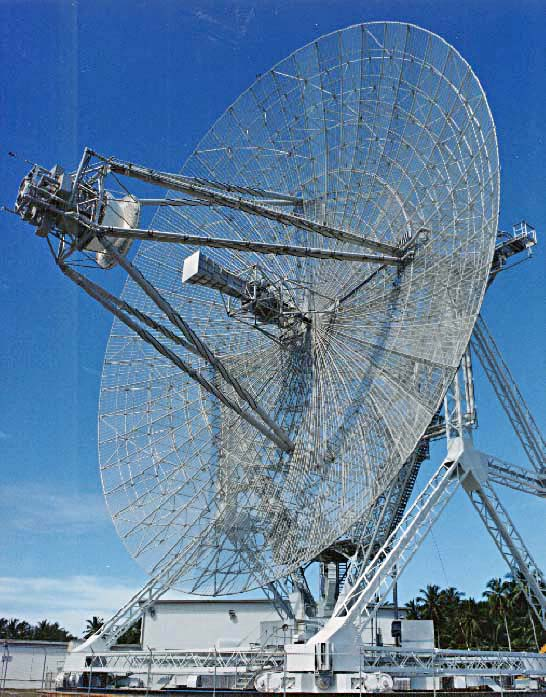
\includegraphics[width=0.9\textwidth]{Fixed_radar_antenna}
\caption{Fixed radar antenna}\label{fig:fixed_radar_antenna}
\end{minipage}\hfill
\begin{minipage}{0.3\textwidth}
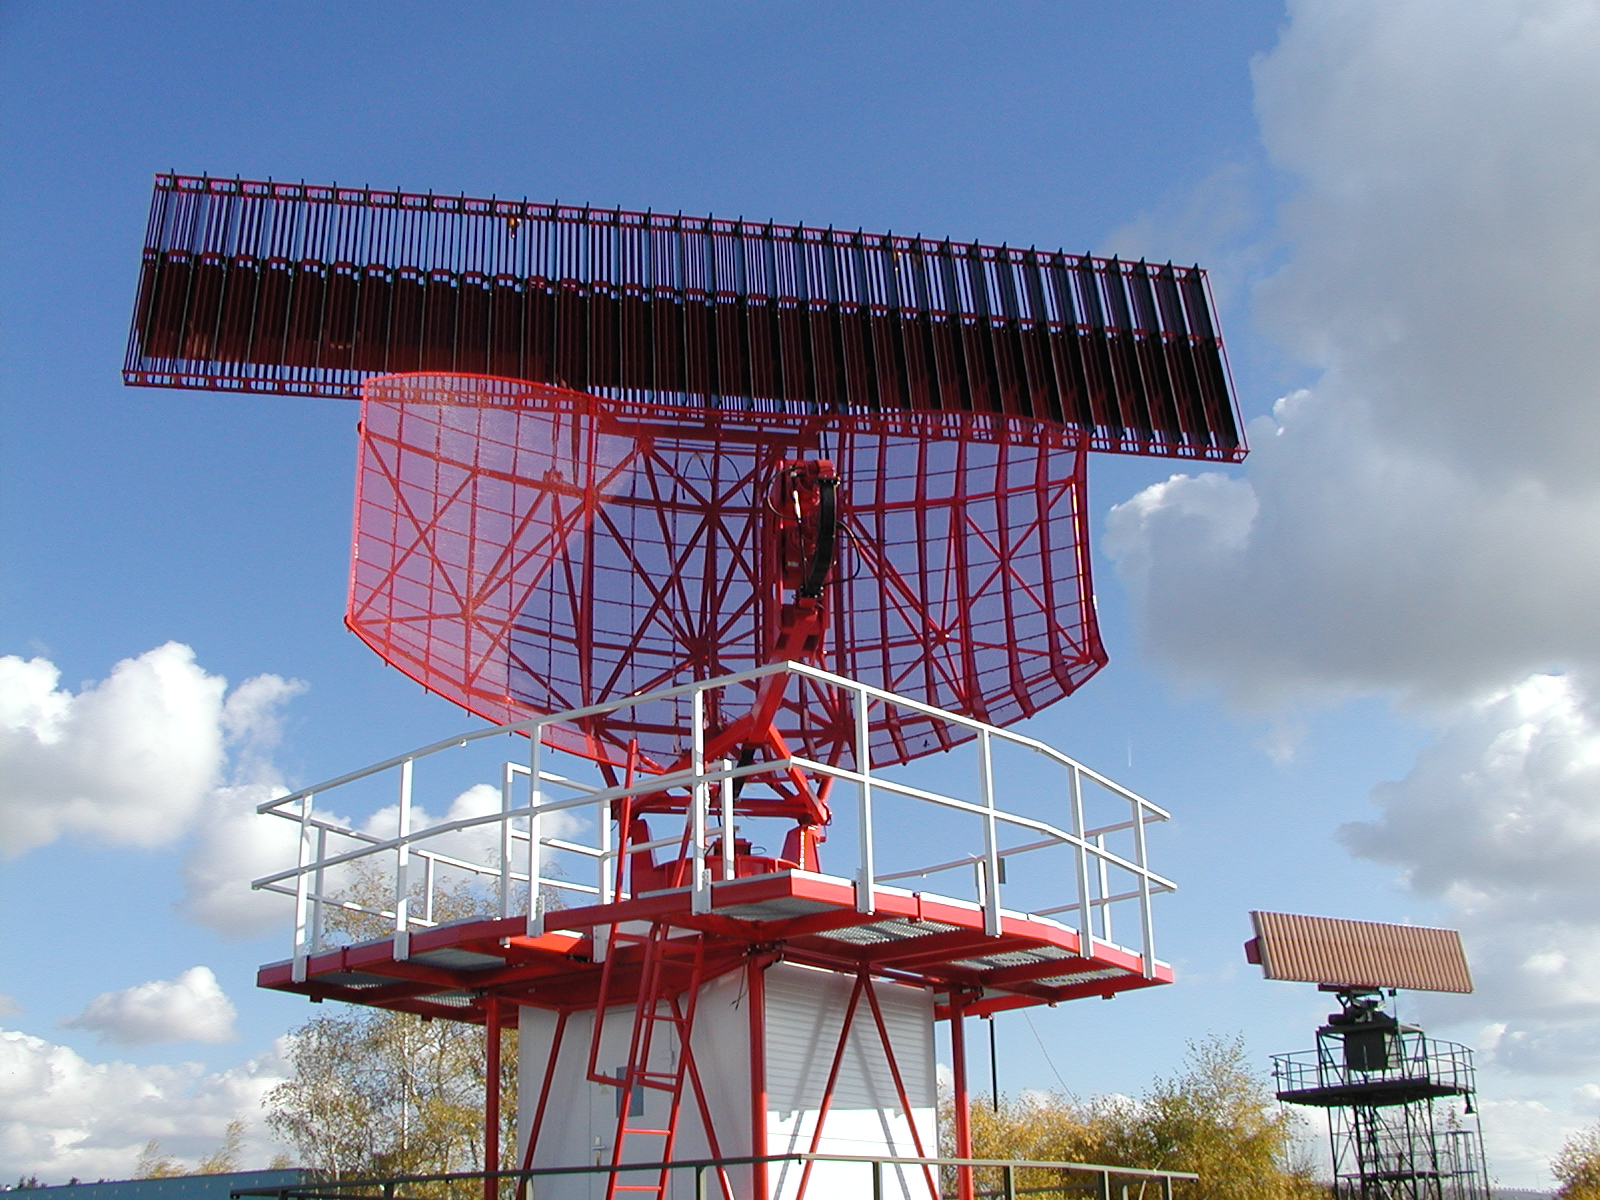
\includegraphics[width=0.9\textwidth]{Rotating_radar_antenna}
\caption{Rotating radar antenna}\label{fig:rotating_radar_antenna}
\end{minipage}\hfill
\begin{minipage}{0.3\textwidth}
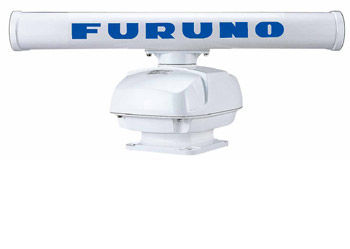
\includegraphics[width=0.9\textwidth]{Maritime_radar_antenna}
\caption{Maritime radar antenna}\label{fig:maritime_radar_antenna}
\end{minipage}
\end{figure}

\subsection{History}
The fist implementation of an instrument that were able to detect the presence of distance metallic objects by radio waves was done by Christian Hülsmeyer in 1904. His invention did not measure the distance to objects, but whether there was an object in the direction of the instrument. The radar as we know it today was introduced in the mid to late 1930's, with world war two triggering a research to improve the still immature technology to be used in military applications. After the war, the technology matured and where put in use in several civil applications, where air traffic control, maritime safety and weather monitoring is the most common.

\subsection{Principles}
The electromagnetic waves that a radar emits travels at the speed of light in air and vacuum. It reflects back when there is a change in the density of the medium it is travelling through, which is what happens when radio waves hit targets. Electrically conductive materials tends to be good reflectors, since they have a very different atomic density than air. On the other hand, materials with poor conductivity, and also some magnetic materials, then to absorb radio waves good. Like light, there is many ways an incoming radio wave can be reflected, primarily dependent on the geometry of the target. A corner with angles less than 180\degsym{} will reflect the incoming radio waves directly back to the sender, and is a good thing on targets that want to be visible on a radar. This principle are the basis for radar reflectors commonly used to boos the radar signature on smaller vessels, see Figure~\ref{fig:corner_reflector}.
\begin{wrapfigure}{R}{0.3\textwidth}
\centering
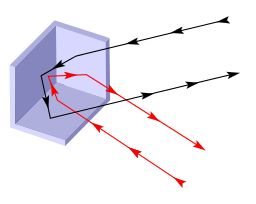
\includegraphics[width=0.25\textwidth]{Corner_reflector}
\caption{Corner reflector}\label{fig:corner_reflector}
\end{wrapfigure}
The opposite is used on targets that try to minimize their radar signature, and is the reason why stealth vessels and aircraft are tiled by flat areas. 
\begin{figure}
\centering
\begin{minipage}{0.3\textwidth}
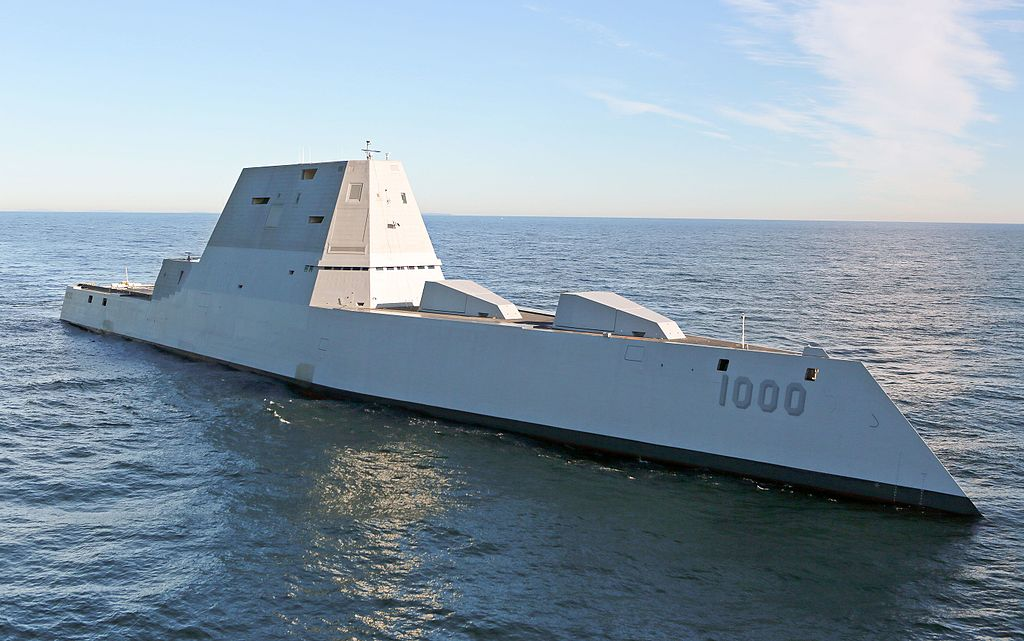
\includegraphics[width=0.9\textwidth]{USS_Zumwalt}
\caption{USS Zumwalt}\label{fig:uss_zumwalt}
\end{minipage}\hfill
\begin{minipage}{0.3\textwidth}
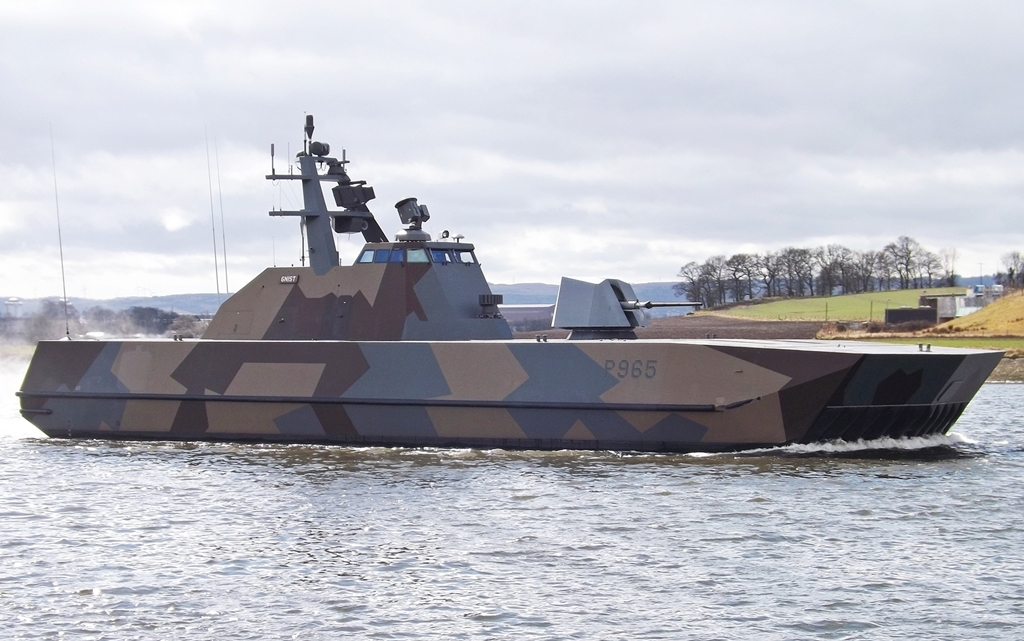
\includegraphics[width=0.9\textwidth]{KNM_Gnist}
\caption{KNM Gnist}\label{fig:knm_gnist}
\end{minipage}\hfill
\begin{minipage}{0.3\textwidth}
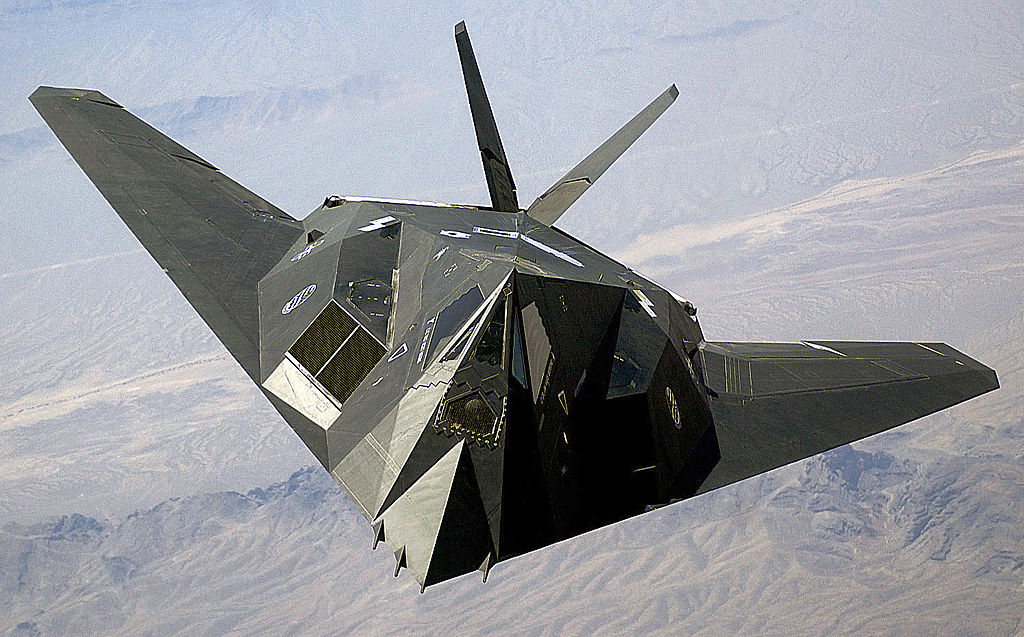
\includegraphics[width=0.9\textwidth]{Figures/F-117_Nighthawk}
\caption{F177 Nighthawk}\label{fig:f177_nighthawk}
\end{minipage}
\end{figure}

\section{AIS}
The \acrfull{ais} is a maritime safety and information system primarily designed for collision avoidance. \gls{ais} works by broadcasting messages on the \gls{vhf} band at irregular intervals with information on the vessels. \gls{ais} transceivers are required on international voyaging vessels over 300 \gls{gross_tonnage}, and on all passenger vessels. \gls{ais} signals are received at bother vessels and shore stations for use in \gls{vts} stations, open tracking databases like \url{www.marinetraffic.com}, fleet-monitoring and search and rescue. Since the \gls{ais} messages contains position, course and speed, \gls{ais} tracks can be overlaid on a map in a chart plotter or on top of a radar image, giving the operator two sensors to verify each other.

\subsection{History}
\gls{ais} was designed and developed by technical comities in the \gls{imo}. Its objective was to enhance vessels safety and efficiency by increasing their ability to see and identify other vessels. The main motivation for adopting \gls{ais} was its independence of humans in operation, since it automatically identifies other vessels and displays the information on the navigational system on the bridge. It also enables automatic calculation of \gls{cpa} and time until \gls{cpa}, in which the navigation system could alarm the bridge on incoming traffic on dangerous course. This gives the navigator on the bridge more and better information for making decisions, but with the caveat that not all vessels have \gls{ais}. In the 2002 \gls{imo} \gls{solas} Agreement, it is required that vessels over 300 \gls{gross_tonnage} and all passenger vessels must be equipped with class A AIS transceivers. A simpler and cheaper \gls{ais} version named class B aimed at smaller vessels and yachts was published in 2006, followed by a large increase in the amount of non-commercial vessels equipped with \gls{ais}.

\subsection{Messages}
\gls{ais} broadcasts both static, dynamic and voyage information with varying intervals based on the vessels speed, status and on request from shore stations. Static, dynamic and voyage messages are listed in Table~\cref{tab:static-ais,tab:dynamic-ais,tab:voyage-ais}. When the \gls{ais} standard was developed, the peak traffic situations in the two most densely trafficked waterways, Singapore and Dover Straits, where used to calculate the update frequency for the AIS system. Based on these two locations and a desire to keep the number of reports per minute below 2000, the dynamic information report intervals for class A and B was set as in Table~\ref{tab:classA_reporting_intervals} and~\ref{tab:classB_reporting_intervals} respectively~\cite{IALA2004}. Static information is transmitted every 6 minutes, and on request from \gls{vts} stations. \gls{ais} transceivers are utilizing two reserved \gls{vhf} channels; AIS 1 --- 87B (161.975MHz) and AIS 2 --- 88B (162.025MHz) to improve robustness against interference. An important note is that \gls{ais} transceivers are alternating which channel they are transmitting on, which means that if a receiver is only listening on one channel, the effective update rate halves.

\begin{table}
	\begin{tabularx}{\textwidth}{XX}
	\toprule
	\multicolumn{2}{c}{Static AIS information} \\
	\midrule
	MMSI & Maritime Mobile Service Identity \\
	Call sign & Maritime radio (VHF) call sign \\
	Name & Name of vessel \\
	IMO Number & Vessel IMO number \\
	Length and beam & \\
	Location of positioning fixing antenna & \\
	Height over keel & \\
	\bottomrule
	\end{tabularx}~\caption{Static AIS information}\label{tab:static-ais}

	\vspace{0.5 cm}

	\begin{tabularx}{\textwidth}{XX}
	\toprule
	\multicolumn{2}{c}{Dynamic AIS information} \\
	\midrule
	Position & In WGS84 frame \\
	Position accuracy & Better or worse that 10 meter \\
	Position time stamp & UTC in whole seconds \\
	Course over ground (COG) & \\
	Speed over ground (SOG) & \\
	Heading & \\
	Navigational status & \\
	Rate of turn (ROT) & \\
	\bottomrule
	\end{tabularx}~\caption{Dynamic AIS information}\label{tab:dynamic-ais}

	\vspace{0.5 cm}

	\begin{tabularx}{\textwidth}{XX}
	\toprule
	\multicolumn{2}{c}{Voyage AIS information} \\
	\midrule
	Draught & Depth in water \\
	Hazardous cargo & Type \\
	Destination & Name of place \\
	Estimated time of arrival (ETA) & \\
	Route plan / waypoints & \\
	Number of persons on board & \\
	\bottomrule
	\end{tabularx}~\caption{Voyage AIS information}\label{tab:voyage-ais}
\end{table}

\begin{table}
	\centering
	\begin{tabularx}{0.8\textwidth}{b s}
	\toprule
	Vessels status & Reporting Interval \\
	\midrule
	Ship at anchor or moored \newline and not moving faster than 3 knots & 3 minutes \\
	Ship at anchor or moored \newline and moving faster than 3 knots & 10 seconds \\
	Ship 0--14 knots & 10 seconds \\
	Ship 0--14 knots and changing course & 3.3 seconds \\
	Ship 14--23 knots & 6 seconds \\
	Ship 14--23 knots and changing course & 2 seconds \\
	Ship > 23 knots & 2 seconds \\
	Ship > 23 knots and changing course & 2 seconds \\
	\bottomrule
	\end{tabularx}~\caption{Class A Reporting Intervals}\label{tab:classA_reporting_intervals}

	\vspace{0.5 cm}

	\begin{tabularx}{0.8\textwidth}{b s}
	\toprule
	Vessels status & Reporting Interval \\
	\midrule
	Ship < 2 knots & 3 minutes \\
	Ship 2--14 knots & 30 seconds \\
	Ship 14--23 knots & 15 seconds \\
	Ship > 23 knots & 5 seconds \\
	Search and Rescue aircraft & 10 seconds \\
	Aids to navigation & 3 minutes \\
	AIS base station & 10 seconds \\
	\bottomrule
	\end{tabularx}~\caption{Class B Reporting Intervals}\label{tab:classB_reporting_intervals}

\end{table}

\subsection{Class A}
Class A \gls{ais} transceivers are designed for \gls{sotdma} transmission, which is a way of reserving transmission time slot for the next broadcast. \gls{sotdma} is based on \gls{tdma}, with an extension allowing for self organizing of time slots compared to \glspl{tdma} dedicated timing manager. This effectively gives class A AIS transmissions priority over Class B equipment which may not have \gls{sotdma}. Class A transceivers are also required to have build-in display, minimum transmission power of 12.5W, ability to filter targets and communication interfaces like \gls{rs232} and \gls{nmea}.

\subsection{Class B}
Class B \gls{ais} transceivers are designed to be simpler and cheaper than Class A transceivers, which is accomplished through less strict requirements for hardware and operation. Class B \gls{ais} transmits at lower power, usually 2W and transmits at larger time intervals than Class A, see Table~\ref{tab:classB_reporting_intervals}. It is not required to have a build-in display and can use both \gls{cstdma} and \gls{sotdma} for transmission. \gls{cstdma} is a simpler approach to time division than \gls{sotdma} since it only listen for a single time slot to be unused before it transmits.

\section{Tracking}
\subsection{Overview}
Tracking, in this context, is the process of estimating the state of stationary and moving targets that are observed by a system without included association data. The challenge is to know which measurements belong together over time, often refereed to as the data association problem. An observation system can be a radar, sonar or any other sensor that, passively or actively, detects objects within an area or volume. Any observation system will be prone to noise, both in form of internal- and external noise from the environment. This noise will cause false measurements that the tracking system must take care of. These false measurements are often referred to as clutter.

In this work `tracking algorithm' will be used to describe the main logic in a tracking method or approach, while `tracking system' will be used on complete systems with everything around the main algorithm included. A tracking system can be defined as: \emph{A system that process consecutive measurements from one or more observation system and associates measurement from the same target into tracks with initialization of new tracks and termination of dead tracks}. A track is a sequence of states associated with a subset of all measurements from the observation systems. 

Tracking is a relative new filed of study, driven by the military and aerospace industry and enabled by the development of microprocessors and computers from the 1960's. The applications ranges from sonar tracking on both submarines and navy vessels, to air control and missile guidance. This historical background is likely the reason for most published papers using these types of applications as background for testing. In recent years, tracking people and vehicles from visual- and \gls{sar} imagery have also become a topic in the research community~\cite{Carthel2007,Carthel2007a,Coraluppi2000}. New applications areas like oceanography, autonomous vehicles and biomedical research have also found use of tracking~\cite{Wolf2010,Svec2014,Vo2015}.

There are several factors contributing to the challenge of good tracking; \gls{clutter}, lower than unity \gls{Pd}, multiple detections of the same vessel and wakes. \Gls{clutter} is a term for unwanted measurements or noise, which is inherent in every observation system. For a maritime radar, this can be caused by waves, rain, snow, birds or shore echo. A common assumption on clutter is to assume the amount being Poisson distributed, and spatially uniformly distributed. \gls{Pd} is a measure of how persistent the target is in the measurements, and will vary much between different types of targets, primarily dependent on their size, construction material and shape. Multiple detections of each target can occur when the target is large and have several distinct areas which reflects radar waves better than the rest of the vessel, for instance when the hull of a boat is made from fibreglass and the metal objects inside is reflecting. Wakes are reflection caused by the turbulent water behind a moving object, which can be a problem for both sonar and maritime- and air-radar.

\subsection{Single-target tracking}
The simplest approach to tracking is single-target tracking, where it is assumed that there are only one target in the measurement area, and any other measurement is regarded as either extra measurements of the target or \gls{clutter}. 

\subsubsection*{\gls{nnf}}
The simplest single-target tracking algorithm is the \gls{nnf}, where the closest measurement is always selected~\cite{Bar-Shalom1998}. This approach is very vulnerable to clutter and dense multitarget scenarios, which is probably the reason its usage is very sparse. 

\subsubsection*{\gls{pdaf}}
The arguably best single-target tracking algorithm is \gls{pdaf}, which calculates probabilities of all target to measurement association for all measurement inside its gate. A gate is an ellipse (2D) or ellipsoid (3D) which outlines the confidence area / volume for a predicted state and covariance for a given confidence value. The state update is then based on a weighted sum of measurement innovations where the weightings are the probabilities for their respective innovations. One of the main assumptions in \gls{pdaf} is that all the measurements inside its gate contains information about the targets true state. This assumption performs well in single-target scenarios since targets often create more than measurements, and thus using all measurements in state estimation effectively rejects much of the \gls{clutter} in each \gls{scan}.

\subsection{Multitarget tracking}
A more generalized approach assuming that there can be any number of targets is called multitarget tracking. The problem expands to jointly estimate both the number of targets and their trajectories since targets can enter and leave the surveillance area. 

While a large number of tracking techniques have been developed, the three most used are \gls{jpdaf}, \gls{mht} and \gls{rfs}~\cite{Vo2015}. Compared to \gls{mht} and \gls{jpdaf}, \gls{rfs} is a relatively new approach to tracking, and is not  matured the same way \gls{mht} and \gls{jpdaf} are. \gls{mht} and \gls{jpdaf} also differs from \gls{rfs} in that they both do data association and filtering, whereas \gls{rfs} directly seeks both optimal and suboptimal estimates of the multitarget state~\cite{Vo2015}.

\subsubsection{JPDAF}
\gls{jpdaf} is a multitarget expansion of \gls{pdaf} which is a single-target tracking technique. PDAF calculates joint posteriori association probabilities for every target in every scan. Each targets probability is a weighted sum of probabilities, where the weights are the key difference between \gls{pdaf} and \gls{jpdaf}. Like \gls{mht}, \gls{jpdaf} suffers from high computational cost, and an efficient implementation approach exist and is patented by QinetiQ~\cite{Horridge}.

\subsubsection{MHT}
\gls{mht} is a decision logic which generates and maintains alternative hypotheses when new \glspl{measurement} are received and within the gate. By making several possible hypotheses, the decision on which \gls{measurement} to choose can be propagated into the future when more information is available. MHT is multi frame method, meaning it has the ability to utilize multiple scans to make better decisions. Each hypothesis is given a \gls{score} based on a likelihood ratio as a reflection of how well the measurement fits the model, which are accumulated to evaluate the combinations of consecutive \glspl{measurement}.

In contrast to the \gls{pdaf} and \gls{jpdaf} methods who suffers from track \gls{coalescence}, \gls{mht} methods split when in doubt. The idea of using multiple hypotheses was first introduced by~\cite{Singer1974}, but the first complete algorithm was presented in~\cite{Reid1979}, where a \gls{homht} was developed. Following this, a \gls{tomht} was proposed in~\cite{Kurien1990} and the \gls{score} function for \gls{mht} was later deduced and discussed in~\cite{Bar-Shalom2007} since no explicit track-score function were given in~\cite{Kurien1990}. \gls{mht} is, in the same way as \gls{pdaf}/\gls{jpdaf}, developed under two main assumptions; that at most one \gls{measurement} can originate from each \gls{target} in each scan, and that a \gls{target} does not necessarily show on every scan, or in other words, \gls{Pd} less than 1. The \gls{mht} approach to tracking and data association was for a long time dismissed by many because of its computationally large cost. The dramatic increase in computational capability from the 1980's to the late 2010's have, however, lead to a new spring for \gls{mht}, with an increasing interest for use in tracking system. In 2004 Blackman stated that \say{Multiple hypothesis tracking is generally accepted as the preferred method for solving the data association problem in modern multiple \gls{target} tracking system}~\cite{Blackman2004}. Already in 2001 did Blackman publish a demonstration that \gls{mht} is capable of real-time demands~\cite{Blackman2001}.

\gls{mht} comes in two variations, \gls{homht} and \gls{tomht}. They differ in their approach to arrange the measurements into hypotheses in that \gls{homht} builds hypotheses that are different ways of organizing the measurements into tracks, while \gls{tomht} maintains already existing tracks and a hypothesis is only a possible track for a single target and not all targets. This means that in \gls{tomht}, to select the 


\subsubsection{\gls{rfs}}
\Gls{rfs} is a family of Bayesian methods and filters that is based on representing a multitarget state as a finite set of single target states. By not having the multitarget states represented as a vector, the estimation error is more meaningful and mathematically consistent. This is because the vector representation is ordered, and thus the only meaningful way of representing the estimation error would be to minimize the estimation error over all permutations of states. This can be represented as distances between finite sets, and is a much more well defined and understood concept. 
% \Gls{rfs} method are, like \gls{pdaf} and \gls{jpdaf}, based on representing the history of a target as a prior probability density.

The \gls{rfs} approach to multi sensor multitarget tracking was done by Mahler in 1994, which lay the foundation for the development of \gls{fisst}. One popular filter based on \gls{rfs} is the \gls{phd} filter. The \gls{phd} filter is an approximation of the multitarget Bayes filter derived by Mahler using \gls{fisst}~\cite{Vo2015}. The \gls{phd} filter estimates the number of targets and then selects the same numbers highest probable tracks. One large drawback with the \gls{phd} filter is its assumption that the predicted multitarget \gls{rfs} is Poisson distributed. This assumption is relaxed in the \gls{cphd} filter where the prior and predicted multitarget densities are independently and identically distributed clusters. \clearpage 
	%!TEX root = ../TTK4900-MHT.tex

\chapter{Radar and AIS preprocessing}\label{chapter:radar-and-ais-preprocessing}
The process from raw radar and \gls{ais} data to target tracks is made up from several processing steps. The aim of this chapter is to give the reader a basic understanding of these steps and their challenges.

\section{Radar preprocessing}
Rotating maritime radars (Figure~\ref{fig:maritime_radar_antenna}) are wide and short, giving them a tall and narrow beam. A ping transmit and receive sequence is carried out for each antenna rotation angle in the radars scan resolution. This gives reflections as signal level in spokes described by polar coordinates, rotation angle and distance. Each spoke has a width determined by the design of the antenna, primarily the width of the antenna, and a number of cells dictated by the discretization and sampling interval of each spoke. The spokes is then run through a detection algorithm, which is filtering adjusting the received signal according to detection setting. The detection algorithm is often built in to the radar system, with both fixed and user adjustable detection parameters.

When displayed on a screen in a vessels, the output from the detection step is viewed and interpreted by the operators. In an automated scenario with autonomous vessels, the next step would be to transform the detections from polar vessel body frame to for instance a Cartesian world fixed local frame. Which frame to convert two is a design choice, and can be dependent on use-case, interconnected systems and performance requirements. This transformation is strongly dependent on knowing the position and attitude of the vessel at each spoke sampling time, which is fed from the vessels navigation system.

With all the spoke resolution cells converted to a world-fixed Cartesian coordinate system, it is desirable to remove land reflections if any. This step is dependent on highly detailed digital maps of the area in question, and is commercially available for most of the world. Since maps have both offsets and inaccuracies to some extent, a cleaner land masking can be accomplished by dilating the coastline. This is in may situations acceptable since the vessels will never be that close to shore, and any targets masked away is in a region out of interest.

The last step in the radar processing chain is to convert a point cloud into measurements, as one target will in most cases fill multiple resolution cells and therefore it does not yield good result to send all cells with detection forward as measurements. This clustering of the detections also need to take into consideration the assumption that each target maximum generates one measurements. This leads to clustering algorithms that assumes that detections closely spaced are originating from the same target, and thus should be one measurement. There is many clustering algorithms available to solve this problem, some builds graphs with vertices between neighbouring detections given a neighbour criterion, some estimates the number of clusters and optimizing the detections into this number of clusters~\cite{Mahmuddin2010,Pelleg2000}. When a set of detections are clustered, their respective measurement is calculated as the centroid of the detections, which would be weighted by their signal strength if available. These measurements are sent to the tracking module.

\subsection{Frame conversion}\label{subsec:frame_conversion}
The radar measurements is by nature in polar frame, and the target motion model is best described in a Cartesian frame. The most usual solution is to convert the radar measurements to a Cartesian frame, and to avoid biased and optimistic covariances of the converted measurements, a procedure which compensates for these errors, (\ref{eq:debiased_coordinate_conversion}) and (\ref{eq:average_true_converted_measurement_covariace}),  should be used in stead of the standard conversion (\ref{eq:standard_coordinate_conversion}) and (\ref{eq:linearized_converted_measurement_covariace})~\cite{Bar-Shalom1995}.
\begin{equation}\label{eq:debiased_coordinate_conversion}
\begin{split}
\begin{bmatrix} x \\ y \end{bmatrix} &= \begin{bmatrix} r_m \cos \theta_m  \\ r_m \sin \theta_m  \end{bmatrix} - \mu_a \\
\mu_a & \triangleq 
\begin{bmatrix}
	E \lbrack \tilde{x}|r_m,\theta_m \rbrack \\ 
	E \lbrack \tilde{y}|r_m,\theta_m \rbrack 
\end{bmatrix} 
= 
\begin{bmatrix}
	r_m \cos \theta_m (e^{-\sigma^2_\theta}) - e^{-\sigma^2_\theta / 2} \\ 
	r_m \sin \theta_m (e^{-\sigma^2_\theta}) - e^{-\sigma^2_\theta / 2}
\end{bmatrix} 
\end{split}
\end{equation}

\begin{equation}\label{eq:average_true_converted_measurement_covariace}
\begin{split}
R_a^{11} & \triangleq r_m^2 e^{-2\sigma_\theta^2} \lbrack \cos^2\theta_m(\cosh 2\sigma_\theta^2-\cosh \sigma_\theta^2) + \sin^2\theta_m (\sinh 2\sigma_\theta^2 - \sinh \sigma_\theta^2) \rbrack \\
& + \sigma_r^2 e^{-2\sigma_\theta^2} \lbrack \cos^2 \theta_m (2\cosh 2\sigma_\theta^2 - \cosh\sigma_\theta^2) + \sin^2 \theta_m (2\sinh 2\sigma_\theta^2 - \sinh \sigma_\theta^2) \rbrack \\
R_a^{22} & \triangleq r_m^2 e^{-2\sigma_\theta^2} \lbrack \sin^2\theta_m(\cosh 2\sigma_\theta^2-\cosh \sigma_\theta^2) + \cos^2\theta_m (\sinh 2\sigma_\theta^2 - \sinh \sigma_\theta^2) \rbrack \\
& + \sigma_r^2 e^{-2\sigma_\theta^2} \lbrack \sin^2 \theta_m (2\cosh 2\sigma_\theta^2 - \cosh\sigma_\theta^2) + \cos^2 \theta_m (2\sinh 2\sigma_\theta^2 - \sinh \sigma_\theta^2) \rbrack \\
R_a^{12} & \triangleq \sin \theta_m \cos \theta_m e^{-4\sigma_\theta^2} \lbrack \sigma_r^2 + (r_m^2 + \sigma_r^2)(1-e^{\sigma_\theta^2}) \rbrack
\end{split}
\end{equation}

\begin{equation}\label{eq:standard_coordinate_conversion}
x = r_m \cos \theta_m \qquad y = r_m \sin \theta_m
\end{equation}

\begin{equation}\label{eq:linearized_converted_measurement_covariace}
\begin{split}
R_L^{11} & \triangleq r_m^2 \sigma_\theta^2 \sin^2\theta_m + \sigma_r^2 \cos^2 \theta_m \\
R_L^{22} & \triangleq r_m^2 \sigma_\theta^2 \cos^2\theta_m + \sigma_r^2 \sin^2 \theta_m \\
R_L^{12} & \triangleq (\sigma_r^2 - r_m^2 \sigma_\theta^2) \sin \theta_m \cos \theta_m \\
\end{split}
\end{equation}

\begin{equation*}
\begin{split}
r_m 			&= \text{measured range} \\
\theta_m		&= \text{measured bearing} \\
\sigma_r 		&= \text{range measurement standard deviation} \\
\sigma_\theta 	&= \text{bearing measurement standard deviation} \\
\M{R_a} 		&= \text{average true converted measurement covariance} \\
\M{R_L} 		&= \text{linearised converted measurement covariance} \\
\end{split}
\end{equation*}

\section{AIS preprocessing}~\label{sec:ais_preprocessing}
\Gls{ais} does not suffer from the association uncertainty, clutter and low accuracy like radar measurement. It does however have some issues caused by suboptimal or erroneous transmitter implementation, transmission collision caused by \gls{tdma} leading to ID (\gls{mmsi}) swaps, and delayed messages leading to out of order reception. In order to remove most of these errors, it is desirable to filter the incoming \gls{ais} messages before sending them to the tracking module.

\subsection{Out-of-order filtering}
All \gls{ais} messages are stamped with the \gls{utc} of transmission, and `frequently arrive out-of-order'~\cite{Wilthil}, illustrated in Figure~\ref{fig:out_of_order_ais} stolen from~\cite{Wilthil}.
%Stjålet hardt og brutalt
\begin{figure}[H]
\centering
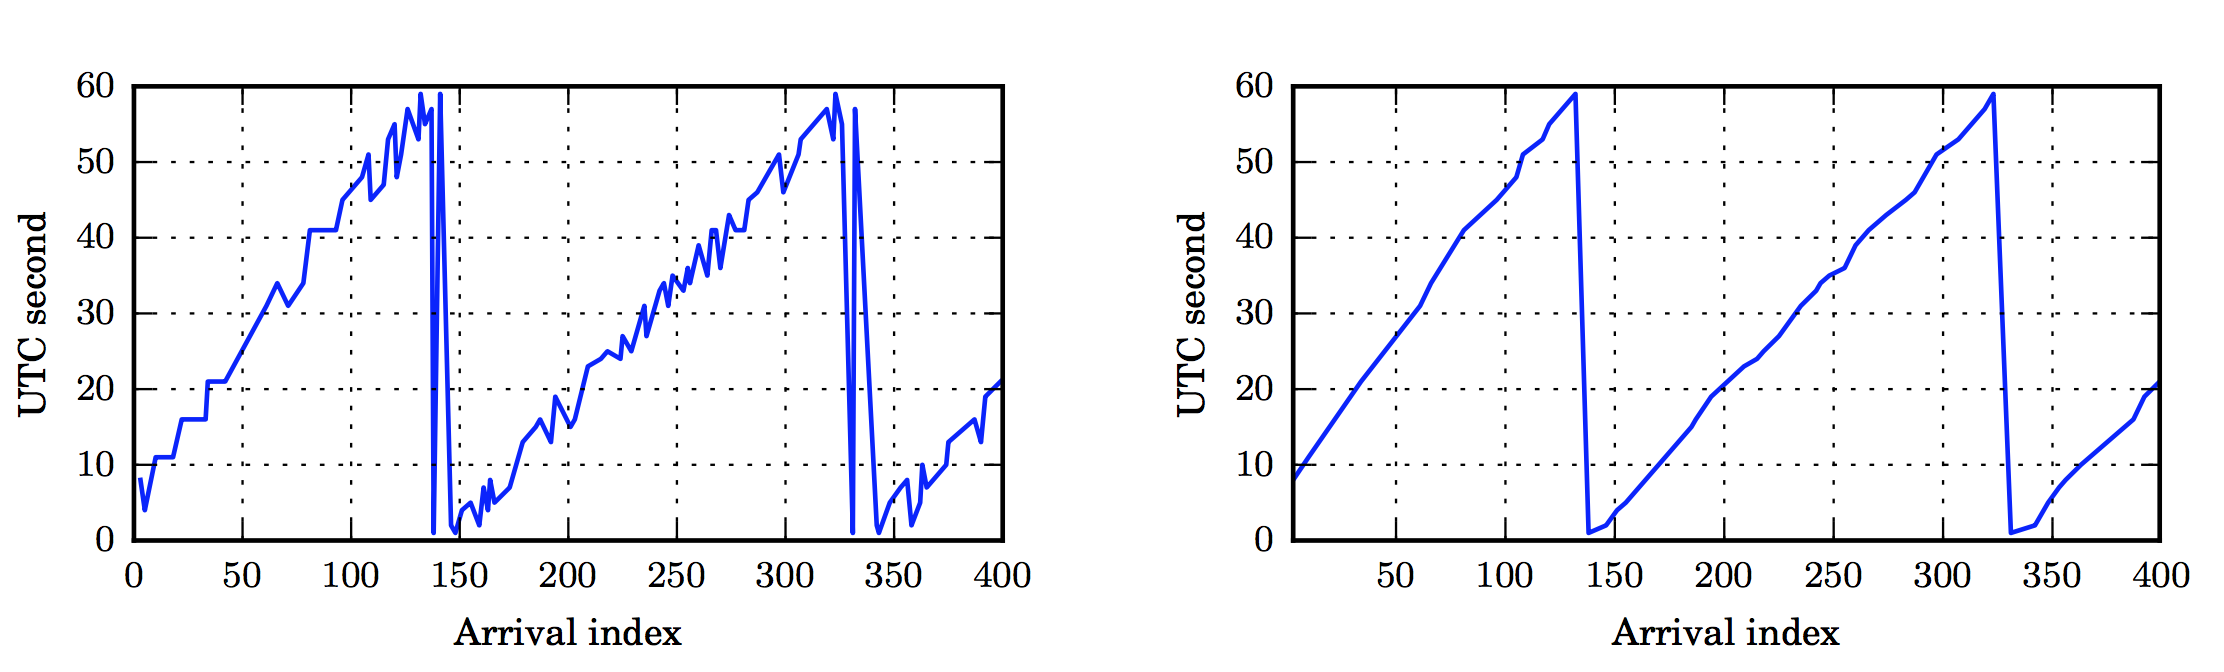
\includegraphics[width = .9\textwidth]{Figures/out_of_order_ais.png}
\caption{Unfiltered and filtered AIS arrival time~\cite{Wilthil}}\label{fig:out_of_order_ais}
\end{figure}
One of the simplest ways of remedying this issue is to discard all messages with older timestamps that the current newest for each \gls{mmsi}. This will lead to a loss of data, which will lead to a slower AIS update period for the tracking module.

\subsection{ID swap filtering}
According to~\cite{Harati-Mokhtari2007}, 2\% of the received AIS messages in a data-mining study contained erroneous ID or \gls{mmsi}. One of the errors where that many vessels transmitted messages with the same MMSI (11930446). This is the default MMSI on equipment from a specific manufacturer. Another example is two vessels which swapped IDs for a moment when they were passing, with a recovery after about 15 minutes. The latest example could be caused by simultaneous transmission or reflections, but the cause is not examined in the paper. Although much rare that the out-of-order reception   

To remedy this issue, a simple test logic can be incorporated to check for obvious faults like sudden large position change and known default IDs. When a message and MMSI is categorized as bad, it would be held back from the tracking module. 

\subsection{Synchronization}
Since AIS messages arrive asynchronously and the tracking module is only accepting AIS updates along with radar updates, we must synchronize the incoming AIS messages. In this work, all \gls{ais} measurements are buffered from when they are received until the next radar scan and predicted according to the tracking modules motion model forward in time to match the radar scan time. This is a design choice, which in some sense synchronize the AIS to the radar. Since the radar period is much smaller than (or in the best case for the AIS, equal to) the AIS transmit period, this will seldom lead to unused AIS measurements. On the other hand, since the radar period is relative short, the amount of time any AIS position will be predicted forward is typically small enough to not cause uncertainty larger than manageable for the algorithm.

As will be clear in Section~\ref{subsec:combined_radar_and_ais_hypotheses}, this prediction is only used for the gating sequence.

 \clearpage
	%!TEX root = ../TTK4900-MHT.tex

\chapter{MHT Module}\label{chapter:mht-module}
To create a complete tracking \emph{system}, rather than a tracking \emph{\gls{algorithm}}, it is often necessary to complement the main algorithm with support modules. The system, or module if it is a part of a bigger system, presented here is an extension of the pre master project~\cite{Liland_2017}. The aim of this chapter is to provide a complete walkthrough of the the track oriented MHT system developed in this thesis. This \gls{mht} module is based on both radar and \gls{ais} data from sensors mounted on own vessel. Since the radar is one of the most trustworthy sensors on board any vessel is this tracking module based on radar measurement primarily, with the \gls{ais} as an aiding system. This approach guided some of the design choices made throughout the development of the module. 

The motion model which is used throughout the entire tracking system when predicting and filtering target behaviour is presented first. Next follows an overview of the algorithm used to initiate new tracks into the MHT algorithm, followed by the entire MHT tracking algorithm with all its sub-routines.

It will be assumed throughout this thesis that radar data is processed, as outlined in Section~\ref{sec:radar_preprocessing}, into a set of points. These points is referred to as radar measurements.

\section{Motion Model}\label{sec:motion-model}
\subsection{Reference frame}
A local Cartesian NED-frame, like \gls{utm} will be used throughout this thesis, with the assumption than all input sensors are transformed to this frame (see Section~\ref{subsec:frame_conversion}). This local projection from a geodetic coordinate system to a Cartesian coordinate system is acceptable as long as the the area the system is working on is within one grid. A global geodetic frame, like WGS84 would be preferable in situations where the system tracks object over world-scale lengths but would yield non-linear equations of motion.

\subsection{Constant velocity model}
A target's state (\ref{eq:state_vector}) is modelled with position and velocity in a 2D Cartesian frame where the positive \(x\)-axis is pointing east and the positive \(y\)-axis is pointing north. The two latest states are the velocities in their respective direction.
\begin{equation}
\V{x} = \begin{bmatrix}
x & y & \dot{x} & \dot{y}
\end{bmatrix}^T
\label{eq:state_vector}
\end{equation}

Since modelling the behaviour of any ship under unknown command is next to impossible, a common assumption in tracking theory is that every target will continue on as usual, more precisely that their velocity is constant. Although simple, this model captures the essence of most vessels at sea, and it should be noted that both maritime training~\cite{Allen2005} and regulation~\cite{IMO1972} dictates that vessels should hold steady course and change course in clear decisive turns. This model is also very common in tracking applications and is used in~\cite{Reid1979,Coraluppi2000,Brekke2012,Wilthil,Vo2015,Chen2003,Habtemariam2015} among others. To give room in our model for manoeuvring, process noise is introduced with covariance set according to the assumed manoeuvring capabilities of the vessels. This could be set as a fixed value for all targets, as done in this work, or estimated based on the history of the track or AIS information. This behaviour can be modelled as a linear time invariant system with time evolution (\ref{eq:motion_model}), measurement model (\ref{eq:measurement_model}), transition and observation matrices (\ref{eq:model_matrices}), and system and measurement noise matrices (\ref{eq:noise_matrices}).

\begin{equation}\label{eq:motion_model}
\V{x}_{k+1} = \M{\Phi} \V{x}_k + \V{w}_k \qquad \V{w} \sim \mathcal{N}(0;\M{Q})
\end{equation}
\begin{equation}\label{eq:measurement_model}
\V{z}_{k+1} = \M{H}\V{x}_k + \V{v}_k \qquad \V{v} \sim \mathcal{N}(0;\M{R})
\end{equation}
\begin{equation}\label{eq:model_matrices}
\M{\Phi} =	\begin{bmatrix}
1 & 0 & T & 0 \\
0 & 1 & 0 & T \\
0 & 0 & 1 & 0 \\
0 & 0 & 0 & 1 \\
\end{bmatrix}
\quad
\M{H} =	\begin{bmatrix}
1 & 0 & 0 & 0 \\
0 & 1 & 0 & 0 \\
\end{bmatrix}
\end{equation}
\begin{equation}\label{eq:noise_matrices}
\M{Q}	= \sigma_v^2 \begin{bmatrix}
\frac{T^3}{3} 	& 0 				& \frac{T^2}{2}	& 0 			\\
0 				& \frac{T^3}{3}  	& 0 			& \frac{T^2}{2}	\\
\frac{T^2}{2}	& 0					& T				& 0				\\
0				& \frac{T^2}{2}		& 0				& T				\\
\end{bmatrix}
\quad
\M{R} =	\sigma_m^2 
\begin{bmatrix}
1 & 0 \\
0 & 1 \\
\end{bmatrix}
\end{equation}
\begin{equation*}
\begin{split}
\M{\Phi} 	&= \text{state transition matrix} \\
\M{H}		&= \text{state observation matrix} \\
\M{Q}		&= \text{system covariance matrix} \\
\V{w}		&= \text{\gls{system noise}} \\
\V{v}		&= \text{\gls{measurement noise}} \\
\V{z}		&= \text{measurement vector} \\
k 			&= \text{time index} \\
T  			&= \text{time step} \\
\end{split}
\end{equation*}

\section{Track Initiation}
In comparison with \gls{homht}, which treats every measurement as a potential new track. \Gls{tomht} does not have any built-in initialization of tracks since it only maintains already existing tracks with track splitting and measurement-to-track association for every scan. To remedy this lack, we need an algorithm that can find consistent and predictable patterns in an assumed uniformly distributed measurement space of clutter. 

In this work, new tracks are initiated with 2/2 \& m/n logic~\cite{Vo2015} on the unused measurements after each MHT iteration. As the name of the method indicates, this is a two step verification, where the first act as a rough filter and the second as a fine filter. As a common in most tracking systems, the radar clutter is assumed uniformly distributed in the measurement area. 
%This assumption is quite rough in the radial measurement space, and even worse approximation in Cartesian measurement space, as illustrated in \Cref{fig:clutter_radial,fig:clutter_cartesian}.  Although far from perfect, tests shows that we still get satisfactory performance from the 2/2\&m/n method.
% \begin{figure}[H]
% \centering
% \begin{minipage}{0.45\textwidth}
% 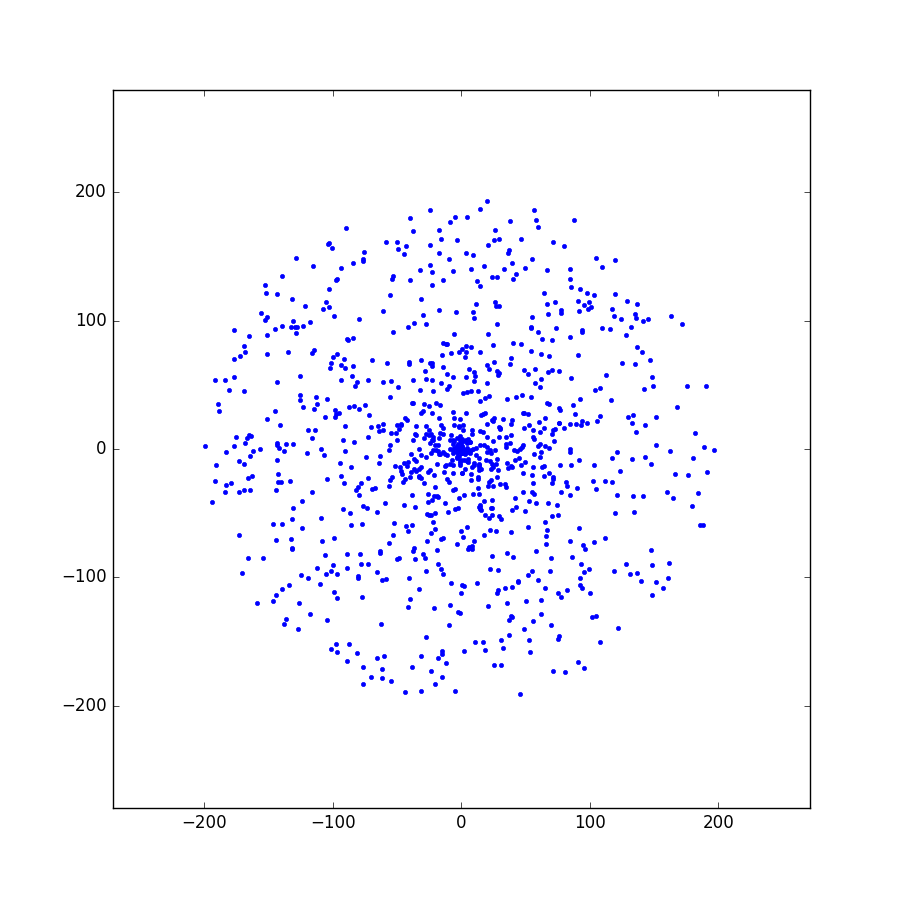
\includegraphics[width=\textwidth]{Figures/clutterRadial.png}
% \caption{Uniform radial clutter}\label{fig:clutter_radial}
% \end{minipage}\hfill
% \begin{minipage}{0.45\textwidth}
% 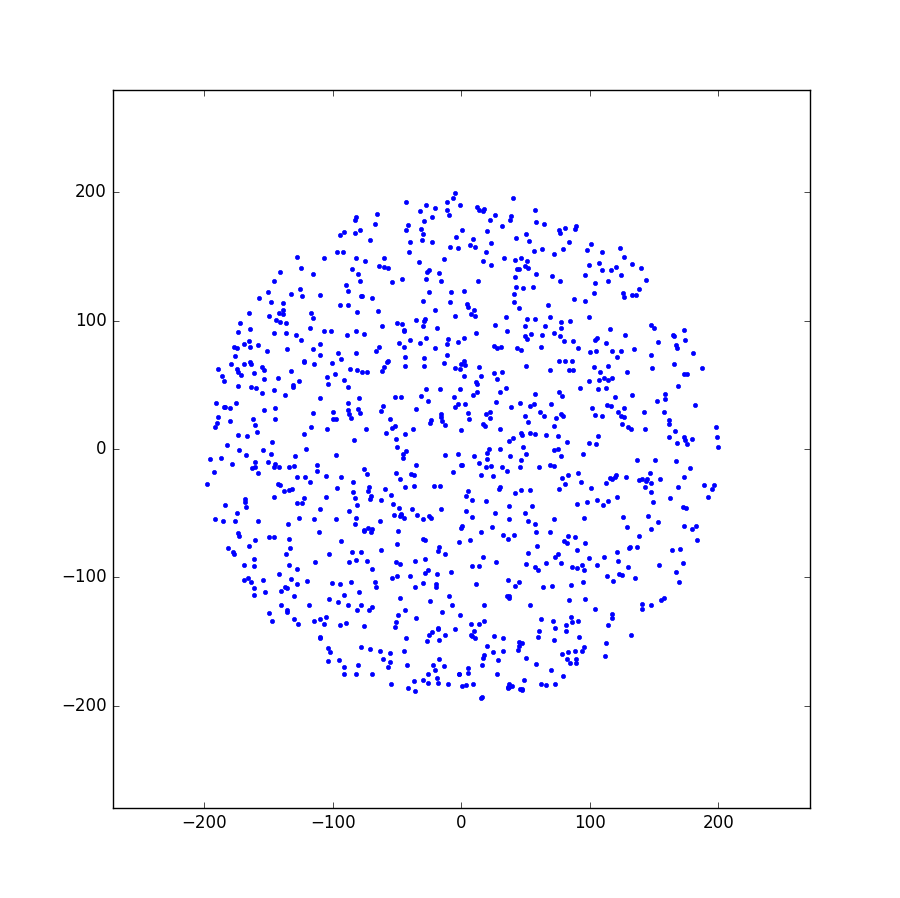
\includegraphics[width=\textwidth]{Figures/clutterCartesian.png}
% \caption{Uniform Cartesian clutter}\label{fig:clutter_cartesian}
% \end{minipage}
% \end{figure}

The flow of the method is illustrated in Figure~\ref{fig:init_flowchart}, and for better clarity, the algorithm is explained from the last step to the first step, since this is the sequence a newly started initiation algorithm will perform its operations.
\begin{figure}[H]
\centering
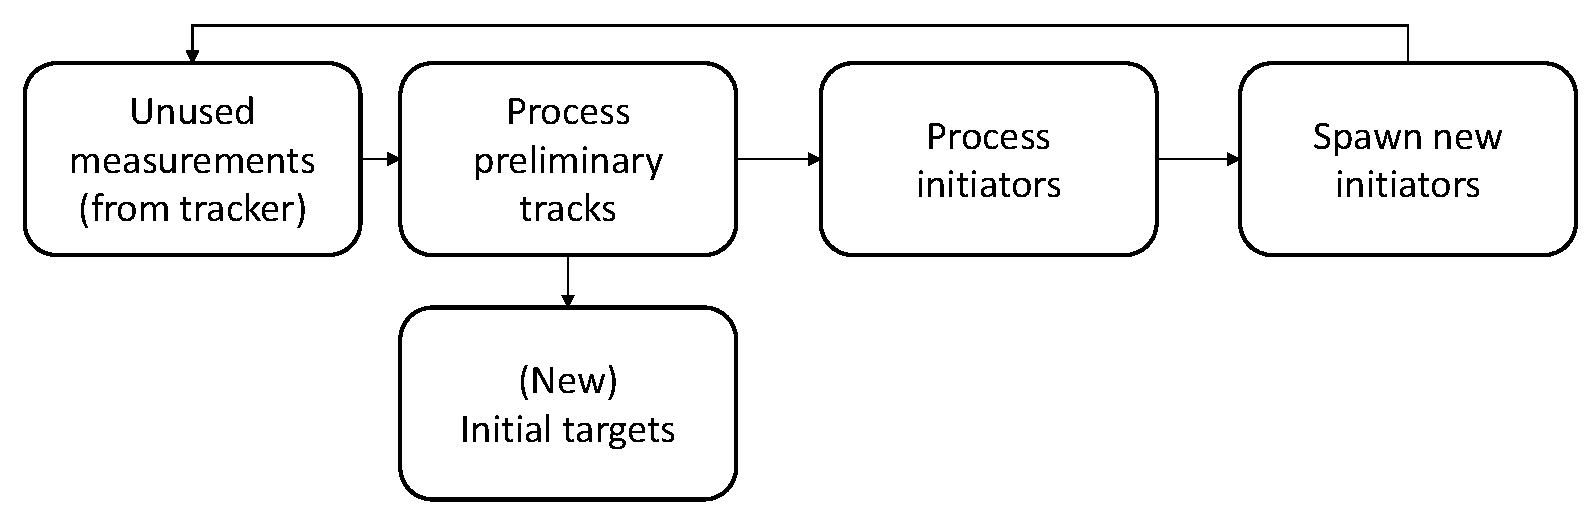
\includegraphics[width = .9\textwidth]{init_flowchart.pdf}
\caption{2/2\&m/n flowchart}\label{fig:init_flowchart}
\end{figure}

\subsection{Spawn new initiators}
All measurement unused by the `Process preliminary tracks' and `Process initiators' steps will be the basis for new \emph{initiators}. An initiator is a measurement that awaits its match in the next scan. The idea is that uniformly distributed clutter will not (often) reappear at approximately the same location two times in a row, effectively filtering out most of the clutter.

\subsection{Process initiators}
When the next scan arrives, all the unused measurements from the `Process preliminary tracks' step will be used as candidates in this step. Since an initiator is only a position and not a full state with velocity, all directions are equally likely, and the only design parameter in this step is maximum speed of targets to be tracked. This parameter sets an outer limit on the circle acting as a gate for the second and confirming measurement. When matching initiators with a second measurement, we want to select the closest measurement, making the assumption that the two consecutive measurements are the most likely to belong together. In a single target scenario, where this would be to calculate the distance to all the alternative measurements and select the lowest, the association is already done. While in a multitarget scenario, we \emph{could} select the closest measurement to any initiator, but we would have to do this one initiator at a time. This would lead to different results depending on the arrangement of the initiators in the programming of this method. A different approach would be to calculate all the different distances for any possible combination of initiators and measurements, sort the list, and assign the distances from the shortest to the longest possible distances. This approach would not be influenced by randomness like the arrangement of the initiators in a programming language, but would not necessarily give the global optimal association regarding the how many initiators that are assigned measurements and their respective distances.

Since we can have situations like exemplified in Figure~\ref{fig:init_gating}, where two initiators have the same measurement inside their gates, and one of them have a second measurement inside its gate, we need to take the global consequence of any assignment into consideration.
\begin{figure}
\centering
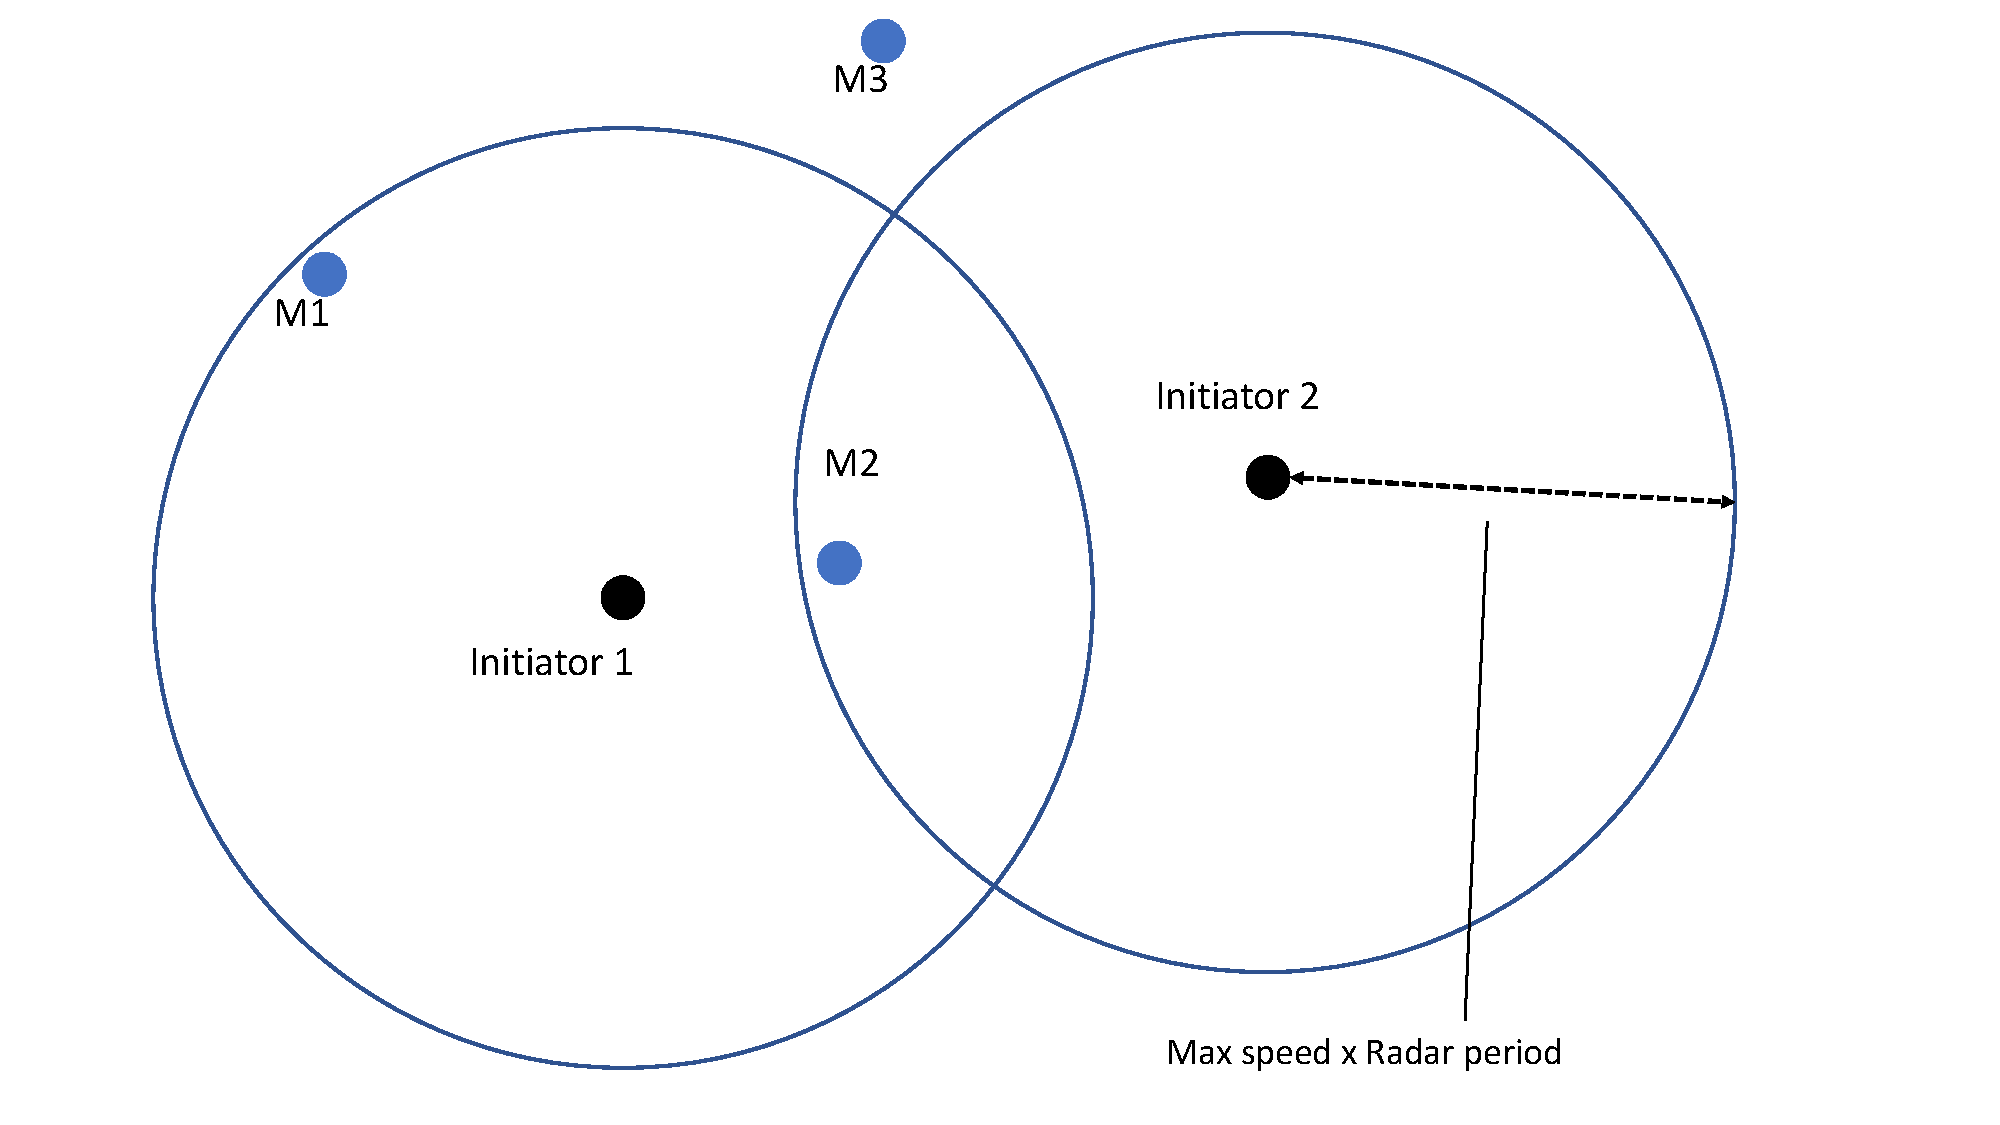
\includegraphics[width = .8\textwidth]{Figures/init_gating.pdf}
\caption{Initiator gating example}\label{fig:init_gating}
\end{figure}
If using method 1; to sequentially select the best, we have two possible outcomes. When starting with initiator 1, this initiator would be associated with measurement 2, and initiator 2 would not be associated with any measurements. On the other hand, starting with initiator 2 would lead to this initiator being associated with measurement 2, and initiator 1 would be associated with measurement 1. This randomness in outcome based on which initiator the algorithm starts with is clearly not a desired property. If using using method 2; to sequentially select the globally shortest distance, we would first associate initiator 1 with measurement 2, and there would not be any measurements left for initiator 2, leaving this empty.

A third option is to formulate the problem as a global combinatorial problem, and use an `off-the-shelf' solution to solve the problem. We have essentially a matrix with initiators along one axis and measurements along the second axis and the distance between them in their intersections, as in (\ref{eq:init_assignment_matrix}) for our example.
\begin{equation}\label{eq:init_assignment_matrix}
\kbordermatrix{
	 	& M_1 	& M_2 	& M_3	\\
    I_1 & 3 	& 1 	& 5 	\\
    I_2 & 7 	& 2 	& 6		\\
}
\end{equation}
The values above the threshold set by the maximum speed multiplied with the time period between the radar scans can be set to infinity to symbolise that this combination is not possible, see (\ref{eq:gated_init_assignment_matrix}) where the gate threshold is 4.
\begin{equation}\label{eq:gated_init_assignment_matrix}
\kbordermatrix{
	 	& M_1 		& M_2 	& M_3		\\
    I_1 & 3 		& 1 	& \infty 	\\
    I_2 & \infty 	& 2 	& \infty	\\
}
\end{equation}
If we remove the columns with only infinity, we are removing measurements that cannot be associated under any circumstances, thus reducing the size of the problem, see (\ref{eq:masked_gated_init_assignment_matrix}). With this pre processing, we want to assign each row to a column so that the sum of the selected intersections are minimal. 
\begin{equation}\label{eq:masked_gated_init_assignment_matrix}
\kbordermatrix{
	 	& M_1 		& M_2	\\
    I_1 & 3 		& 1  	\\ 
    I_2 & \infty 	& 2 	\\
}
\end{equation}
We now have formulated our problem in a way that it can be solved by the `Hungarian'\footnote{also known as the Munkres or Kuhn-Munkres algorithm} algorithm~\cite{Munkres1957}, which will give us the association \(I_1 \rightarrow M_1\) and \(I_2 \rightarrow M_2\). From the associations, a full state and new preliminary track is created with the latest measurement as position and velocity calculated based on the position difference divided by the time difference between the measurements. A preliminary track contains a state, initial covariance and counters of number of checks and passed checks. The initial covariance is a design variable and would be set according to the measurement and process noise.

\subsection{Process preliminary tracks}
When a new set of unused measurements arrive from the tracker, all the preliminary tracks are predicted to the time of the measurements. We now have the same association challenge between the predicted states and the measurements as with the initiators and measurements. Since we now have a full state and covariance for every preliminary track, we calculate the \gls{nis} for every combination of preliminary tracks and measurements, and selects the best combination. The preliminary tracks that are associated with a new measurement, their passed counter is incremented with one, while all preliminary tracks' checks counter is incremented with one. 

For preliminary tracks that have enough passed measurements, a new initial target is sent to the tracker. All preliminary tracks with check counter above the threshold is categorized as dead and deleted. 

\subsection{AIS aiding}
Since we might have AIS data available, it would be desirable to use this to improve the time and reliability of the initialization. In the same way as unused radar measurements are the input to the initialization procedure, we can use the unused AIS measurements to skip the first 2/2 filtering and create a preliminary track for each AIS measurement. This way we are giving the AIS measurements a little more `weight', but as this tracking system is based on AIS \emph{aiding} we still want the m/n filtering to be done with radar measurements. To avoid creating duplicate preliminary tracks for the same \gls{mmsi} over time, only unused AIS measurements with a MMSI not in the preliminary tracks are created. These choices are highly design specific and many other approaches is possible. 


\section{MHT Overview}
\begin{figure}
 \centering
 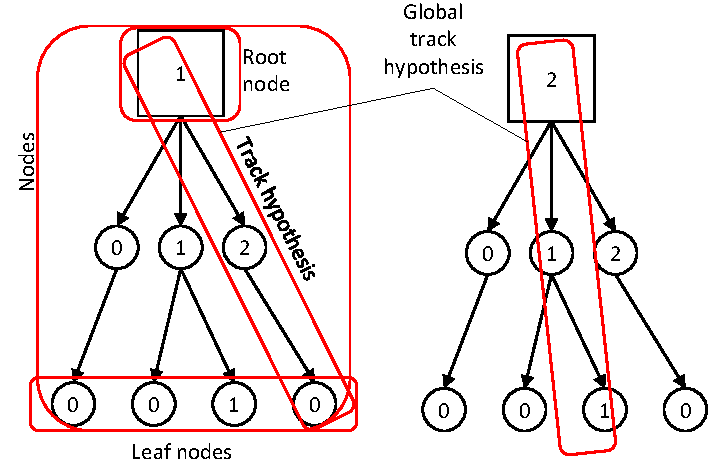
\includegraphics{Figures/Track-tree.pdf}
 \caption{Hypothesis tree}\label{fig:hyp_tree}
\end{figure}
The aim of this section is to outline the major steps in the MHT module and the flow of data and decisions. Figure~\ref{fig:algorithm_flow} shows the main steps that the module perform at each iteration / radar scan. The \gls{mht} algorithm is working on a set of \glspl{dag} or tree structures, often called a forest. The forest contains as many trees as targets the algorithm is tracking. Each tree consist of a root node and a set of child nodes, where each row represent a scan or discrete time. The leaf nodes are referred to as track hypotheses since leaf nodes represents itself and its parents.

 When new AIS and radar measurements are received, all leaf nodes are predicted forward to the time of the radar measurements. The radar measurements are then gated for each leaf node, and new pure radar hypotheses are generated for radar measurements within the gate. Each leaf node are then predicted to the time of the AIS measurements, and are gated at their time. AIS measurements inside the gate are then predicted to the time of the radar measurements where the radar measurements are gated based on each of the filtered AIS measurements. For each gated radar measurements give rise to fused hypotheses and from each AIS measurements without any radar measurement inside its gate a pure AIS hypothesis is created. Each new hypothesis is then given a score, which is the cumulative score of the parent node score and the new node's score. The target trees are then clustered according to which trees that shares measurements, whereon clusters with only one tree has the option of removing / merging similar hypotheses to reduce the size of the tree. For each cluster, the cluster-wise globally best association combination is selected using \gls{ilp}. Then, for each selected hypothesis the parent N steps above becomes the new root of that tree, and the unused children to the previous root node are removed. Next, targets whose best hypothesis have a score below the threshold is terminated, followed by the initialization of new targets from the initiator module. 

 The algorithm described in the three following sections are repeated for every leaf node in the forest. To avoid an extensive use of node- and measurement indexing the procedure is explained for one leaf node, with this node referred to as c---node, and is repeated for all leaf nodes in the forest. The c is only a symbol for indexing and referencing the chosen leaf node relative to predicted and filtered states. 
\begin{figure}[H]
\centering
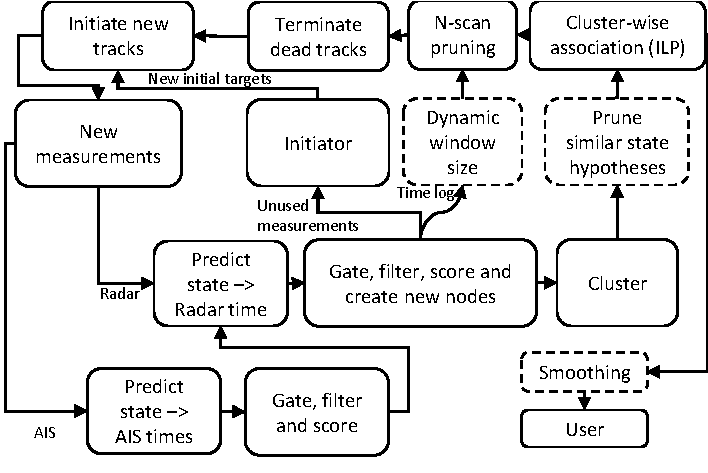
\includegraphics[width = \textwidth]{algorithm_flowchart.pdf}
\caption{Algorithm flowchart}\label{fig:algorithm_flow}
\end{figure}

To illustrate how this \gls{mht} system works we can look at an example of a target when it is turning. Figure~\ref{fig:hypotheses_when_turning} shows a single target which started in the lower left side doing a hard port turn followed by a straight course. The purple dots is the true track, the black dot is the stating position, the solid line is the selected/best hypothesis and the dotted lines are all the other hypotheses. As the target is turning, the zero hypotheses will continue in a straight line to allow for the possibility that there is a missed detection at that time. Most of the zero hypotheses are also splitting after their first and second scan upon creation, which can be seen as sharp angles between dotted lines moving outwards in the turn and dotted lines representing hypotheses which have re-connected with the true target.
\begin{figure}[H]
\centering
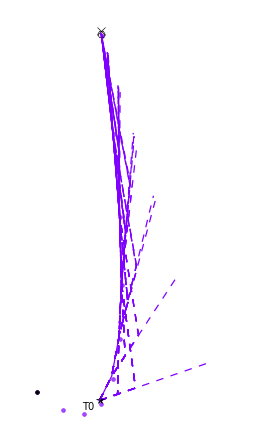
\includegraphics[height = .5\textheight]{Figures/Hypotheses_when_turning.PNG}
\caption{Hypotheses when turning}\label{fig:hypotheses_when_turning}
\end{figure}

\section{Process radar measurements}\label{sec:process_radar_measurements}
\subsection{Predict to radar time}
To compare new radar measurements with existing hypotheses, we should predict their states to the same time as the radar measurements, which can be done with the Kalman filter `time update' equation (\ref{eq:kalman_timeUpdate}) and the motion model from Section~\ref{sec:motion-model}. The residual covariance (\ref{eq:residual_covariance}), which is a part of the `measurement update' sequence of a Kalman filter are also calculated as the residual covariance is needed in the gating and these matrices are not dependent on the measurement residual.
\begin{equation}\label{eq:kalman_timeUpdate}
\begin{split}
\V{\bar{x}}_1 	&= \M{\Phi}(\Delta T_R) \V{x}_c \\
\M{\bar{P}}_1	&= \M{\Phi}(\Delta T_R) \M{P}_c \M{\Phi}^T(\Delta T_R) + \M{Q}(\Delta T_R) \\
\end{split}
\end{equation}
\begin{equation}\label{eq:residual_covariance}
\M{S}_1	= \M{H}\M{\bar{P}}_1 \M{H}^T + \M{R}_{Radar}
\end{equation}
\begin{equation*}
\begin{split}
\V{\bar{x}}		&= \text{predicted state} \\
\V{x}_c 		&= \text{origin node state} \\
\M{\bar{P}} 	&= \text{predicted state covariance} \\
\M{P}_c 		&= \text{origin node state covariance} \\
\Delta T_R 		&= \text{Radar time period} \\
\end{split}
\end{equation*}

\subsection{Gate}
To limit the number of hypotheses the leaf node have to create, the measurements are gated based on the leaf node's predicted covariance and a set confidence value. The size of the gate (Figure~\ref{fig:gating_radar_at_radar_time}) will reflect how insecure the prediction is, which is a function of how many detections and missed detections the leaf node and its parents have had. The gate (\ref{eq:gate}) is defined as \gls{nis} less than a threshold set by the inverse \(\chi^2\)--distribution \gls{cdf} with as many degrees of freedom as the measurement, two degrees of freedom for a maritime radar, and a set confidence value. A set of confidence levels and belonging \(\chi^2\) \gls{cdf} values are listed in Table~\ref{tab:chi_square}. The measurement residual and \gls{nis} is calculated for each measurement, and the measurements that does not pass the test are discarded.
\begin{figure}
\centering
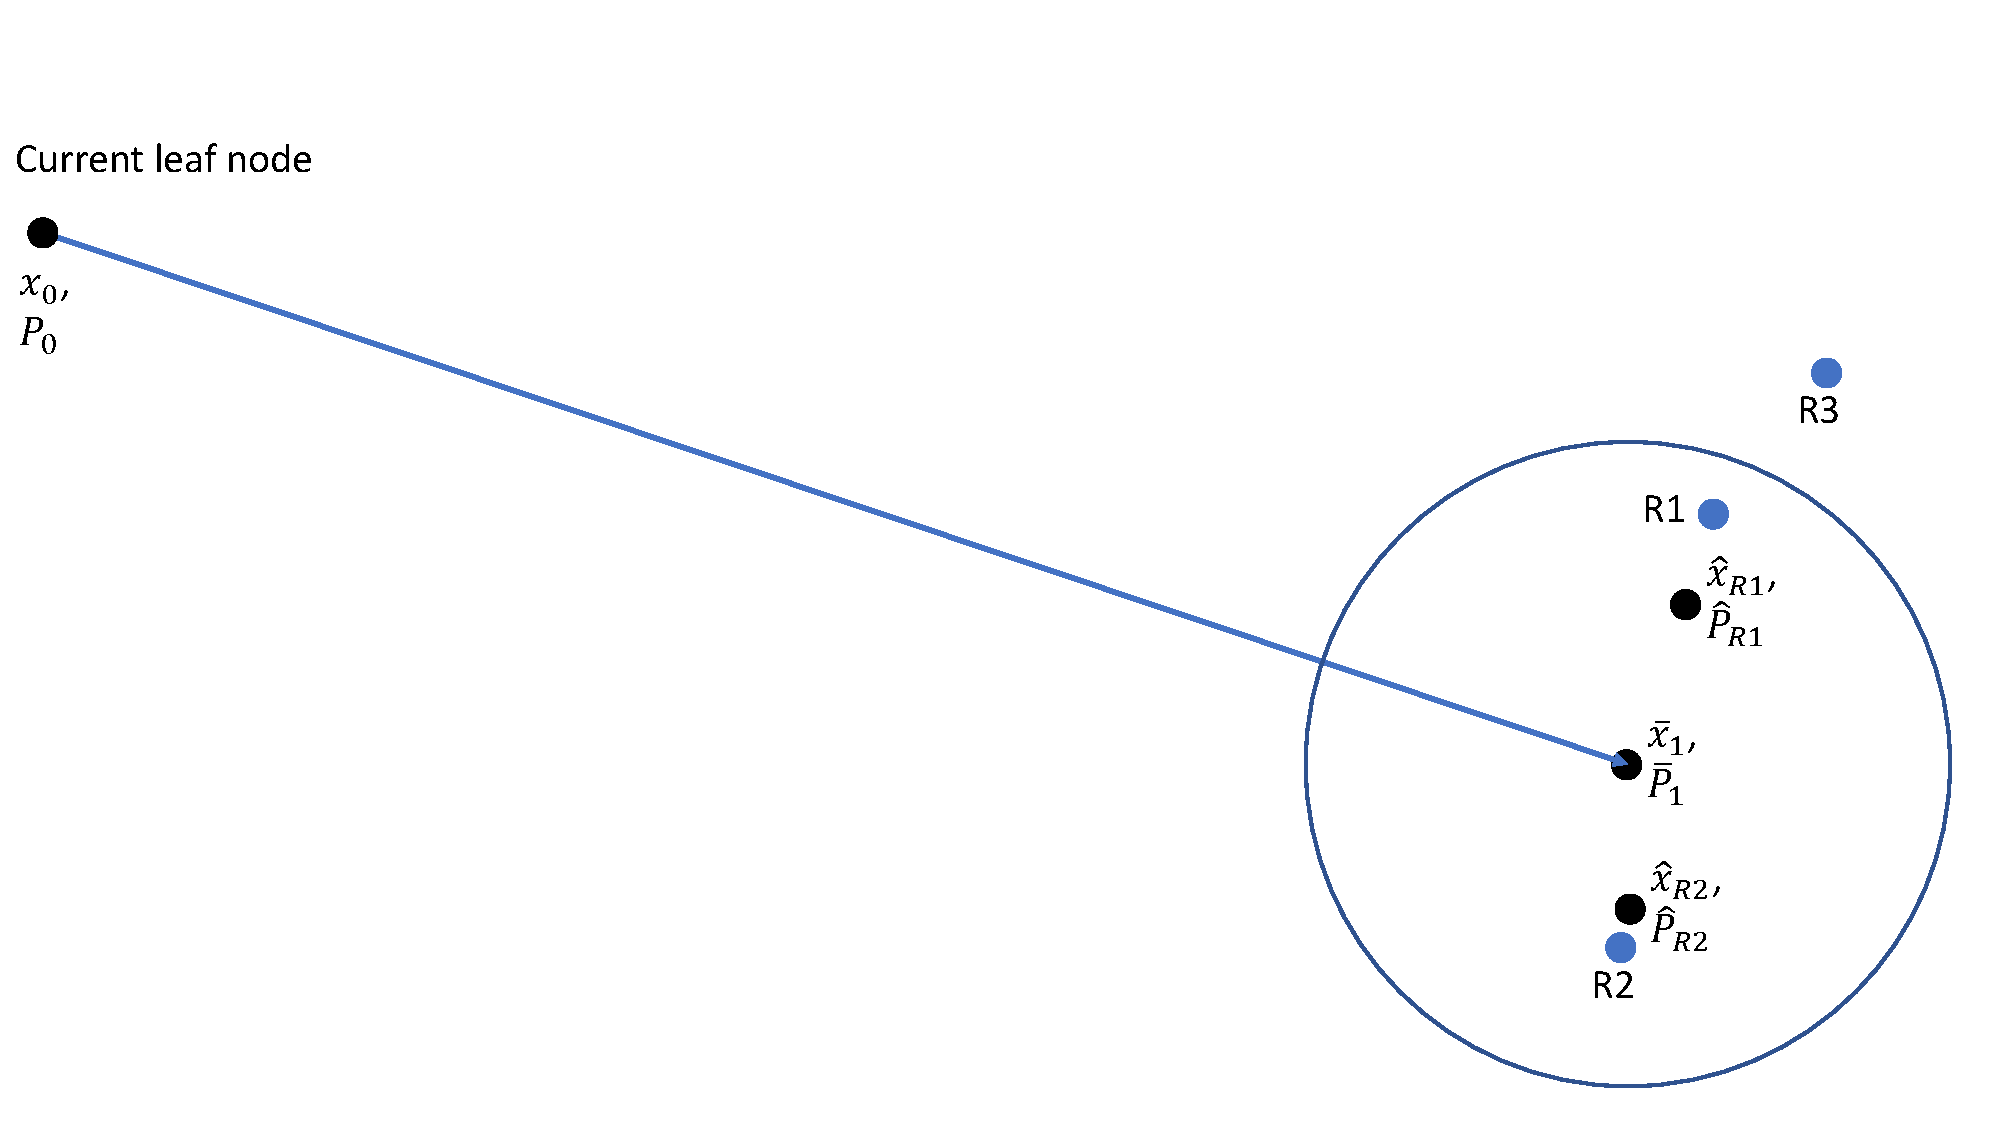
\includegraphics[width = .8\textwidth]{Figures/radar_gating.pdf}
\caption{Gating radar measurements at radar time}\label{fig:gating_radar_at_radar_time}
\end{figure}
\begin{equation}\label{eq:gate}
\begin{gathered}
\V{\tilde{z}} = \V{z} - \M{H}\V{\bar{x}}_1 \\
NIS = \V{\tilde{z}}^T	\M{S}^{-1} \V{\tilde{z}} \leq \eta^2
\end{gathered}
\end{equation}
\begin{equation*}
\begin{split}
\V{\tilde{z}}	&= \text{Measurement residual} \\
\eta^2 			&= \text{Gate size} \\
\end{split}
\end{equation*}
\begin{table}
\centering
\begin{tabular}{c c c c c c c c}
Confidence 	& 70\% 	& 80\% 	& 90\% 	& 95\% 	& 97.5\% 	& 99\% 	& 99.5\% \\ 
\midrule
\(\eta^2_{df=2}\) 	& 2.41 	& 3.22 	& 4.61 	& 5.99 	& 7.38 		& 9.21 	& 10.60
\end{tabular}\caption{Inverse \(\chi^2\) \gls{cdf} for two degrees of freedom}
~\label{tab:chi_square}
\end{table}

\subsection{Filter, score and create new nodes}
The scoring used in this tracking system is based on a dimensionless score function by Bar-Shalom~\cite{Bar-Shalom2007}. His paper discusses the issue of scoring measurement-to-track associations and comparing scores based on different numbers of measurement and measurement dimensions. He proposes a dimensionless \emph{likelihood ratio}, which is the \gls{pdf} of a measurement having originating from the track, divided by the \gls{pdf} of it not originating from the track. The outcome of not originating from the track is the union of the measurement being a clutter measurement and originating from a new target. The clutter and new target densities are both assumed Poisson distributed with \( \lambda_\nu \) being the new target density and \( \lambda_\phi \) the clutter density. The total extraneous measurement density is then \( \lambda_{ex} = \lambda_\nu + \lambda_\phi \). For numerical 

For each pure radar \gls{track hypothesis}, a \gls{nllr} (\ref{eq:radar_score_function}) is calculate, which is the negative natural logarithm of the score. The hypothesis is then scored with a \gls{cnllr}, which is the sum of its parent \gls{cnllr} and its own \gls{nllr}.
\begin{equation}\label{eq:radar_score_function}
\mathrm{NLLR}_{Radar} = \frac{1}{2} NIS + \ln \frac{\lambda_{ex} |2 \pi S|^{1/2}} {P_D}		
\end{equation}
\begin{equation}
\mathrm{CNLLR} \triangleq \sum NLLR
\end{equation}

\subsubsection{Zero hypothesis}\label{subsubsec:radar_zero_hypothesis}
To account for the possibility that the target is not present in this scan, a \emph{zero} hypothesis, or \emph{dummy} hypothesis as it is sometimes called, is generated with the predicted state and covariance \(\V{\bar{x}}_1, \M{\bar{P}}_1\). This node is numbered 0 in \Cref{fig:hyp_tree}, and \(\V{\bar{x}}_1\) in \Cref{fig:hyp_forest}.

\subsubsection{Pure radar hypotheses}
For every radar measurement (R1,R2 and R3 in \Cref{fig:gating_radar_at_radar_time}) inside the gate in (\ref{eq:gate}), a new track hypothesis (\(\V{\hat{x}}_{R1}\) and \(\V{\hat{x}}_{R2}\) in \Cref{fig:gating_radar_at_radar_time}) is generated with filtered state and covariance according to the regular Kalman `measurement update' equation (\ref{eq:kalman_measurement_update}).
\begin{equation}\label{eq:kalman_measurement_update}
\begin{split}
\M{K} 	&= \M{\bar{P}} \M{H}^T \M{S}^{-1} \\
\V{\hat{x}} &= \V{\bar{x}} + \M{K} \V{\tilde{z}} \\
\M{\hat{P}} &= \left(\M{I} - \M{K} \M{H} \right) \M{\bar{P}} \\
\end{split}
\end{equation}
\begin{equation*}
\begin{split}
\M{K}			&= \text{Kalman gain} \\
\M{S}			&= \text{Covariance innovation} \\
\M{\hat{P}}_1 	&= \text{filtered state covariance} \\
\end{split}
\end{equation*}

\section{Process AIS measurements}\label{sec:process_ais_measurements}
As elaborated in Section~\ref{sec:ais_preprocessing} all AIS measurements are preprocessed to remove out-of-order messages and ID-swap errors, and only the latest AIS update from each target (\gls{mmsi} number) are passed through to the MHT tracking loop. All \gls{ais} measurements outside the radar surveillance region are also removed from the measurement set.

The integration of AIS measurements into the MHT framework is not obvious and multiple approaches is possible. Since the AIS and radar measurement originate from different times, only sequential fusion methods~\cite{Bar-Shalom1995} are considered in this work. The first step in any approach would be to decide which AIS measurements the leaf node shall consider. The radar measurements usually arrive at fixed intervals and is normally not synchronized to an external clock. \gls{ais} on the other hand is transmitted at asynchronous intervals and the messages are time stamped with \gls{utc} time in whole seconds. These properties leads to a finite and in most cases relatively small number of possible \gls{ais} time stamps in between each radar scan. The long runtime for each iteration for a \gls{mht} algorithm favours synchronous processing of both \gls{ais} and \gls{radar} measurements at the arrival of each radar scan (synchronous processing). A choice that have to be made is if and when the \gls{ais} measurements should be gated. If no \gls{mmsi} are associated in a track hypothesis the most natural way might be to gate the \gls{ais} measurements in a somewhat similar fashion as the radar measurements. However, if a track hypothesis have been associated with an \gls{mmsi} previously, a natural approach could be to automatically associate this track hypothesis with new \gls{ais} measurement with the same \gls{mmsi}. This could most likely lead to a very good tracking as long as the \gls{mmsi} to target association is correct, but would lead to a divergence between the following radar measurements for the actual target and the falsely  associated \gls{ais} track. An alternative to the latest approach is to always gate the \gls{ais} measurements in some way and only allow track hypotheses which are already associated with an \gls{mmsi} to only accept \gls{ais} measurements with that \gls{mmsi}.

Since this MHT module is based on \gls{ais} aiding, the latest approach with continuous gating is chosen. This leads to two alternatives to gating; compare and gate AIS measurements at the AIS message times or predict the AIS measurements forward to the radar measurements time and gate at the same time as radar measurements.

\begin{algorithm}[H]
\caption{AIS gating at AIS time}\label{alg:ais_gating_at_ais_time}
\begin{algorithmic}[1]
\Procedure{Node::gateAisMeasurements}{AISmeasurements}
\State{} \(M0 \gets AISmeasurements\)
\State{}  aisTimes \( \gets \) Set(M0.times) 
\For{time \(\ in \) aisTimes}
\State{} \(T \gets time - node.time \)
\State{} \( \V{\bar{x}} = \M{\Phi}(T) \V{x_c} \)
\State{} \( \V{\bar{P}} = \M{\Phi}(T) \M{P_c} \M{\Phi}(T) + \M{Q}(T) \)
\State{} \( M1 \gets M0\) where measurement.time  == time
\State{} \( accuracySet \gets Set(M1.accuracy)\) \Comment{Accuracy can only be high or low}
\For{accuracy \(\ in \) accuracySet}
\State{} \(M2 \gets M1\) where measurement.accuracy == accuracy
\State{} \( \M{S} \gets \M{H}\M{\bar{P}}\M{H}^T + \M{R}_{accuracy} \)
\For{measurement \(in M2\)}
\State{} \( \V{z} \gets measurement.value \)
\State{} \( \V{\tilde{z}} \gets \V{z} - \M{H} \V{\bar{x}} \)
\State{} NIS \( \gets \V{\tilde{z}}^T \M{S}^{-1} \V{\tilde{z}} \)
\State{} aisInsideGate \( \gets NIS \leq \eta^2 \)
\If{aisInsideGate}
\State{} Filter \(\V{\bar{x}}\) with measurement
\State{} Predict to radar time
\For{radarMeasurement \(in\) radarMeasurements}
\State{} Gate radar measurement as with pure radar measurements
\For{radarMeasurement inside gate}
\State{} Create fused node
\EndFor{}
\EndFor{}
\EndIf{}
\EndFor{}
\EndFor{}
\EndFor{}
\EndProcedure{}
\end{algorithmic}
\end{algorithm}
Algorithm~\ref{alg:ais_gating_at_ais_time} outlines the main steps when gating at \gls{ais} times. The first step is to find all the different time stamps in the \gls{ais} \gls{measurement list}. Since most maritime radars operate between 24 and 48 \gls{rpm} and the AIS time in seconds is always integer, a maximum of 2 different AIS times will exist in between two radar scans of a 24 \gls{rpm} \gls{radar}. Then for each time in the time set, a predicted state and covariance is calculated and the measurements that are stamped with this time is picked out of the \gls{ais}measurement list. Since \gls{ais} messages transmit accuracy as either high or low, two different measurement covariances might be needed. The covariance residual is calculated for each accuracy among the \gls{ais} measurements, whereon the \gls{ais} measurements are gated, filtered and scored. The filtered state is then predicted to the radar time, where the predicted state and residual covariance are used to gate radar measurements as in Section~\ref{sec:process_radar_measurements}. In the situation were no radar measurements is inside the gate, a pure \gls{ais} hypothesis is created at the predicted state (radar time). Whether or not it is desirable to create an \gls{ais} `dummy' hypothesis / pure \gls{ais} hypothesis if there are any radar measurements inside the gate is a design choice. It will lead to a further increase in tree growth and computational cost, and might not lead to better tracking performance since the residual covariance after filtering with an \gls{ais} measurement would be relatively small and the difference between the pure \gls{ais} hypothesis and the fused hypotheses would be marginal.
\begin{figure}[H]
\centering
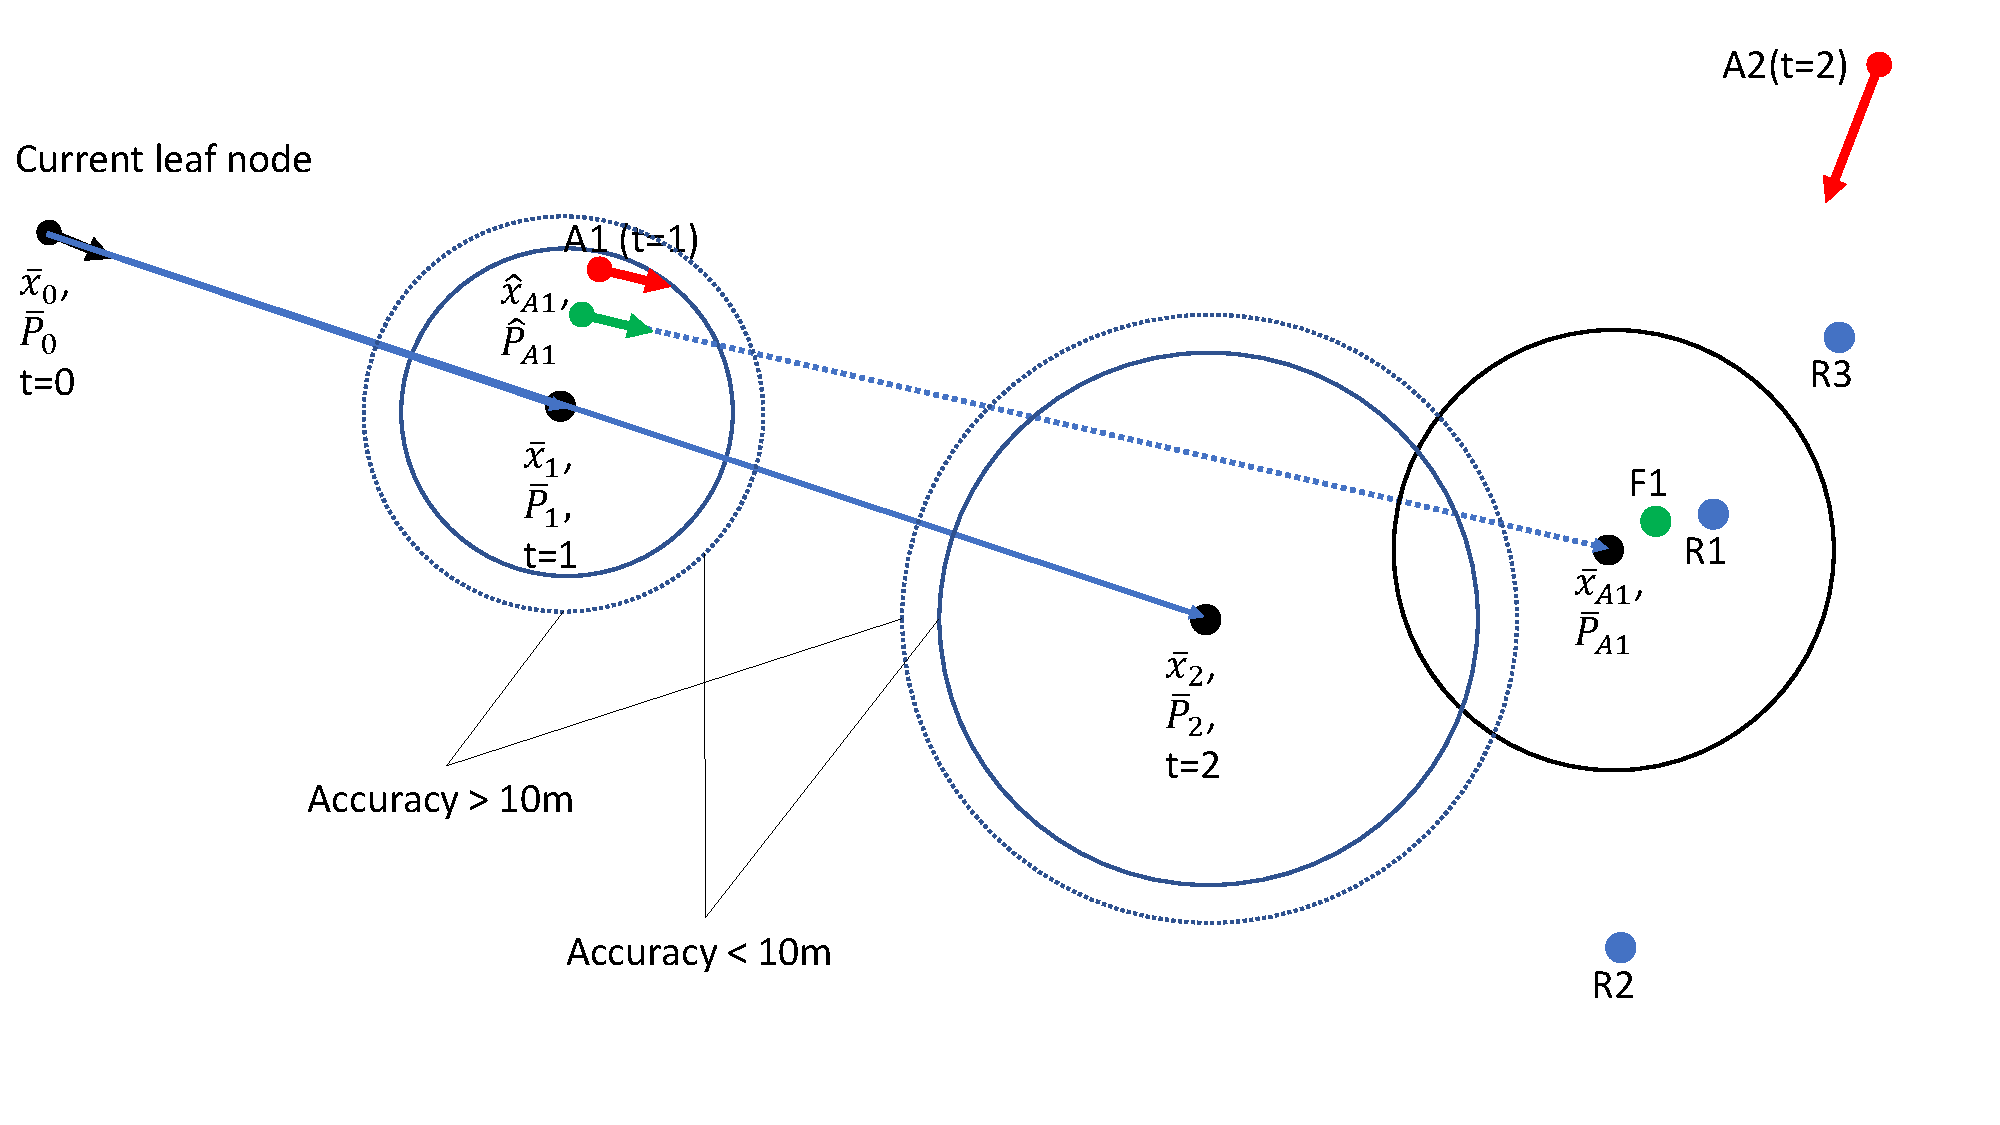
\includegraphics[width = .8\textwidth]{Figures/gating_at_ais_time.pdf}
\caption{Gating AIS at AIS time}\label{fig:gating_ais_at_ais_time}
\end{figure}
Figure~\ref{fig:gating_ais_at_ais_time} illustrates a situation where a single leaf node is showed in the upper left corner at \(t=0\), two red \gls{ais} measurements (A1 and A2) with position and velocity at \(t=1\) and \(t=2\) respectively and three blue radar measurements (R1, R2 and R3) at \(t=2.5\). \(\V{\bar{x}_1}\) and \(\V{\bar{x}_2}\) are the predicted states for \gls{ais} messages at \(t=1\) and \(t=2\) respectively, and the solid blue circles are representing the high accuracy gates while the dotted blue circles are representing the low accuracy gates. In this scenario only A1 is inside the \gls{ais} gates, and a filtered state \(\V{\hat{x}}_{A1}\) and covariance \(\M{\hat{P}}_{A1}\) is calculated. \(\V{\hat{x}}_{A1}\) is then predicted to \(t=2.5\) (\(\V{\bar{x}}_{A1}\) and \(\M{\bar{P}}_{A1}\)) and radar measurements are gated with the black solid circle based on the residual covariance to \(\M{\bar{P}}_{A1}\). Only R1 is inside this gate, thus a single fused hypothesis (F1) is created based on \(\V{\bar{x}}_{A1}\) filtered with R1.

\begin{figure}[H]
\centering
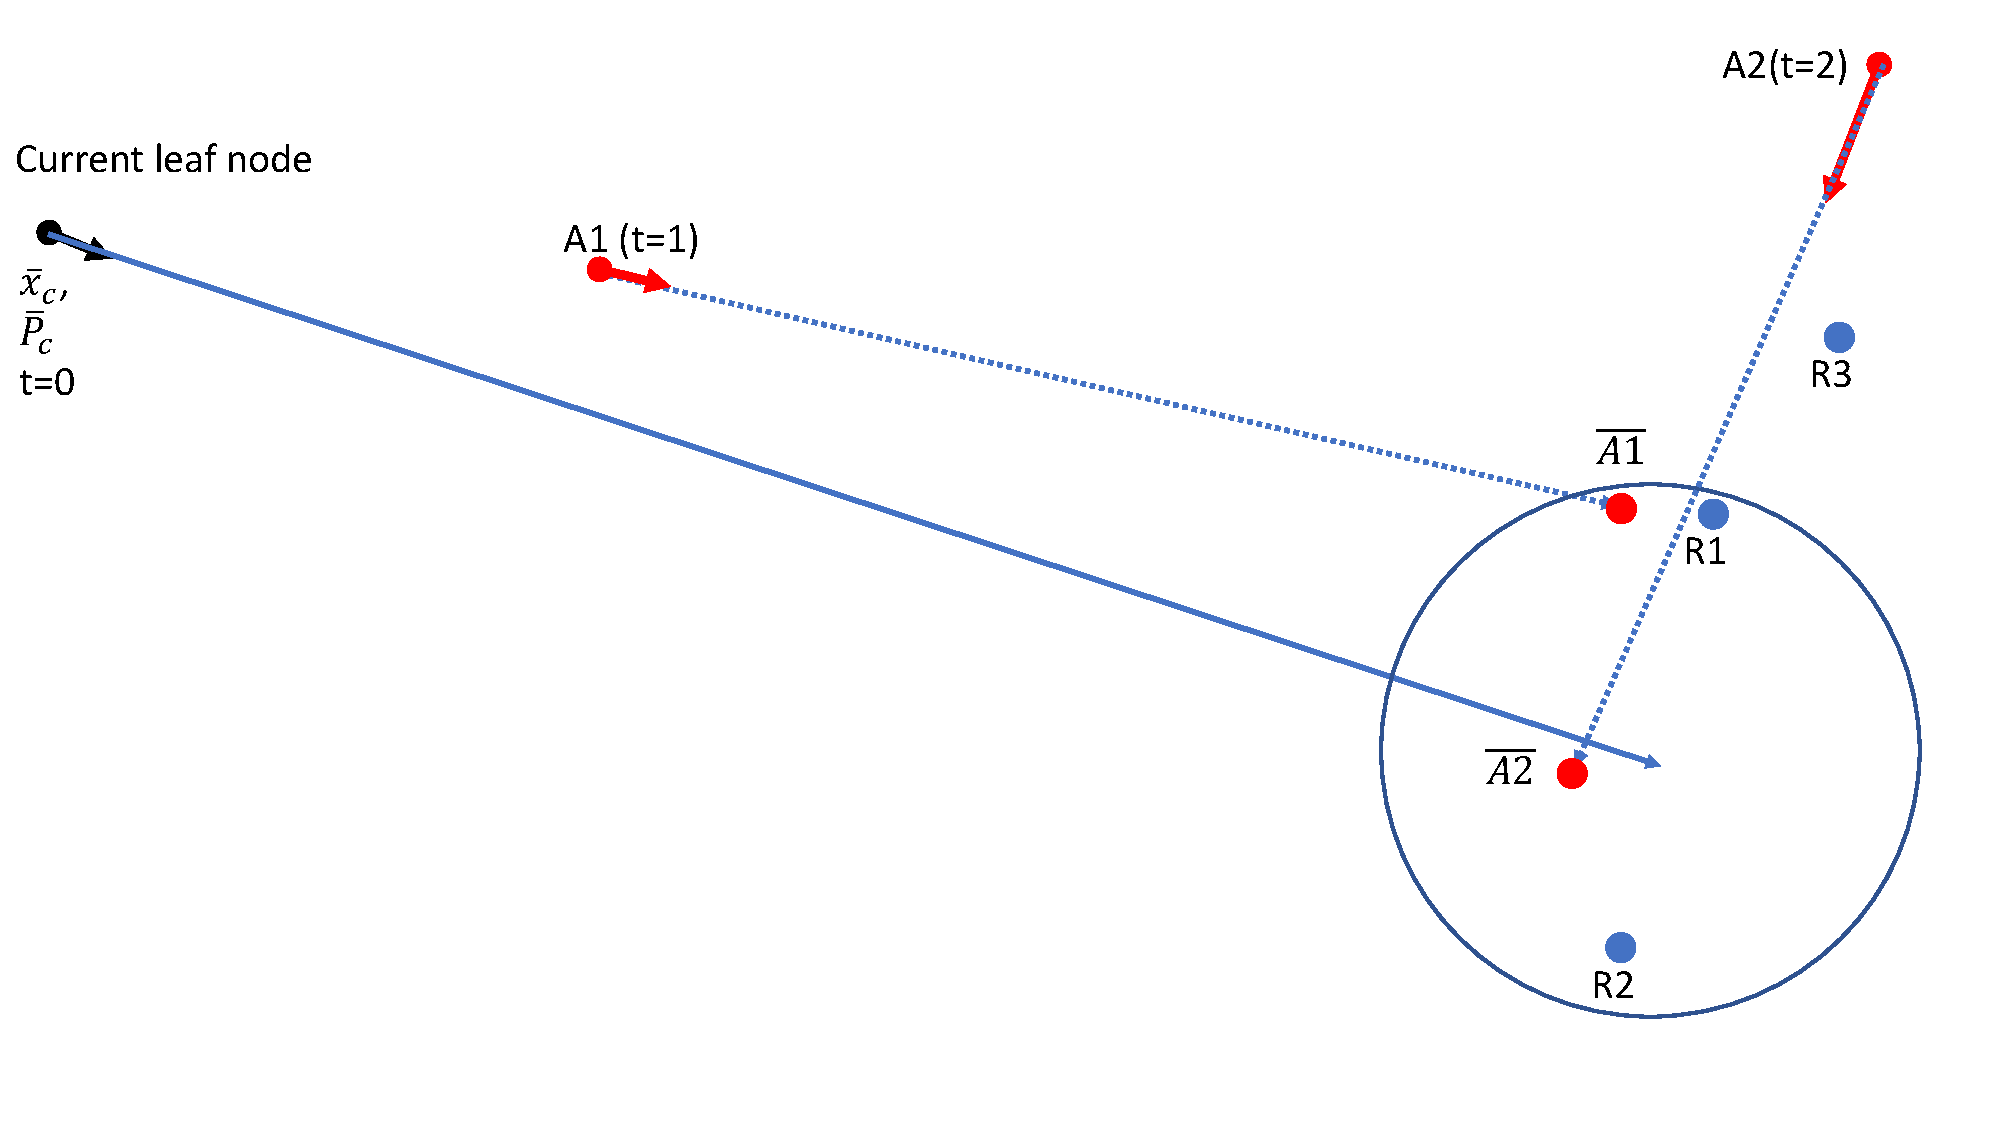
\includegraphics[width = .8\textwidth]{Figures/gating_at_radar_time.pdf}
\caption{Gating AIS at radar time}\label{fig:gating_ais_at_radar_time}
\end{figure}
If gating at radar time, all \gls{ais} measurements are predicted to radar time, and the predicted measurements are gated with the same gate at the radar measurements. By using the same gate on all measurements we assume that the radar measurement covariance is larger than the largest \gls{ais} measurement covariance, which is a reasonable assumption. This approach could however lead to unwanted AIS measurements inside the gate since the AIS measurements from other vessels can be predicted into the gate, thus leading to a more challenging association. This is exemplified in Figure~\ref{fig:gating_ais_at_radar_time}, where AIS measurement A2 would be inside the gate when gating at radar time but not if gating at \gls{ais} time. For all \gls{ais} measurements inside the gate, a complete set of fused hypotheses are created. In our example this would be (\(\overline{A1}\),R1), (\(\overline{A1}\), R2), (\(\overline{A2}\), R1) and (\(\overline{A2}\),R2). Since pure radar hypotheses are created prior to \gls{ais} processing it is not necessary to create any new pure radar hypotheses. 

In this work, the first approach is used for its assumed better performance and utilization of original data rather than predicted data. The \gls{ais} measurements are buffered between the radar scans, and pure \gls{ais} hypotheses are only created when no radar measurements fall inside the gate.

\subsection{Predict to AIS times}
To gate the AIS measurements, we first have to predict the target state and covariance (\ref{eq:predicted_origin_state_ais_time}) for each of the AIS time stamps (\ref{eq:ais_time_delta}) in the received AIS measurements. Since AIS only transmits a single integrity status, better or worse than 10 meter, maximum two possible \(\M{R}_{AIS}\) must be considered. With maximum two different time stamps and two different accuracies, a maximum of four different gates must be considered.
\begin{equation}\label{eq:ais_time_delta}
\begin{split}
\Delta T_{AIS_1} &= t_{AIS_1} - t_{c} \\
\Delta T_{AIS_2} &= t_{AIS_2} - t_{c} \\
\end{split}
\end{equation}

\begin{equation}\label{eq:predicted_origin_state_ais_time}
\begin{split}
\V{\bar{x}}_1 	&= \M{\Phi}(\Delta T_{AIS_1}) \V{x}_c \\
\M{\bar{P}}_1	&= \M{\Phi}(\Delta T_{AIS_1}) \M{P}_c \M{\Phi}^T(\Delta T_{AIS_1}) + \M{Q}(\Delta T_{AIS_1}) \\
\M{S}_{1_{High}}&= \M{H} \M{\bar{P}}_1 \M{H}^T + \M{R}_{AIS, High} \\
\M{S}_{1_{Low}}	&= \M{H} \M{\bar{P}}_1 \M{H}^T + \M{R}_{AIS, Low} \\
\V{\bar{x}}_2 	&= \M{\Phi}(\Delta T_{AIS_2}) \V{x}_c \\
\M{\bar{P}}_2	&= \M{\Phi}(\Delta T_{AIS_2}) \M{P}_c \M{\Phi}^T(\Delta T_{AIS_2}) + \M{Q}(\Delta T_{AIS_2}) \\
\M{S}_{2_{High}}&= \M{H} \M{\bar{P}}_2 \M{H}^T + \M{R}_{AIS, High} \\
\M{S}_{2_{Low}}	&= \M{H} \M{\bar{P}}_2 \M{H}^T + \M{R}_{AIS, Low} \\
\end{split}
\end{equation}

\subsection{Gate, filter and score}\label{sec:ais_gate_filter_score}
For each leaf node, all AIS measurements are gated with the gate matching their time, accuracy and threshold (Table~\ref{tab:chi_square_4_dof}). The measurements that pass the gating is then filtered with the predicted state and covariance matching its time, giving rise to an intermittent node (\ref{eq:filtered_ais_node}).
\begin{table}
\centering
\begin{tabular}{c c c c c c c c}
Confidence 	& 70\% 	& 80\% 	& 90\% 	& 95\% 	& 97.5\% 	& 99\% 	& 99.5\% \\ 
\midrule
\(\eta^2_{df=4}\) 	& 4.88 	& 5.99 	& 7.78 	& 9.49 	& 11.14 & 13.28	& 14.86
\end{tabular}\caption{Inverse \(\chi^2\) \gls{cdf} for four degrees of freedom}
~\label{tab:chi_square_4_dof}
\end{table}
\begin{equation}\label{eq:filtered_ais_node}
\V{\hat{x}}_1 = \V{\bar{x}}_1 + \M{K} \V{\tilde{z}}
\end{equation}

Depending on how we want the \gls{ais} to affect our tracking, two different scoring strategies are explored. The first approach is to view the \gls{ais} as a pure \emph{aiding}, where its only purpose is to improve the gating and uncertainty for the radar measurements. In this case, all \gls{ais} measurements are gated with a logarithmic score of zero, leading to neither improvement or worsening of the accumulative score of the track.

A second approach is to adapt the \gls{tomht} score function~\cite{Bar-Shalom2007} to the \gls{ais} paradigm. Since the \gls{ais} measurements are inherently labelled, then viewed from a single target, all \gls{ais} measurements except maximum one (depending on whether it have \gls{ais} transceiver or not) can be considered as clutter. If we then make the same assumptions as for radar measurements with respect to uniform spatial distribution and Poisson density distribution, we can estimate the expected number of \gls{ais} `clutter' measurements \( \lambda_{AIS} \) based on the amount of targets with \gls{ais} transmitters and the observation area (\ref{eq:ais_clutter_density}), where \(r_{radar}\) is the radar range. The clutter is in this context any measurement that does not belong to the target and which the target can erroneously utilize. The estimated clutter density could be calculated for a single frame, or averaged over a sliding window to reflect the \gls{ais} message flow over time since \gls{ais} transmission is not synchronised with the radar period. The resulting score function becomes (\ref{eq:ais_score_function2}).

\begin{equation}\label{eq:ais_clutter_density}
\lambda_{AIS} = \frac{n_{AIS}}{\pi r_{radar}^2}
\end{equation}

\begin{equation}\label{eq:ais_score_function2}
\mathrm{NLLR}_{AIS} = \frac{1}{2} NIS + \ln \lambda_{AIS} |2 \pi S|^{1/2} 
\end{equation}

Testing has shown that both the first and last method gives an improvement over pure radar tracking, and since the last method gives a little more improvement since it scores the \gls{ais} measurements with a reasonable values compared to the radar measurements, hence not giving the \gls{ais} measurements an enormous advantage or disadvantage. The second method is used in all the simulations in Chapter~\ref{chapter:results}.

\subsection{Predict to radar time}
All gated and filtered states from Section~\ref{sec:ais_gate_filter_score} is then predicted forward to the time of the radar measurements. This time delta will differ based on the time of the AIS measurement. Radar measurements are then gated for each predicted state and covariance, whereon a fused hypothesis are created for each radar measurement inside the gate. If there is no radar measurements inside the \gls{gate}, a pure \gls{ais} hypothesis are created. 

\subsubsection{Fused hypotheses}
The predicted state and covariance is then filtered with the gated radar measurement according to (\ref{eq:kalman_measurement_update}). The radar measurement is scored according to (\ref{eq:radar_score_function}), and the hypothesis score is a weighted sum of the AIS and radar score (\ref{eq:weighted_score}).
\begin{equation}\label{eq:weighted_score}
\mathrm{NLLR} = \frac{1}{2} \mathrm{NLLR}_{AIS} + \frac{1}{2} \mathrm{NLLR}_{Radar}
\end{equation}

\subsubsection{Pure AIS hypotheses}\label{subsec:pure_ais_hypotheses}
If no radar measurements are present in the gate, pure AIS hypotheses are created. This can be the situation when a target is broadcasting an AIS message, but is either in radar shadow or is not detected by the radar for any reason. These hypotheses are not created when one or more radar measurements are available, based on the assumption that if a radar measurement is present, the difference between a fused hypothesis and a pure AIS hypothesis is quite small since the AIS measurement covariance typically will be much smaller than the radar measurement covariance, leading to a fused state very close to the AIS measurement. The pure AIS hypothesis will use its predicted state and covariance and be  scored with \(\mathrm{NLLR}_{AIS}\), somewhat similar to radar zero hypotheses.

\section{Clustering}
The problem of finding the globally optimal set of track hypotheses increases exponentially with the number of hypotheses in the problem. To reduce the size of the problem, it is desirable to split it into smaller independent problems. Both because it enables parallel computation and it reduces the total cost of solving the problem. Track trees that have common measurements must be solved together, since they can have mutual exclusive leaf nodes. The clustering can be done efficiently through \gls{bfs} or \gls{dfs} on a graph made from the \gls{track hypothesis tree}.

By constructing a 0--1 adjacency matrix describing the connection between all the nodes in the \gls{track forest}, the clustering problem is equivalent to the \emph{connected components} problem in graph theory~\cite{Chen2015}.

\section{Optimal data association}\label{sec:optim_data_association}
The aim of this section is to elaborate the use of ILP to solve the data association problem in MHT that arises when there are multiple, possibly mutually exclusive, possibilities of measurement arrangements within the existing set of tracks. When the targets are divided into independent clusters, each of them can be treated as a global problem where we want to minimize the cost or maximize the score of the selected \glspl{track hypothesis} (leaf nodes). The selected \glspl{track hypothesis} must also fulfil the constraints, that each measurement can only be a part of one track, and that exactly one track hypothesis must be selected from each target. Since only binary values, selected or not selected, is possible for selection of hypotheses, the problem becomes an \gls{ilp}. In the case where a cluster is only containing one target tree, the best hypothesis can be selected by running a search among the leaf nodes after the highest score, since none of the leaf nodes are excluding other leaf nodes in other target trees. This will often be the case for targets that are largely spaced out, and their gates are not and have not overlapped in a while. For any other case, where there are two or more targets in a cluster, the procedure in Section~\ref{subsec:integer_linear_programming} must be carried out.

\subsection{Integer Linear Programming}\label{subsec:integer_linear_programming}
The essence of any optimization problem is a cost function and a set of constraints. In our problem, we want to select the combination of hypotheses (leaf nodes) that gives the highest score / lowest cost, while not selecting any measurement more than one time and ensure that we select minimum and maximum one hypothesis from each target. 

Our score function is the sum of the selected node scores, and since we are using negative logarithmic scores the goal is to minimize the overall score, making the problem a minimum cost problem. Our cost vector \(\V{c}\) is made up from the scores of all the leaf nodes in the forest build by the trees clustered together, arranged in the order they are visited by a \gls{dfs}. The accompanying selection vector \( \V{\tau} \) is of the same dimension with boolean values, where the selected hypotheses are value 1 and all other is value 0. These two together form the objective function (\ref{eq:objective_funtion}).
\begin{equation}
\begin{aligned}
& \underset{\V{\tau}}{\text{min}}
& & \V{c}^T \V{\tau}
\end{aligned}
\label{eq:objective_funtion}
\end{equation}

To ensure that we are selecting the same measurement maximum one time, a binary matrix \( \M{A_1} \) describing the association between nodes and measurements are created.\(\M{A_1}\) has as many rows are there are unique real measurement in the cluster forest and as as many columns as there are track hypotheses. All radar- and AIS measurement are real measurement, whereas dummy nodes do not contain any real measurements. Each rows in \( \M{A_1} \) represents a real measurements that exists in the cluster forest, and each column represents a track hypothesis. For each track hypothesis are the rows that represents the measurements used by that track hypothesis given value 1 (True) to indicate the usage. All other rows for that column are given value 0 (False) to indicate that it does not use these measurements. The order of the columns in \( \M{A_1} \) is the same as the rows in \( \V{c} \) and \( \V{\tau} \). Since we are only limiting a maximum of one usage of each measurement and no minimum, the constraint becomes an inequality constraint (\ref{eq:inequality_constraint}) where \( \V{1} \) is a vector of ones with the same dimension as \( \V{\tau} \).
\begin{equation}\label{eq:inequality_constraint}
\M{A_1} \V{\tau} \leq \V{1}
\end{equation}

The second constraint we need to impose is that we need to select exactly one track hypothesis from each tree. This can be done by creating a boolean matrix \( \M{A_2} \) which describes the relationship between hypotheses and trees / targets. \( \M{A_2} \) will have as many rows as there are targets in the cluster, and columns as \( \M{A_1} \). The intersections between hypotheses and targets that belong together is value 1, all other is value 0. Since this constraint has a fixed requirement, it is formulated as an equality constraint (\ref{eq:equality_constraint}) with \( \V{1} \) as in (\ref{eq:inequality_constraint}).
\begin{equation}\label{eq:equality_constraint}
\M{A_2} \V{\tau} = \V{1}
\end{equation}

The complete \gls{ilp} formulation becomes (\ref{eq:optim_formulation}), where \(\V{\tau}\) is a binary vector with dimension equal the number of leaf nodes in the track forest.
\begin{equation}
\begin{aligned}
&	\underset{\V{\tau}}{\text{max}}
&&	\V{c}^T \V{\tau} \\
&	\text{s.t.}
&&	\M{A_1} \V{\tau} \leq \V{b_1} 	\\
&&&	\M{A_2} \V{\tau} = \V{b_2}	\\
&&&	\V{\tau} \in {\{0,1\}}^{M}
\end{aligned}
\label{eq:optim_formulation}
\end{equation}

An example based on Figure~\ref{fig:hyp_forest} at time step 2, where the \(\M{A}\) matrices and \(\V{C}\) vector would be (\ref{eq:example_matrices}).
\begin{figure}[H]
\centering
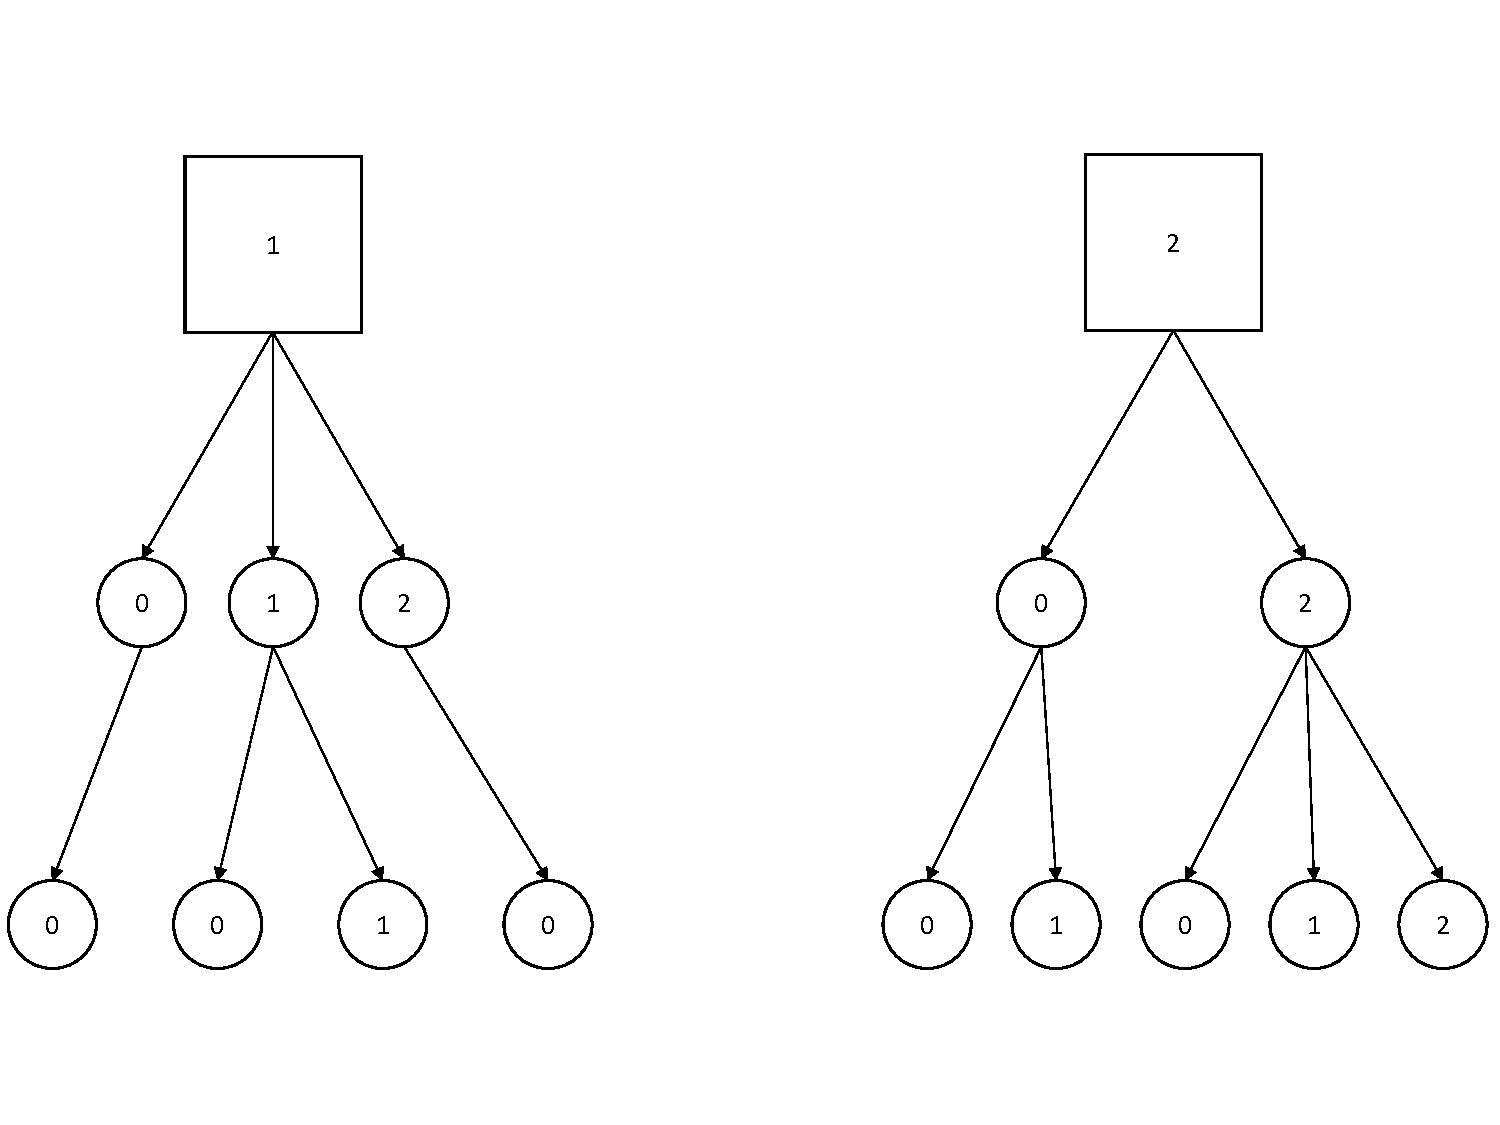
\includegraphics[clip, trim=0cm 2.5cm 0cm 2.5cm, width = .7\textwidth]{Track-forest}
\caption{Track hypotheses forest}\label{fig:hyp_forest}
\end{figure}

\begin{equation}
\begin{split}
\M{A_1} &=\begin{bmatrix}
		0 & 1 & 1 & 0 & 0 & 0 & 0 & 0 & 0 \\
       	0 & 0 & 1 & 0 & 0 & 1 & 0 & 1 & 0 \\
       	0 & 0 & 0 & 1 & 0 & 0 & 1 & 1 & 1 \\
       	0 & 0 & 0 & 0 & 0 & 0 & 0 & 0 & 1 \\
     	\end{bmatrix},\quad
\V{b_1} = 	\begin{bmatrix}
			1 \\ 1  \\ 1 \\ 1
			\end{bmatrix} \\
\M{A_2} &=\begin{bmatrix}
		1 & 1 & 1 & 1 & 0 & 0 & 0 & 0 & 0 \\
       	0 & 0 & 0 & 0 & 1 & 1 & 1 & 1 & 1 \\
     	\end{bmatrix} ,\quad
\V{b_2} = 	\begin{bmatrix}
			1 \\ 1
			\end{bmatrix} \\
\V{c} &=\begin{bmatrix}
		\lambda_1 & \lambda_2 & \lambda_3 & \lambda_4 & \lambda_5 & \lambda_6 & \lambda_7 & \lambda_8 & \lambda_9
		\end{bmatrix}^T \\
\end{split}
\label{eq:example_matrices}
\end{equation}

\subsection{Solvers}
The problem (\ref{eq:optim_formulation}) is formulated on standard form, which enables the use of existing off-the-shelf ILP solvers. There are a lot of off-the-shelf \gls{ilp} and \gls{milp} solvers on the marked, both free open source and commercial. The performance difference of some solvers were tested in~\cite{Liland_2017}, where the difference where found marginal,  most likely because each optimization problem is relatively small and the initialization and preprocessing of the solver and problem played a significant part of the runtime compared to the actual solving. In this work, Google Optimization Tools is used as interface between the programming language and the solver. The default solver CBC was used exclusively in this work as its performance was on par with the others tested in~\cite{Liland_2017}. 

\section{N-Scan pruning}
To keep the computational cost within reasonable limits, it is necessary to limit the amount of time steps backwards in time that the algorithm computes. This is done by removing all branches but the active track hypothesis at the current root node, and assign the one remaining node as new root node. This procedure is graphically explained in Figure~\ref{fig:pruned_tree}, where a solid square frame indicates the current root node, and a dotted square frame indicates the new root node. The bold arrows in the figure represents the active track.
\begin{figure}
\centering
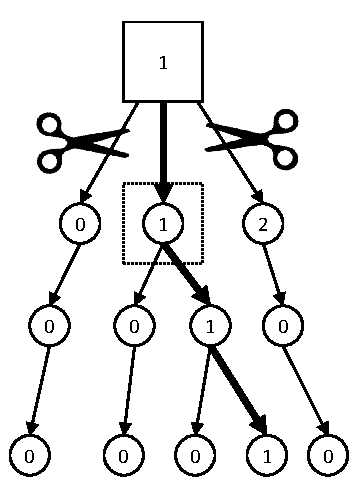
\includegraphics[scale = .8]{Figures/Pruned-tree.pdf}
\caption{N-scan pruning}\label{fig:pruned_tree}
\end{figure}

\subsection{Dynamic window}
For any MHT to be realistic over time it need to have a sliding window removing the unused hypotheses N steps back in time. The sliding window size (N) could be a static design parameter or a function of the runtime of that tree, which reflects the overall size of the tree. This enables the system to adapt its core parameters to guarantee its runtime demands. This scaling of N proved itself very efficient through testing and development, but is disabled in Chapter~\ref{chapter:results} for true comparison between different windows sizes.

\section{Track termination}
Since targets can disappear from the observation region both by leaving the radar range and by driving behind objects that puts them in a radar shadow, it is necessary to terminate these tracks. It is also desirable to terminate falsely initiated tracks as soon as possible, since a guidance system would steer clear of any objects reported to it. The first scenario, where the target is leaving the radar range can easily be detected and the track can be terminated quickly based on the predicted position of the target relative to our own position. The second scenario, can be approached in different ways depending on the available data and computational power. The simplest solution is to terminate all tracks where the selected node after each iteration have a score higher that a threshold. This could terminate tracks with consecutive miss detections, which is desirable for false tracks, but can lead to premature termination of true targets with temporarily low \gls{Pd}. This means that the termination threshold becomes a trade-of between killing false tracks and keeping targets with lower \gls{Pd} and shadowed targets. 

A more advanced approach could be to utilize map data to estimate whether or not a target is in a radar shadow of land objects, and then make a decision on whether this target should be given a lower \gls{Pd} temporary or terminated based. This could also be done between targets if target extent is estimated, where targets behind other targets are given a lower \gls{Pd} to punish miss detections less.

In this work, only range and score termination is implemented.

\section{Track smoothing}
After each iteration of the MHT algorithm a track list based on the selected hypotheses from Section~\ref{sec:optim_data_association} is passed forward to the operator and guidance system. Both human operators and guidance systems will try to predict the targets' behaviour based on their historical track. To improve the visualisation for this purpose it is possible to smooth the tracks based on the real measurements in the track and masking the dummy measurements in a Kalman smoother~\cite{Brown2012} with the same model as used in the predictions. As illustrated in Figure~\ref{fig:track_smoothing}, this will lead to a smother and in most cases a more accurate representation of the true track since it avoids the straight lines caused by dead reckoning. The circles represent dummy measurements, while it is real measurements on both sides of the dead reconing period (not plotted to avoid cluttered illustration). Figure~\ref{fig:track_smoothing_zoomed} is the same image zoomed in around the dead reconing area. This smoothing will however not affect the \gls{tracking} performance since it is done after miss detections are corrected and only on the track list sent out of the tracking module.
\begin{figure}[H]
\centering
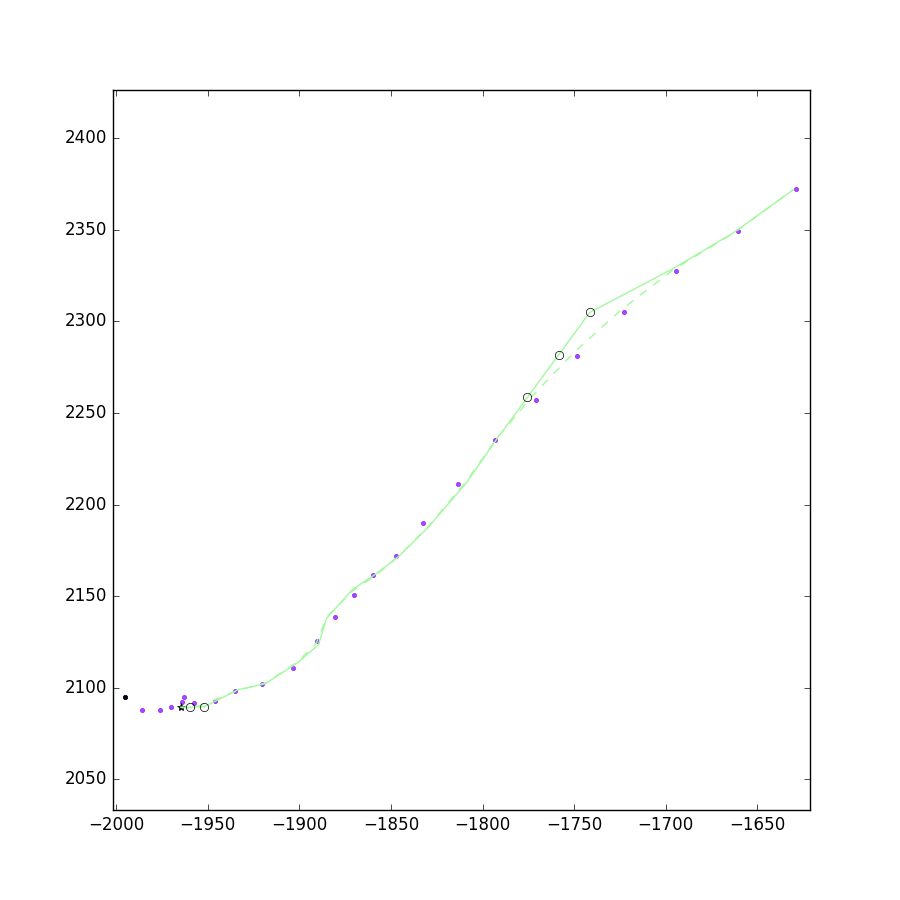
\includegraphics[trim={10cm 11cm 4cm 4cm},clip=true,height = .4\textheight]{Figures/track_smoothing_dummy_markers.png}
\caption{Track smoothing zoomed}\label{fig:track_smoothing_zoomed}
\end{figure}

\begin{figure}
\centering
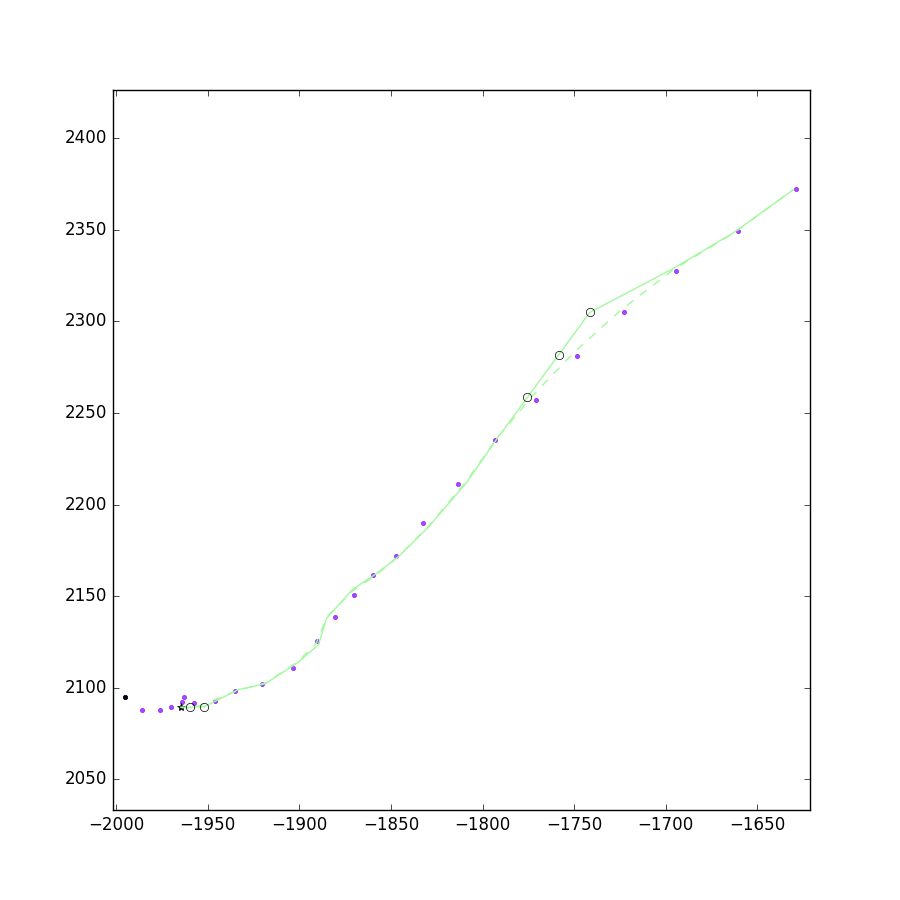
\includegraphics[width = .9\textwidth]{Figures/track_smoothing_dummy_markers.png}
\caption{Track smoothing}\label{fig:track_smoothing}
\end{figure}
 \clearpage 
	%!TEX root = ../TTK4900-MHT.tex

\chapter{Results}\label{chapter:results}
\section{Testing scheme}
The performance evaluation of the MHT tracking system is tedious in that it is necessary to test very many different situations to get a good understanding of how the system is performing. The two largest factors contributing to the difficulty is the random nature of the clutter and lost detections. It is also desirable to evaluate the initialization and tracking performance under both varying environmental (external) conditions and tuning (internal) setting. We want good tracking of targets with low probability of detections in cluttered environment, and secondly it must be able to do this within the time frame of the radar rotation period. The initialization module must be able to detect targets with probability of detection lower than unity without initializing too may false tracks into the MHT algorithm. The testing is separated into two parts; initialization and tracking.

The performance metrics for the initialization module is how long time it takes to initialize the correct tracks, which is tested under a range of internal and external conditions, see (\ref{eq:init_test_table}). All combinations of these parameters were simulated on all scenarios, see Table~\ref{tab:ais_scenarios}, which are the same routes but with different \gls{ais} configurations. From these simulations, the time to initiate true targets and amount of false targets are calculated. A track is categorized as correct initialized if the state difference between the true track and the initial track is less that a threshold. All initial tracks that does not correspond to a true track is categorized as erroneous. To analyse the impact of the erroneous tracks, the lifespan of falsely initiated tracks is plotted to see whether they die out at the same rate as they are initiated, or if they accumulate.  
\begin{equation}\label{eq:init_test_table}
\begin{split}
\V{P_D} &= \begin{bmatrix} 1.0 & 0.8 & 0.6 \end{bmatrix} \\
\V{M/N} &= \begin{bmatrix} 	(1/1) & (1/2) & (1/3) & (1/4) \\
							(2/2) & (2/3) & (2/4) & (2/5) \\
							(3/3) & (3/4) & (3/5) & (3/6)
		   \end{bmatrix} \\
\V{\lambda_\phi} &= \begin{bmatrix} 0 & 2\cdot10^{-6} & 4\cdot10^{-6} \end{bmatrix}
\end{split}
\end{equation}

When testing the tracking performance, it is desirable to remove the variable of initialization to better see difference in \emph{tacking} rather than \emph{initialization}. Therefore are all the simulations testing tracking performance carried out with all targets correctly initialized at initial time, and with the initiator set to \(M=2, N=4\) such that the unused measurements from the tracking algorithm would be treated as normal. This would also give lost targets a change to get re-initialized, which is an important property for any safety critical system.
\begin{equation}\label{eq:tracking_test_table}
\begin{split}
\V{P_D} &= \begin{bmatrix} 1.0 & 0.8 & 0.6 \end{bmatrix} \\
\V{N} &= \begin{bmatrix} 1 & 3 & 6 & 9 \end{bmatrix} \\
\V{\lambda_\phi} &= \begin{bmatrix} 0 & 2\cdot10^{-6} & 4\cdot10^{-6} \end{bmatrix}
\end{split}
\end{equation}
Since the targets are initialized perfectly in every situation, we are interested in how good our system is able to \emph{keep} on the tracks. We measure this by means of the Euclidean distance between the estimated and true track (\ref{eq:euclidian_distance_vector}).
\begin{equation}
	\Delta P = \| \V{p}_{track}-\V{p}_{target} \|_2
\label{eq:euclidian_distance_vector}
\end{equation}
The track is considered correct if \(\Delta P \leq \varepsilon_p\) for all t after initial convergence. If a track is deviating more than the threshold and never return within the threshold again, it is considered lost at the time-step when it exceeded the threshold. If the track should converge after exceeding the threshold, it is considered restored at the time-step it is returning within the limit. The second metric is how close the estimated track is to the true track on average. This is measured in \gls{rms} error of the entire track.

\section{Scenario}\label{sec:scenario}
All simulations in this work is based on a generated scenario, as shown in Figure~\ref{fig:test_scenario}, with black dots marking the initial time and position. The radar range is 5500 meter (~3 \glspl{nm_acr}), which gives an area of surveillance of approximately 95 square km. The scenario contains 16 targets, which all starts inside the observable area of the radar. The scenario contains a mixture of fast and slow moving vessels, some with sharp turns and some almost at stand still. Table~\ref{tab:init_states} shows the initial states of all targets, and the true path is generated once from these initial values.
\begin{figure}[H]
\centering
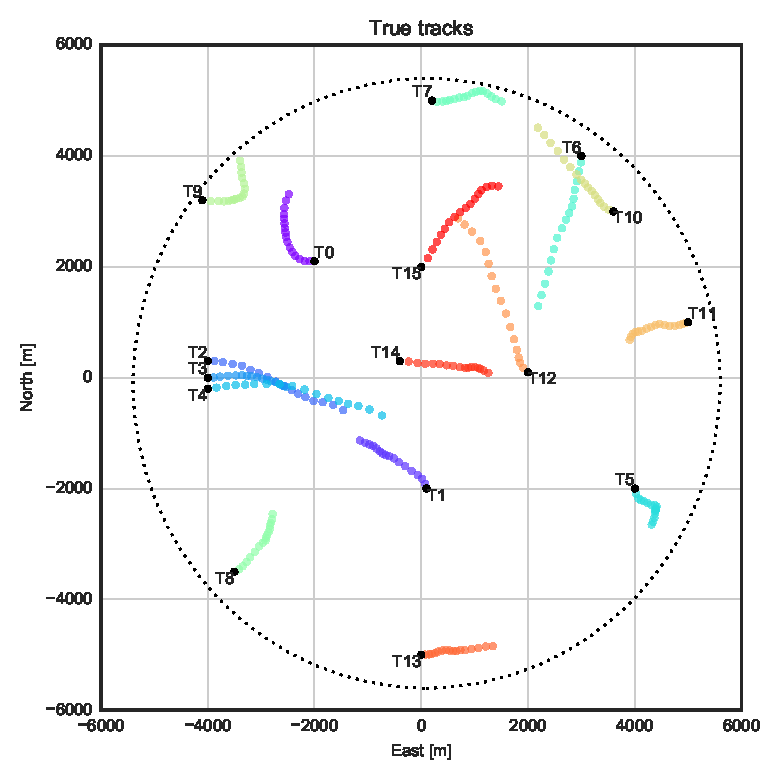
\includegraphics[width = .9\textwidth]{Figures/plots/ScenarioTruth.pdf}
\caption{True tracks}\label{fig:test_scenario}
\end{figure}

\begin{table}[H]
\centering
\begin{tabular}{c c c c c}
\bfseries Target & \bfseries North & \bfseries East & \bfseries North speed & \bfseries East speed \\ 
\toprule
\csvreader[head to column names,respect percent=true]{{Figures/plots/Scenario_Initial_State.csv}}{}
{\T{} & \NP{} & \EP{} & \NS{} & \ES{} \\}
\end{tabular}
\caption{Initial states}\label{tab:init_states}
\end{table}

From this base scenario, five scenarios where generated with different AIS configuration on the vessels, see Table~\ref{tab:ais_scenarios}. The first scenario represent the baseline with only radar information available, whereas the rest have some level of AIS information. Scenario 2 adds three class B AIS transmitters, and is representing a situation where all the targets are smaller vessels with some voluntarily installed AIS transceivers. In scenario 3, all vessels have AIS class B installed. This scenario represents a best case situation regarding yacht and leisure vessels from an autonomous anti collision perspective and is only realistic if AIS class B where to be mandatory for these vessel classes. Scenario 4 is the same as scenario 2, with the difference that the vessels have class A transmitters in stead of class B. This gives them higher and smarter rate of transmission, which in theory should improve tracking under challenging conditions. This scenario can be viewed as a few commercial vessels travelling in between a large group of yachts. The last scenario, where all targets are equipped with class A transmitters is the ultimate situation for any fusion tracking system. This case would be realistic in a crowded professional working area, for instance harbours, fishing areas and off-shore installations. 
\begin{table}
\centering
	\begin{tabularx}{0.5\textwidth}{XXXXXX}
	  \multicolumn{5}{c}{AIS scenario configuration} \\
	  \toprule
	  		 & \multicolumn{5}{c}{Scenario} \\
	  Target & 0 	& 1 	&  2 	&  3	& 4  	\\
	  \midrule
	  0 	& --- 	& --- 	& B 	& --- 	& A 	\\
	  1 	& --- 	& --- 	& B 	& --- 	& A 	\\
	  2 	& --- 	& --- 	& B 	& --- 	& A 	\\
	  3 	& ---	& B 	& B 	& A 	& A 	\\
	  4 	& --- 	& --- 	& B 	& --- 	& A 	\\
	  5 	& --- 	& --- 	& B 	& --- 	& A 	\\
	  6 	& --- 	& --- 	& B 	& --- 	& A 	\\
	  7 	& --- 	& --- 	& B 	& --- 	& A 	\\
	  8 	& --- 	& --- 	& B 	& --- 	& A 	\\
	  9 	& --- 	& --- 	& B 	& --- 	& A 	\\
	  10 	& --- 	& --- 	& B 	& --- 	& A 	\\
	  11	& ---	& B 	& B 	& A 	& A 	\\
	  12 	& --- 	& --- 	& B 	& --- 	& A 	\\
	  13 	& --- 	& --- 	& B 	& --- 	& A 	\\
	  14 	& ---	& B 	& B 	& A 	& A 	\\
	  15 	& --- 	& --- 	& B 	& --- 	& A 	\\
	  \bottomrule
	\end{tabularx}~\caption{AIS scenario configuration}\label{tab:ais_scenarios}
\end{table}

\section{Simulation}
Both initialization- and tracking performance is averaged over a set of 50 Monte Carlo simulations with differently seeded clutter- and detections points. All simulations are done with a sampling interval at 2.5 seconds (24 \gls{rpm}), which is the most common rotation speed on a coastal maritime radar. Each of the 108 initialization variations and 180 track performance simulations where run 50 times with different seeded clutter and misdetections on a dual Intel i7--6700 processor and \gls{ssd} storage. 
 \clearpage %##Contains ArialMT type 3 linked fonts##
	%!TEX root = ../TTK4900-MHT.tex

\chapter{Discussion}\label{chapter:discussion}
Discussion here.

\section{Alternative design / open questions}
What to do when a track previously associated with an MMSI no longer has new AIS measurements from that MMSI inside its gate? Make an extra hypothesis with a jump? An how to score this?

What to do with unused AIS measurements, i.e. ones that are not previously associated with any tracks and are not within any gate? Use them as measurements in the initialization procedure? Initiate them as new tracks immediately?

In what ways can AIS meta-data improve the radar tracking? From AIS length information, it might be possible to estimate the maximum turning rate for a vessel.
 \clearpage  
	%!TEX root = ../TTK4900-MHT.tex

\chapter{Future work}\label{chapter:future-work}
Optimalization based pruning

Multi core implementation

 \clearpage  
	%!TEX root = ../TTK4900-MHT.tex

\chapter{Conclusion}\label{chapter:conclusion}
To the knowledge of the author, this thesis has presented the first \gls{mht} implementation utilizing both \gls{ais} and \gls{radar} information. It has shown the benefits of using \gls{ais} to aid an \gls{ilp} based track oriented \gls{mht} integrated into a complete tracking system. The behaviour and performance for different tuning parameter in a logic based track initiator has also been demonstrated.
Through simulations it has been shown that targets with low probability of detection benefits greatly from \gls{ais} aiding, whereas targets with moderate to high probability of detection gained less benefits.  \clearpage  
	\makeatletter\@openrightfalse\makeatother 
	%!TEX root = ../TTK4900-MHT.tex

\begin{appendices}
	%!TEX root = ../TTK4900-MHT.tex

\chapter{Initialization time plot}

\begin{figure}[H]
\centering
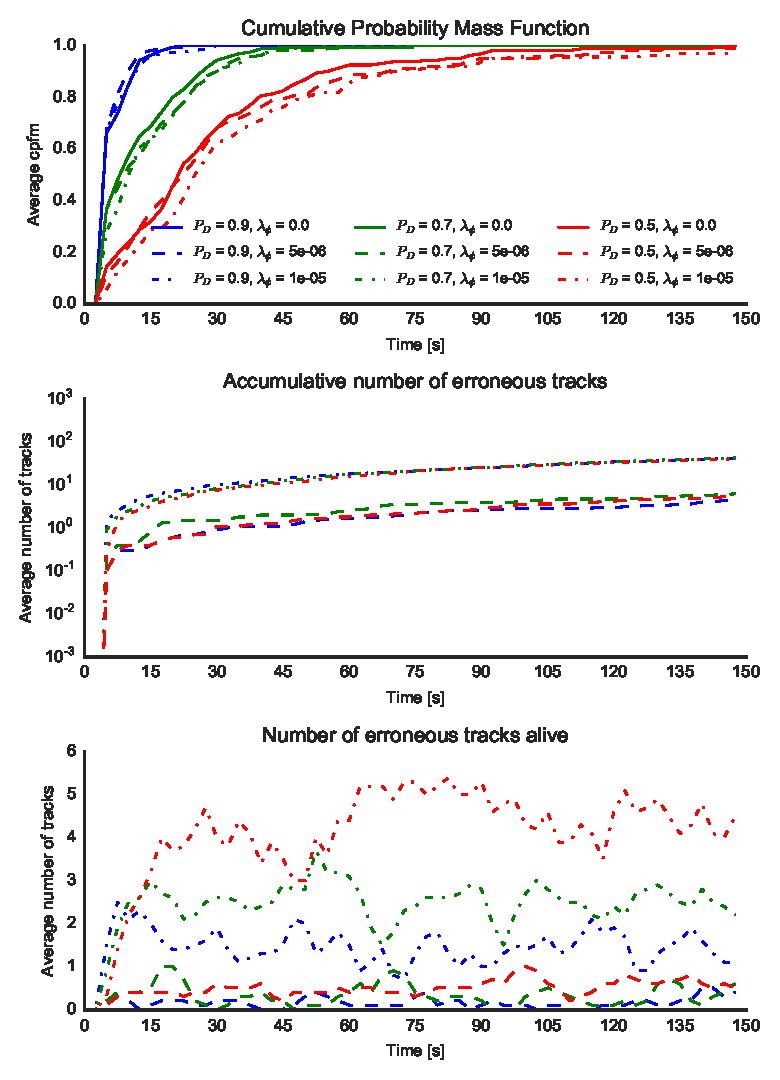
\includegraphics[height = .9\textheight]{Figures/plots/Scenario1_Init-Time(1-1).pdf}
\caption{Initialization time (1/1)}\label{fig:init_time_1-1}
\end{figure}

\begin{figure}
\centering
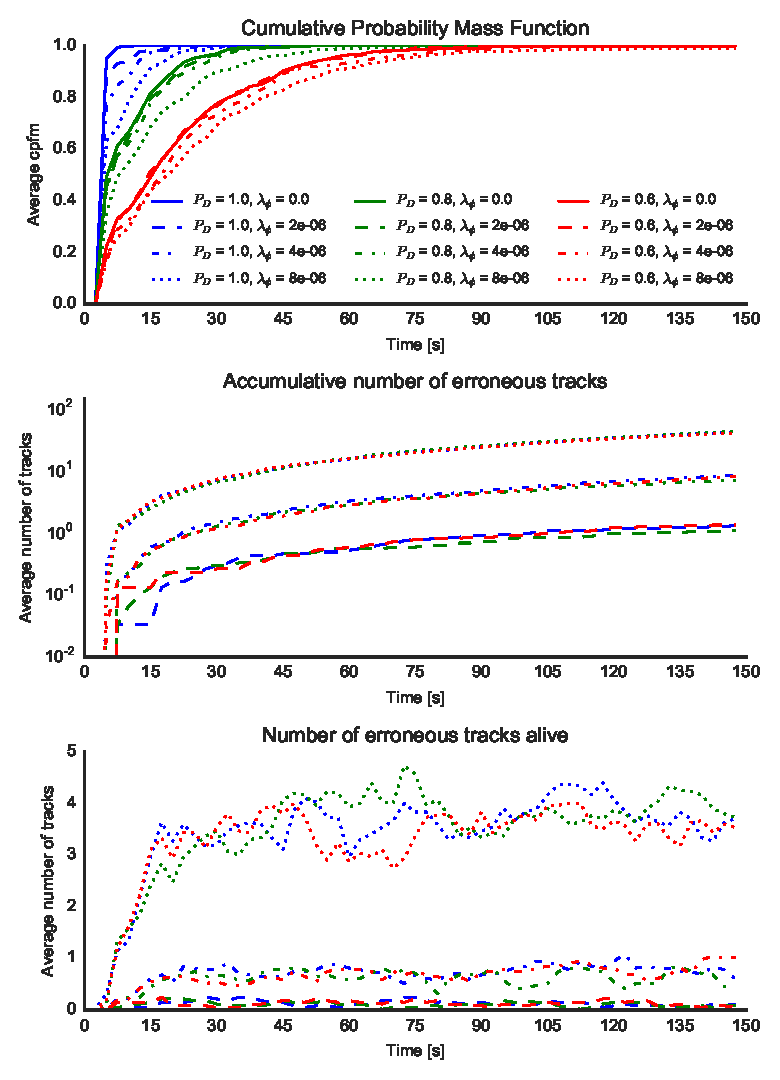
\includegraphics[height = .9\textheight]{Figures/plots/Scenario1_Init-Time(1-2).pdf}
\caption{Initialization time (1/2)}\label{fig:init_time_1-2}
\end{figure}

\begin{figure}
\centering
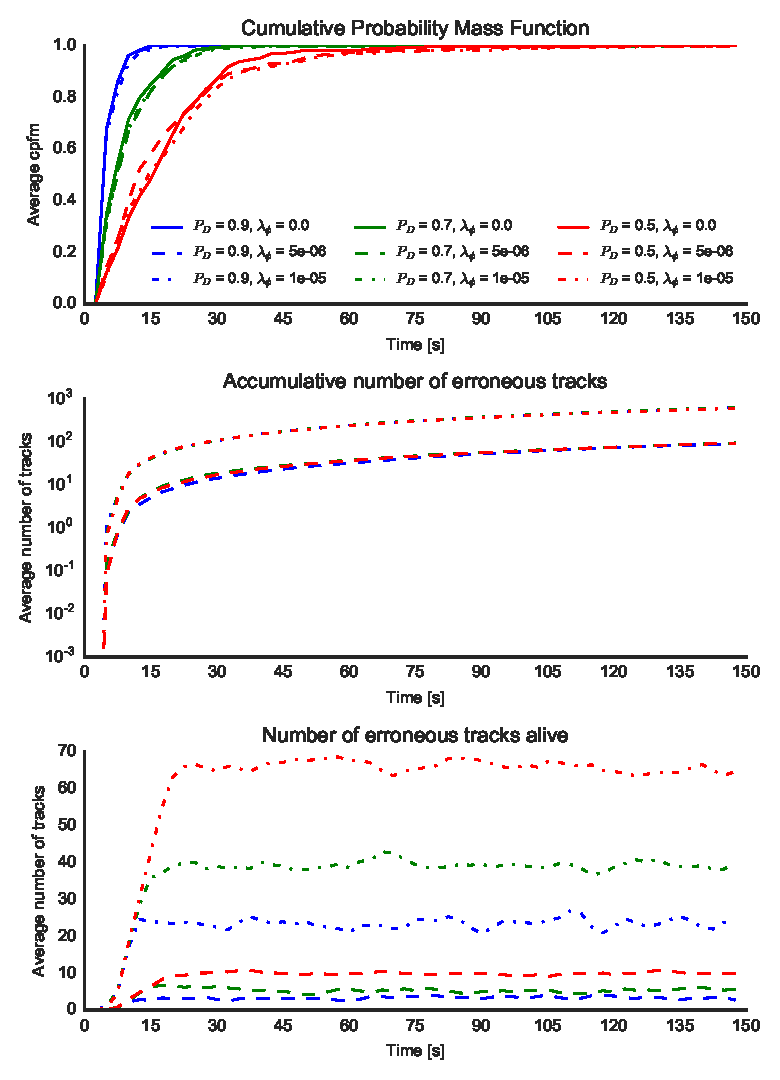
\includegraphics[height = .9\textheight]{Figures/plots/Scenario1_Init-Time(1-3).pdf}
\caption{Initialization time (1/3)}\label{fig:init_time_1-3}
\end{figure}

\begin{figure}
\centering
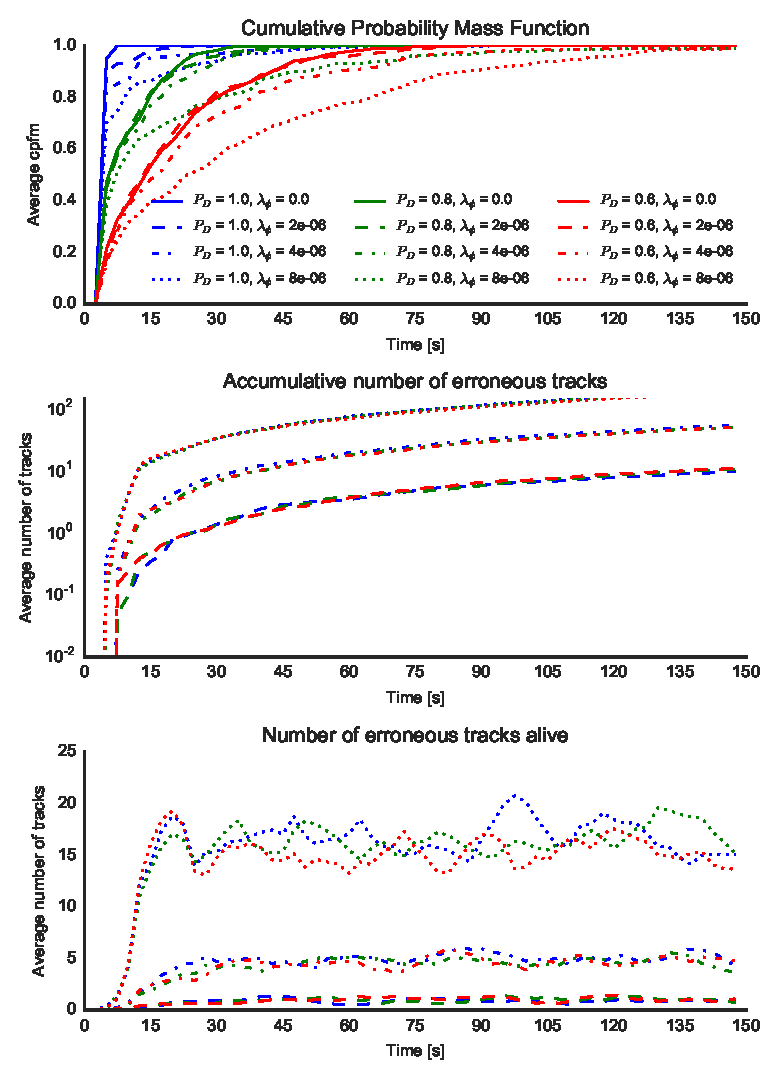
\includegraphics[height = .9\textheight]{Figures/plots/Scenario1_Init-Time(1-4).pdf}
\caption{Initialization time (1/4)}\label{fig:init_time_1-4}
\end{figure}

\begin{figure}
\centering
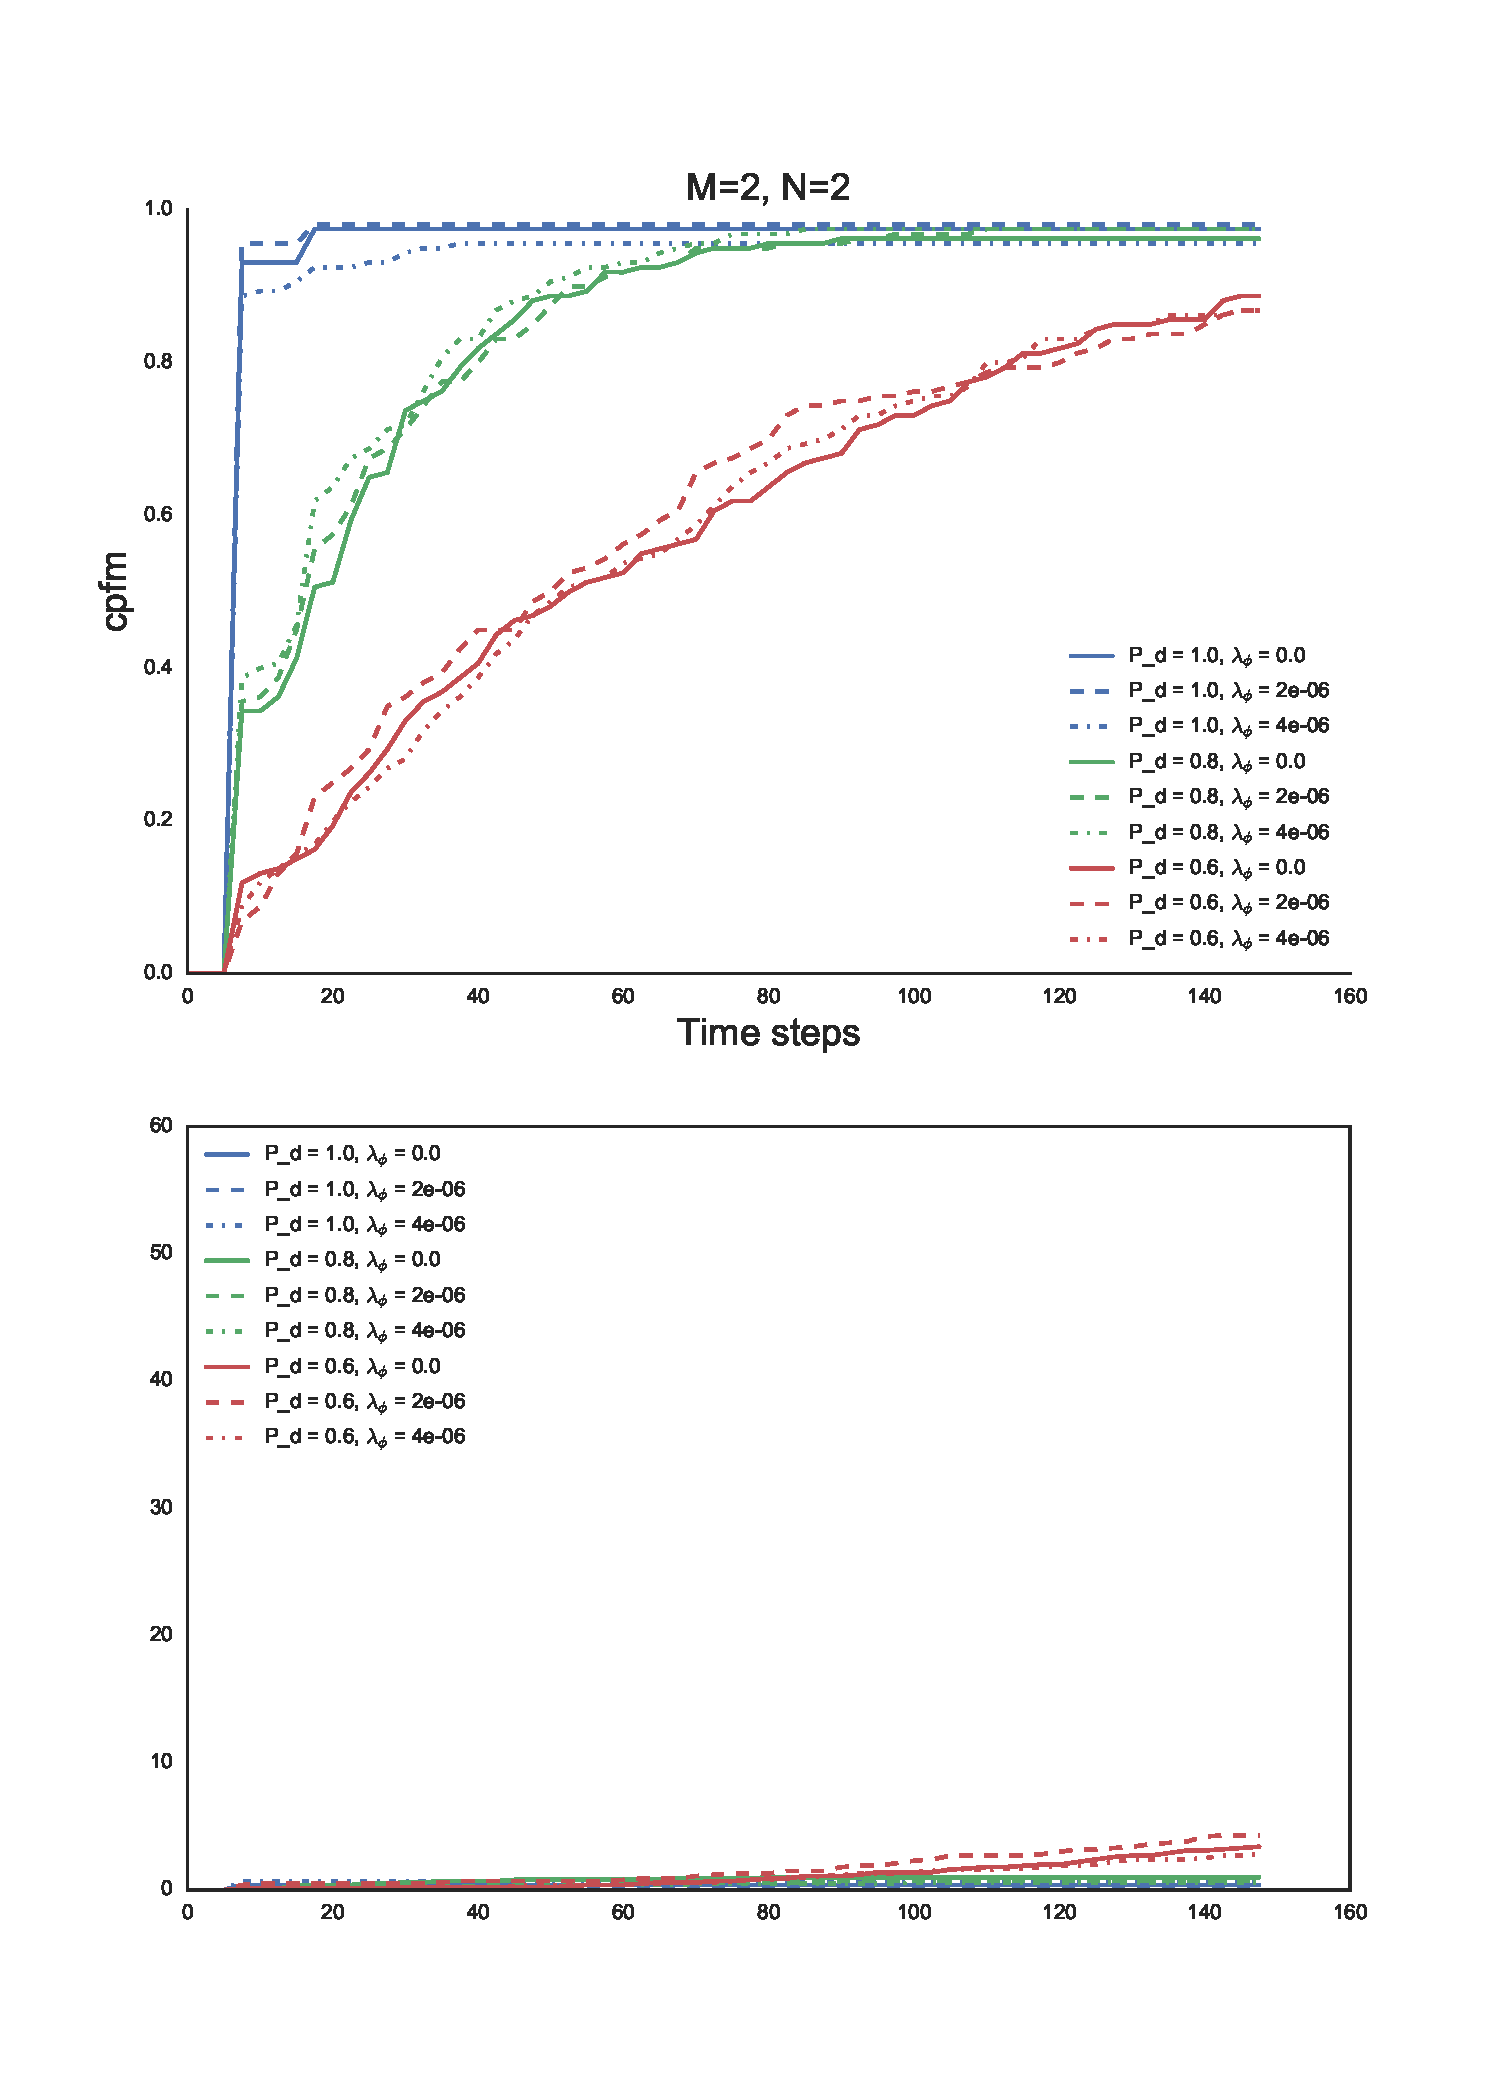
\includegraphics[height = .9\textheight]{Figures/plots/Scenario1_Init-Time(2-2).pdf}
\caption{Initialization time (2/2)}\label{fig:init_time_2-2}
\end{figure}

\begin{figure}
\centering
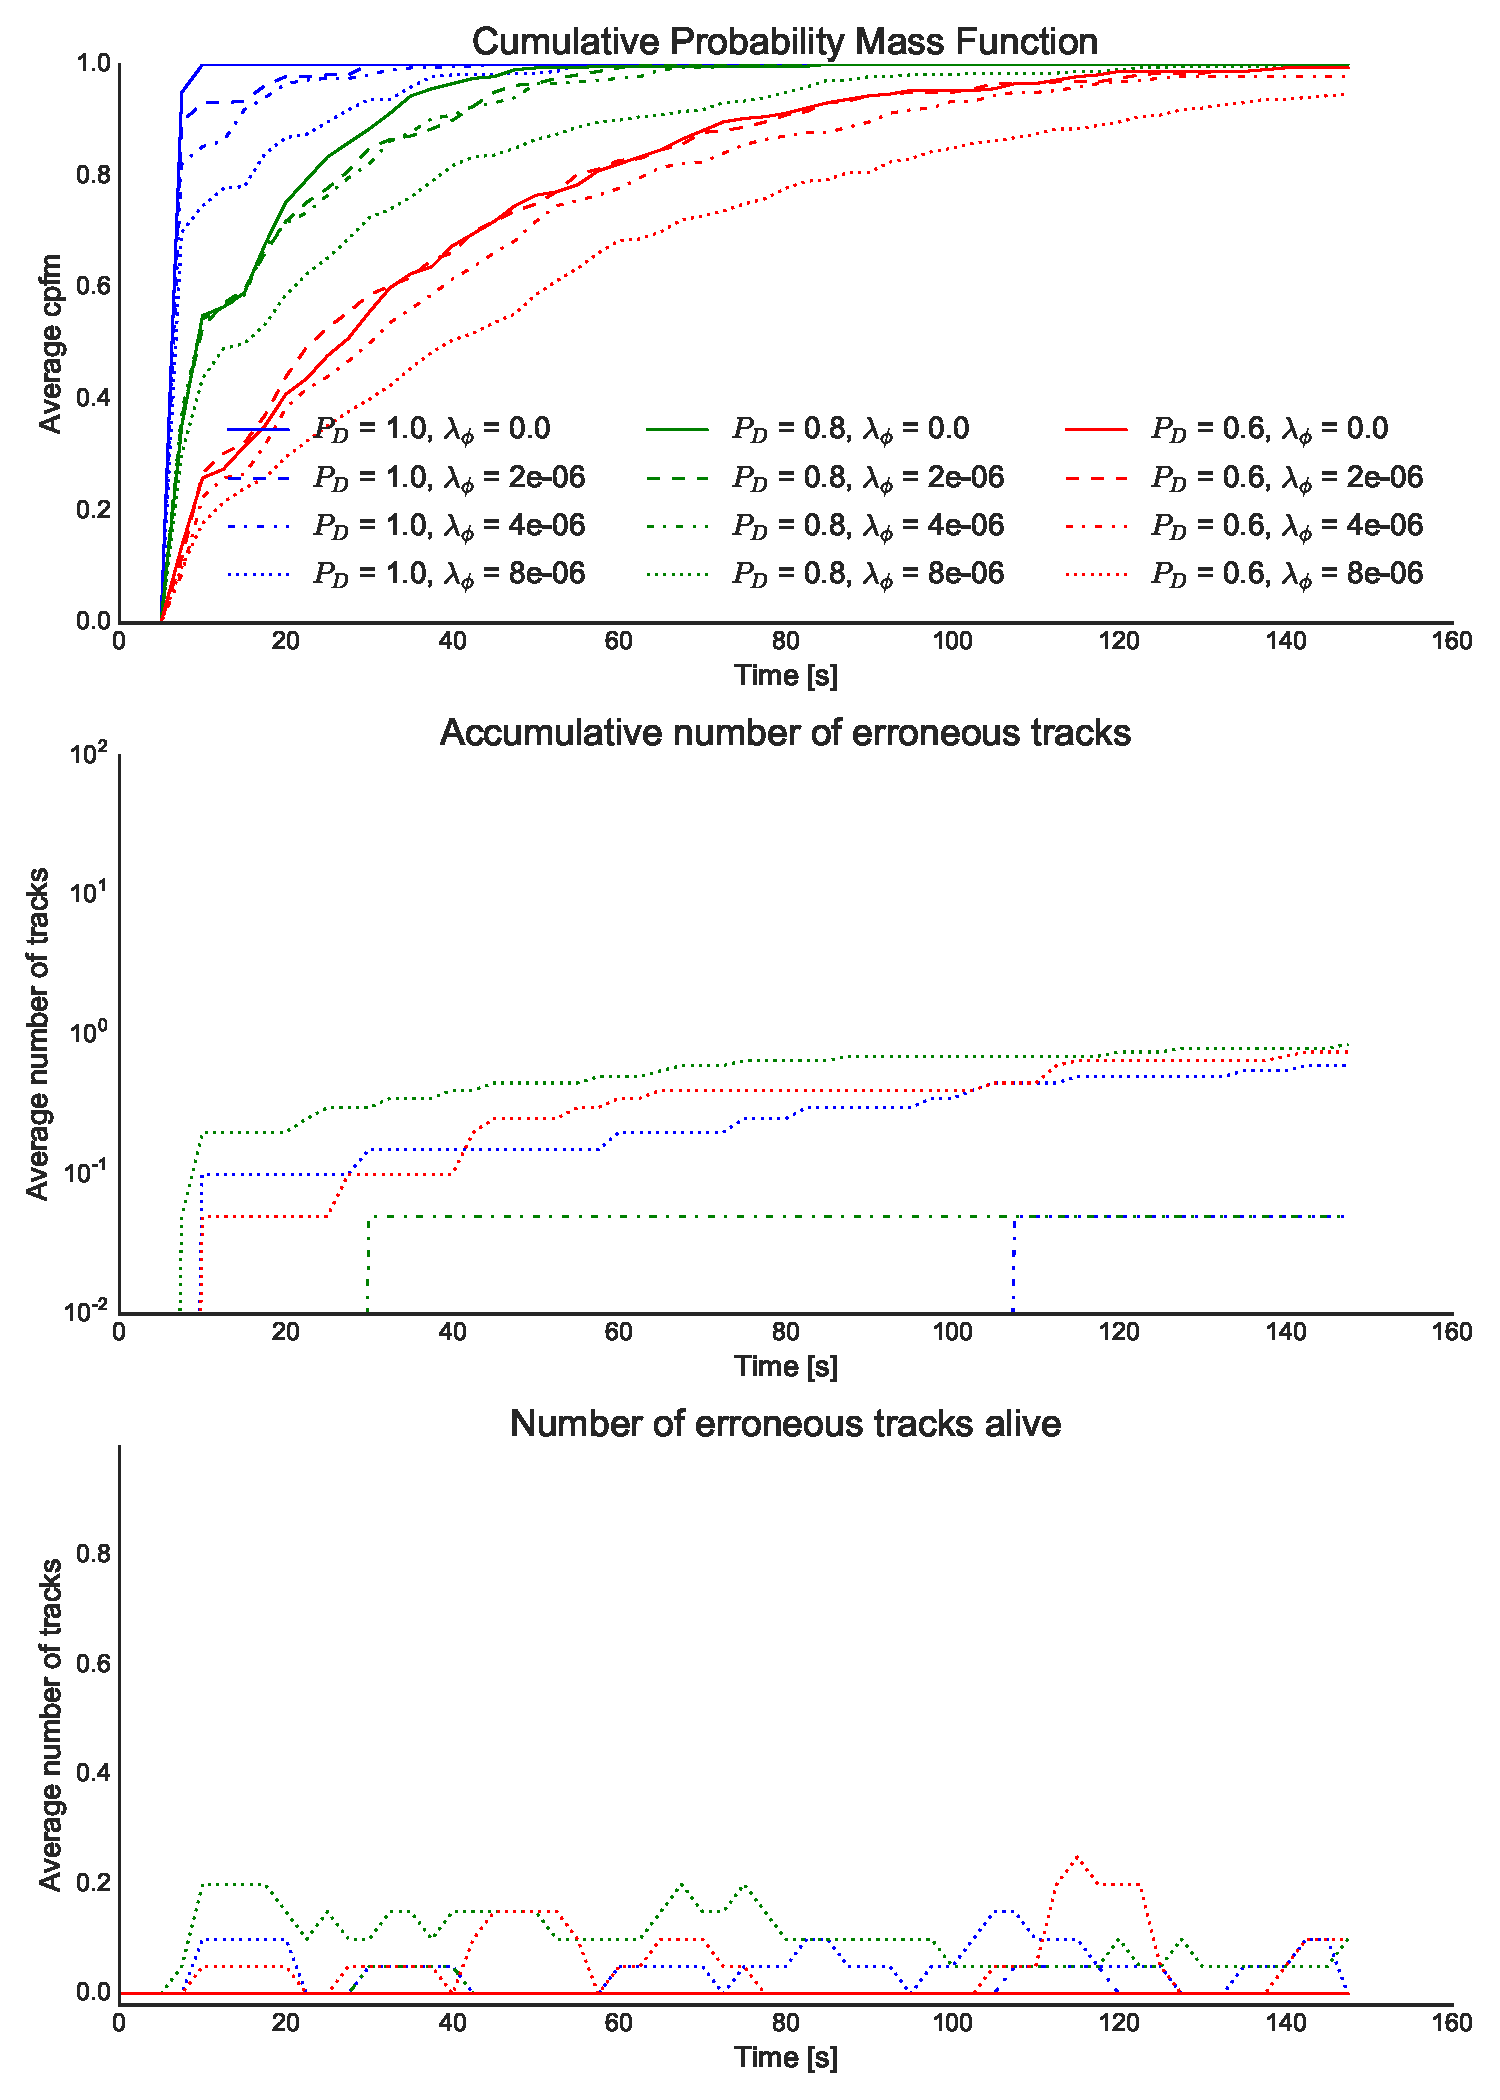
\includegraphics[height = .9\textheight]{Figures/plots/Scenario1_Init-Time(2-3).pdf}
\caption{Initialization time (2/3)}\label{fig:init_time_2-3}
\end{figure}

\begin{figure}
\centering
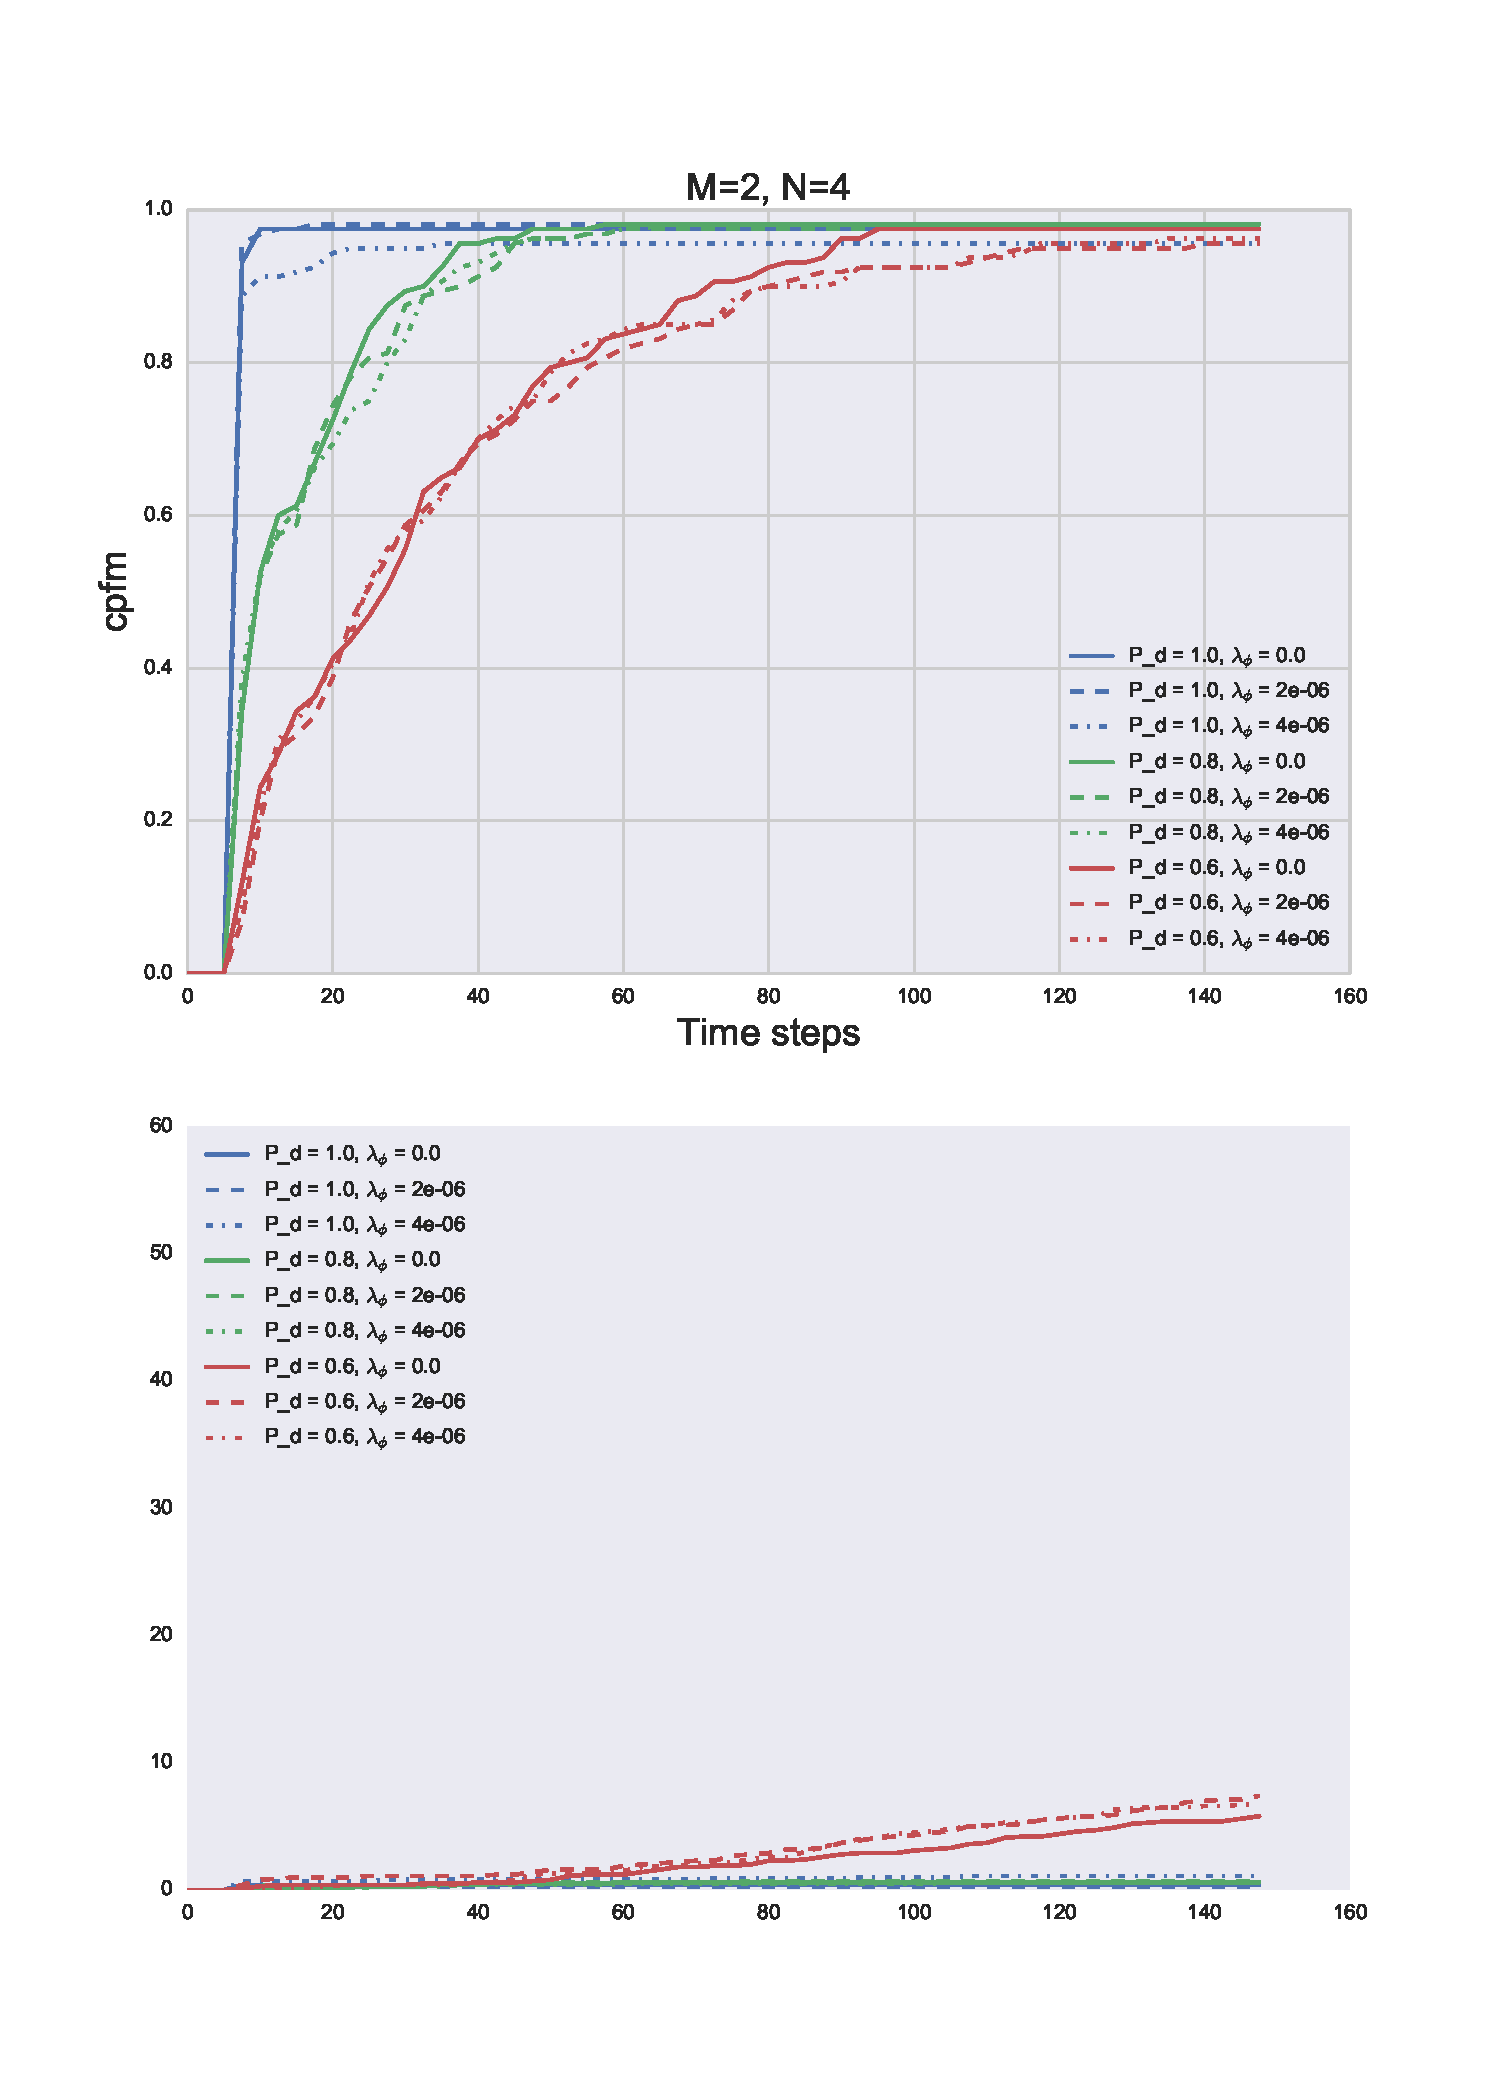
\includegraphics[height = .9\textheight]{Figures/plots/Scenario1_Init-Time(2-4).pdf}
\caption{Initialization time (2/4)}\label{fig:init_time_2-4}
\end{figure}

\begin{figure}
\centering
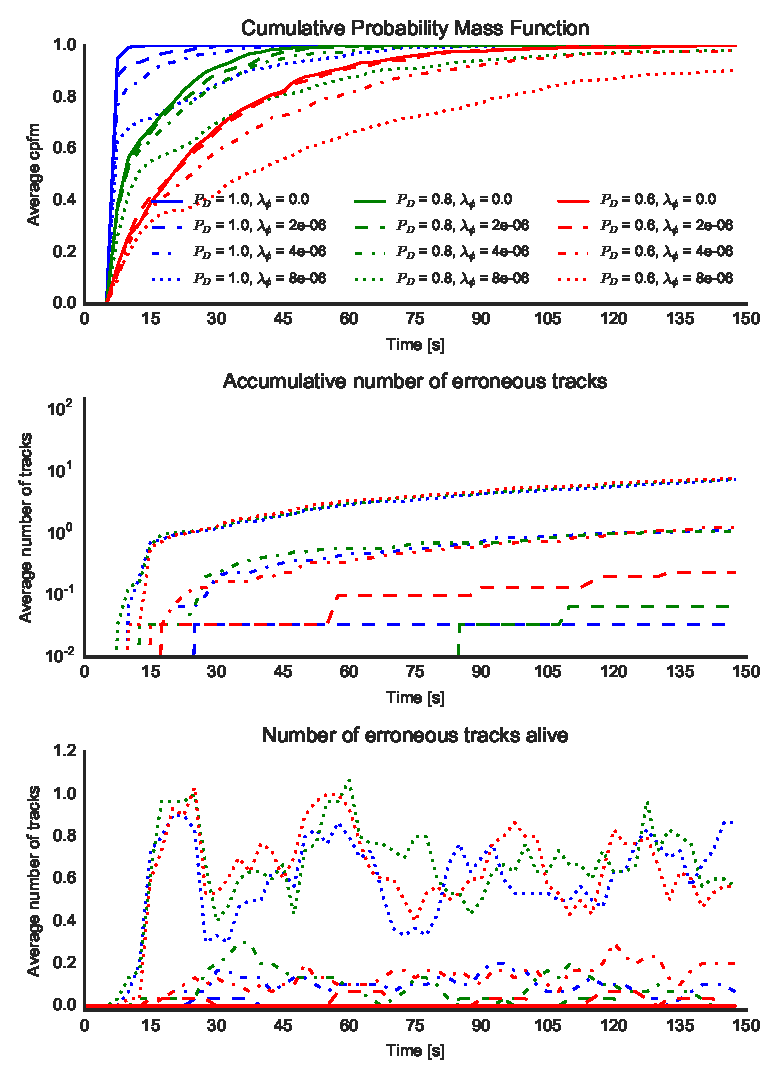
\includegraphics[height = .9\textheight]{Figures/plots/Scenario1_Init-Time(2-5).pdf}
\caption{Initialization time (2/5)}\label{fig:init_time_2-5}
\end{figure}

\begin{figure}
\centering
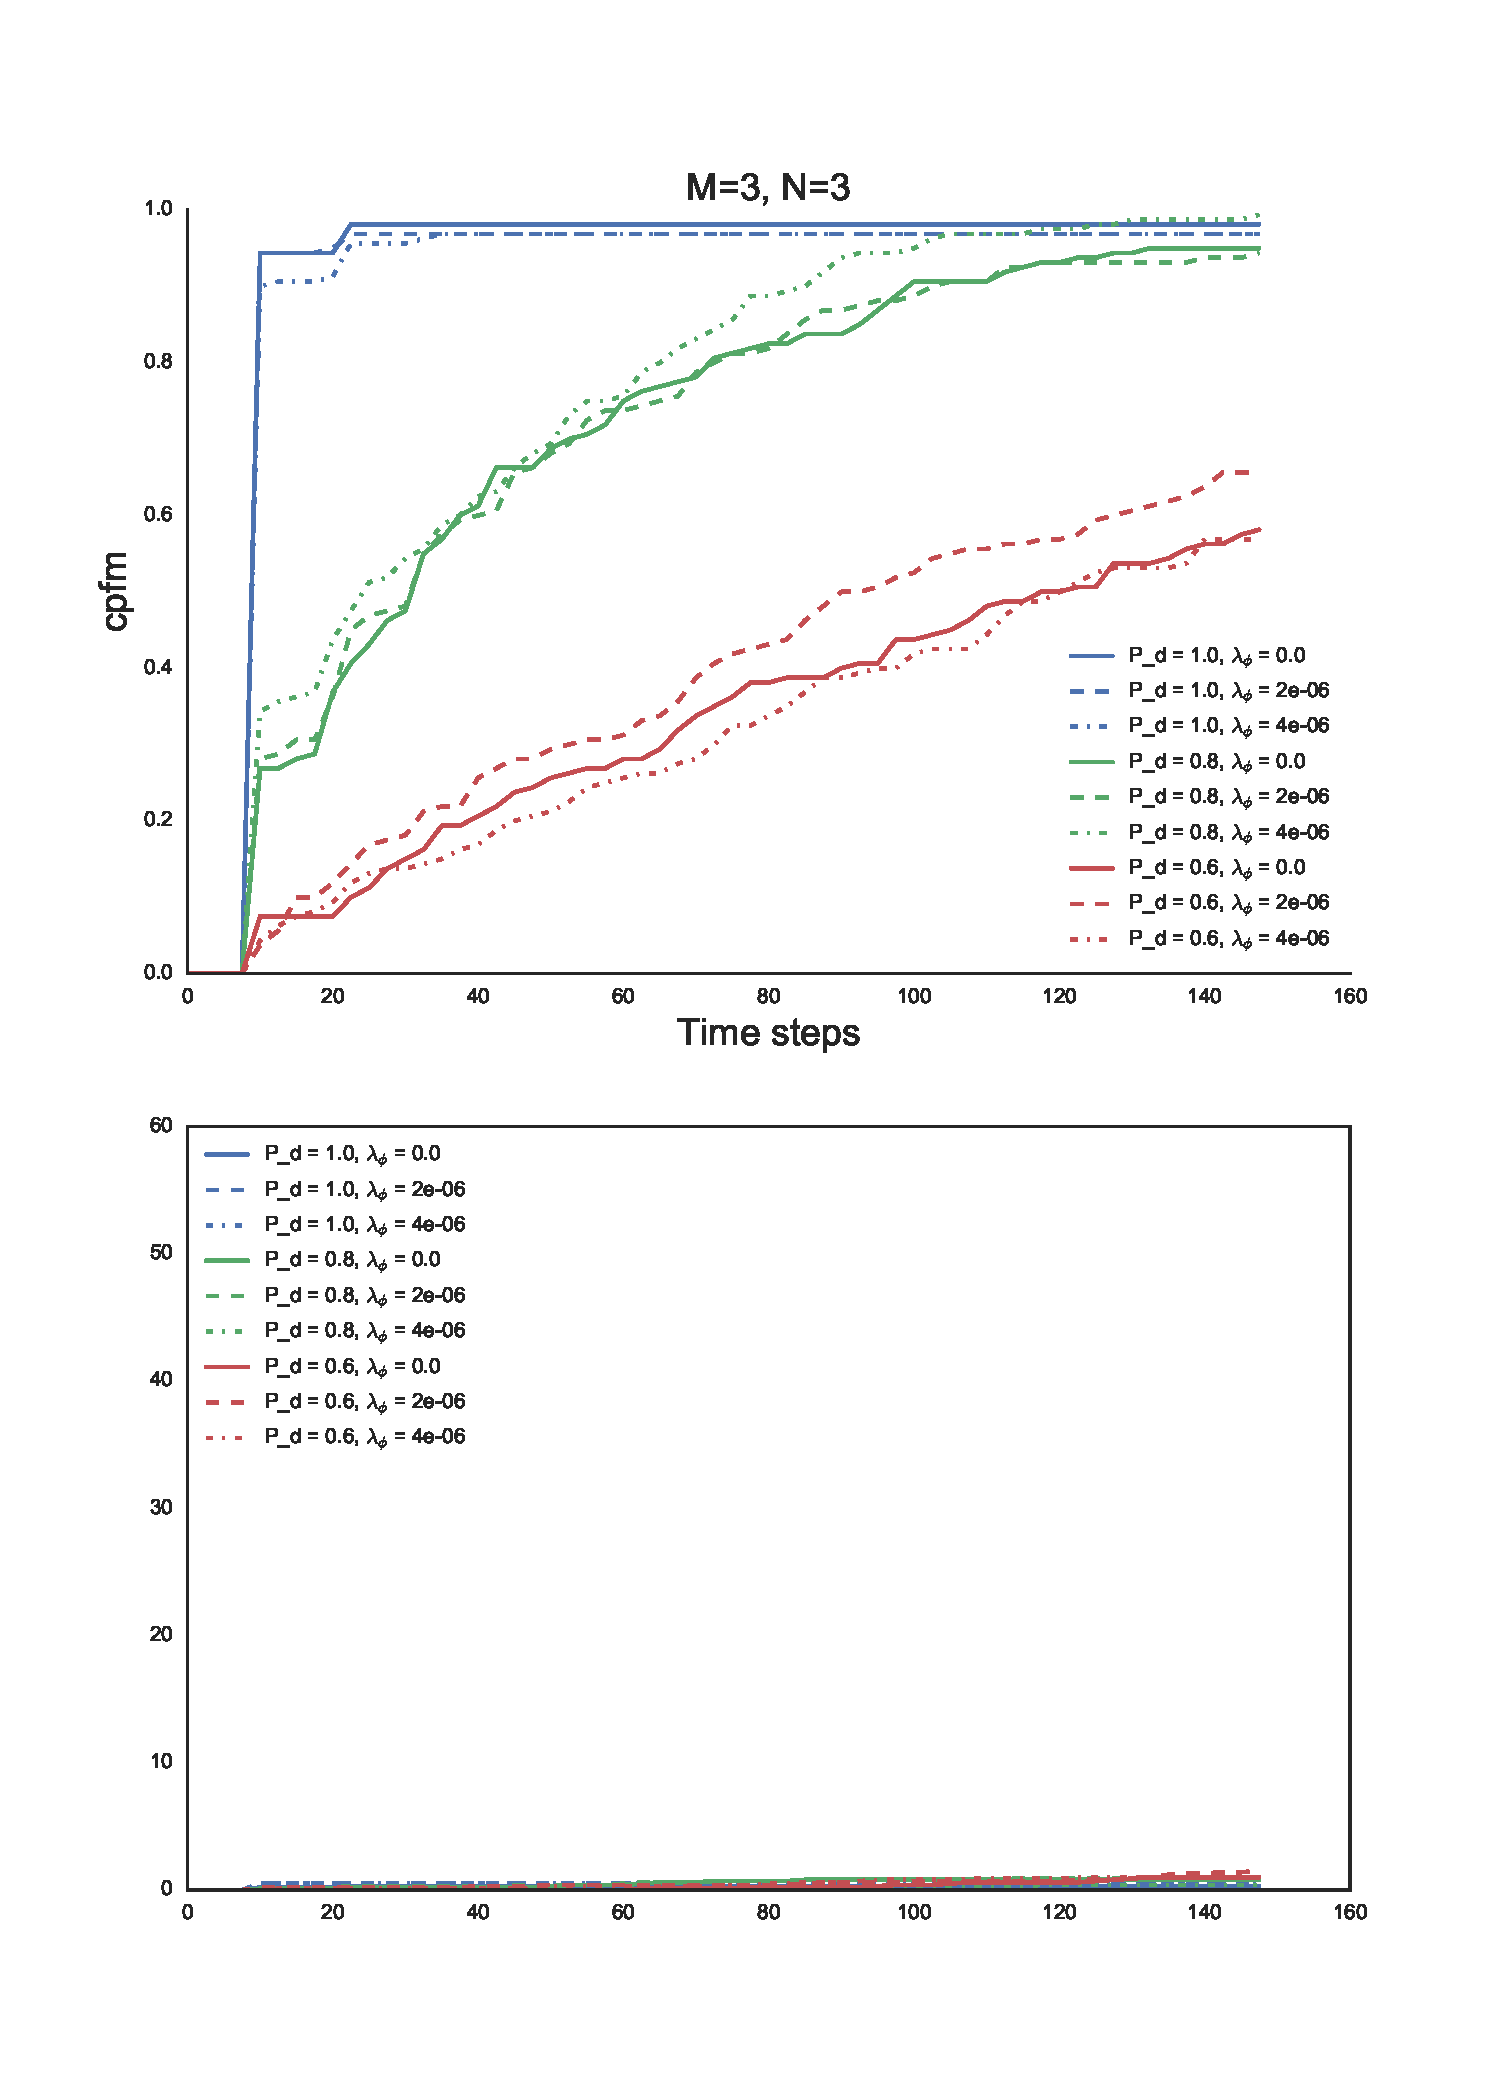
\includegraphics[height = .9\textheight]{Figures/plots/Scenario1_Init-Time(3-3).pdf}
\caption{Initialization time (3/3)}\label{fig:init_time_3-3}
\end{figure}

\begin{figure}
\centering
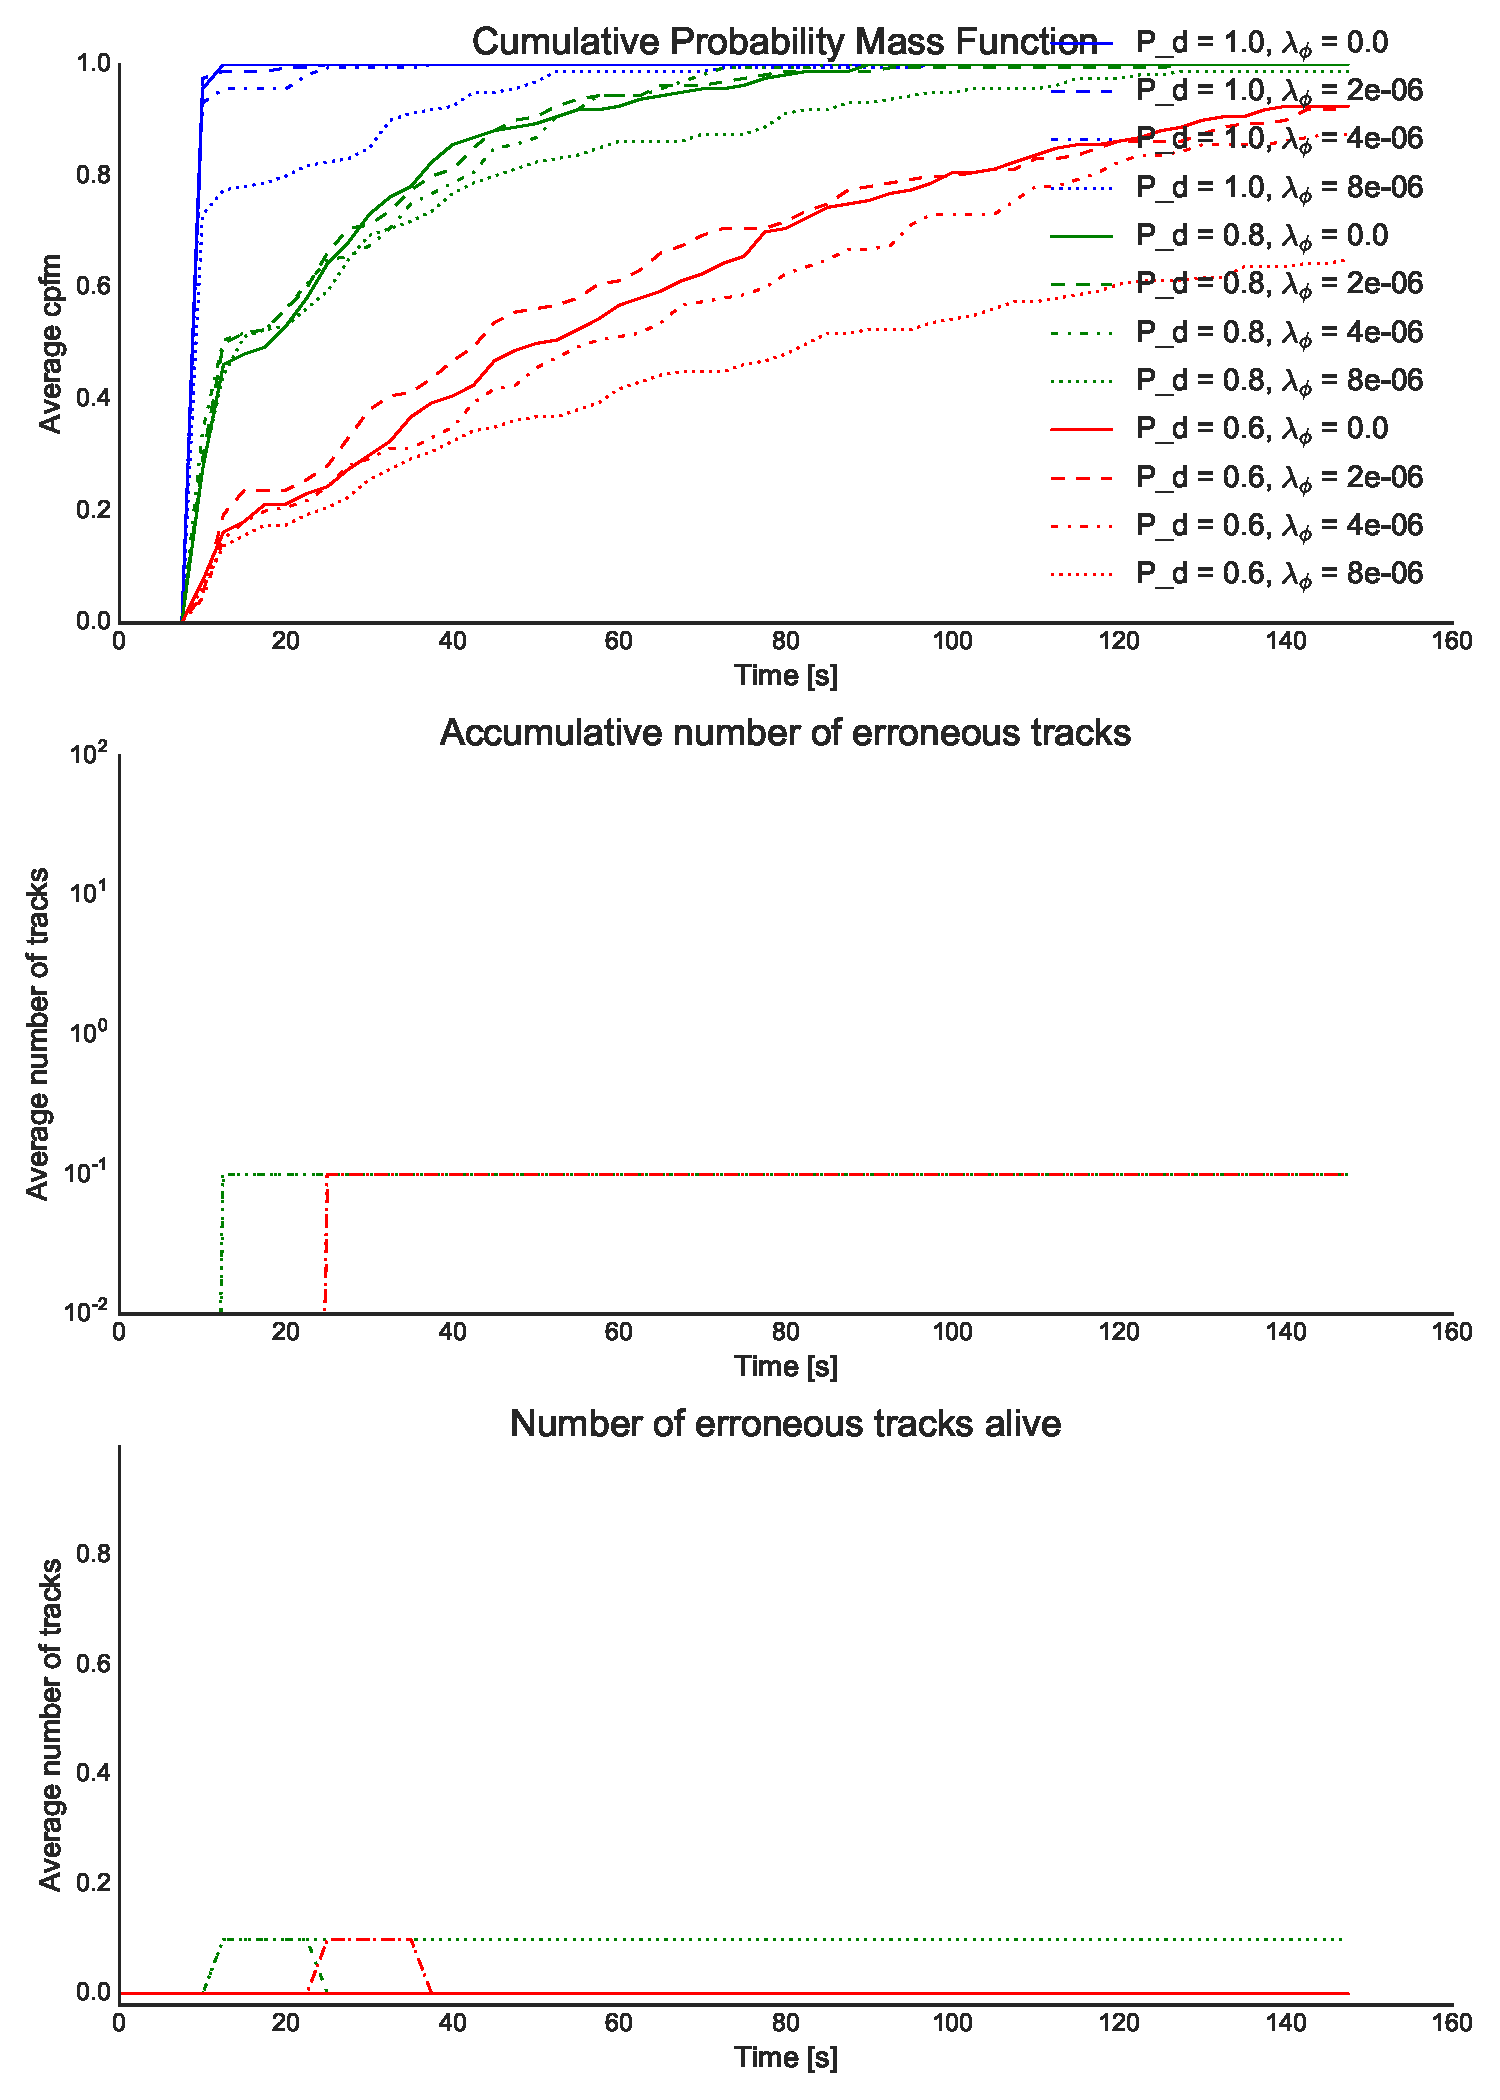
\includegraphics[height = .9\textheight]{Figures/plots/Scenario1_Init-Time(3-4).pdf}
\caption{Initialization time (3/4)}\label{fig:init_time_3-4}
\end{figure}

\begin{figure}
\centering
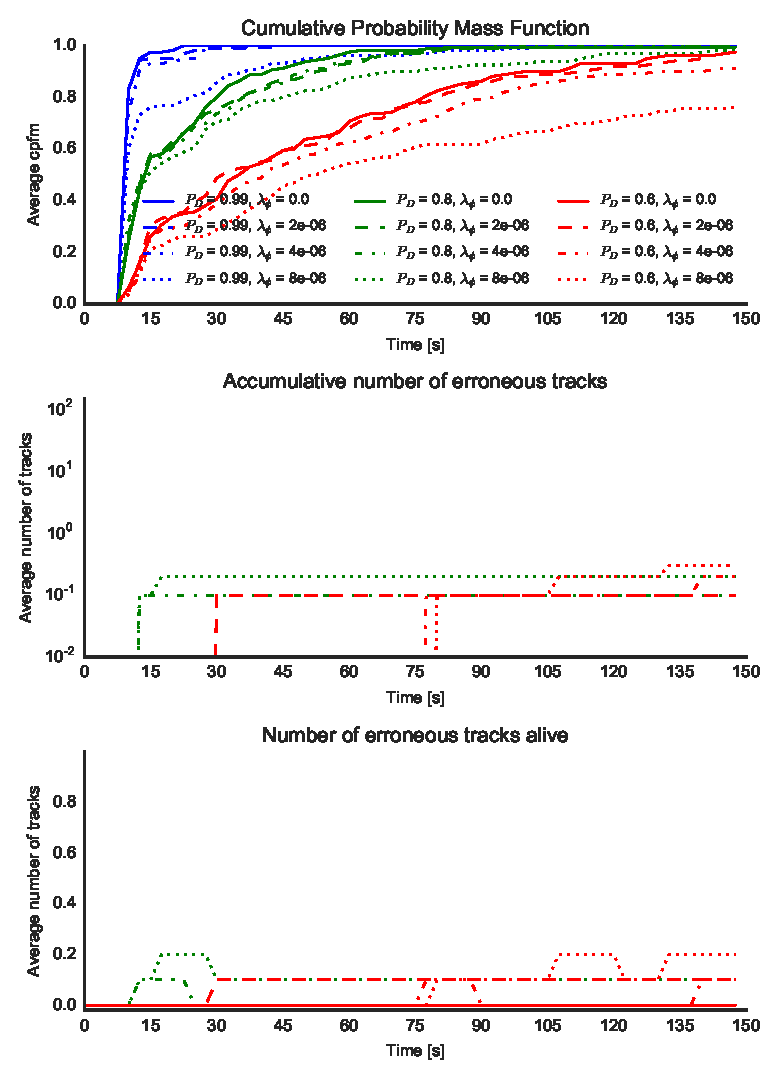
\includegraphics[height = .9\textheight]{Figures/plots/Scenario1_Init-Time(3-5).pdf}
\caption{Initialization time (3/5)}\label{fig:init_time_3-5}
\end{figure}

\begin{figure}
\centering
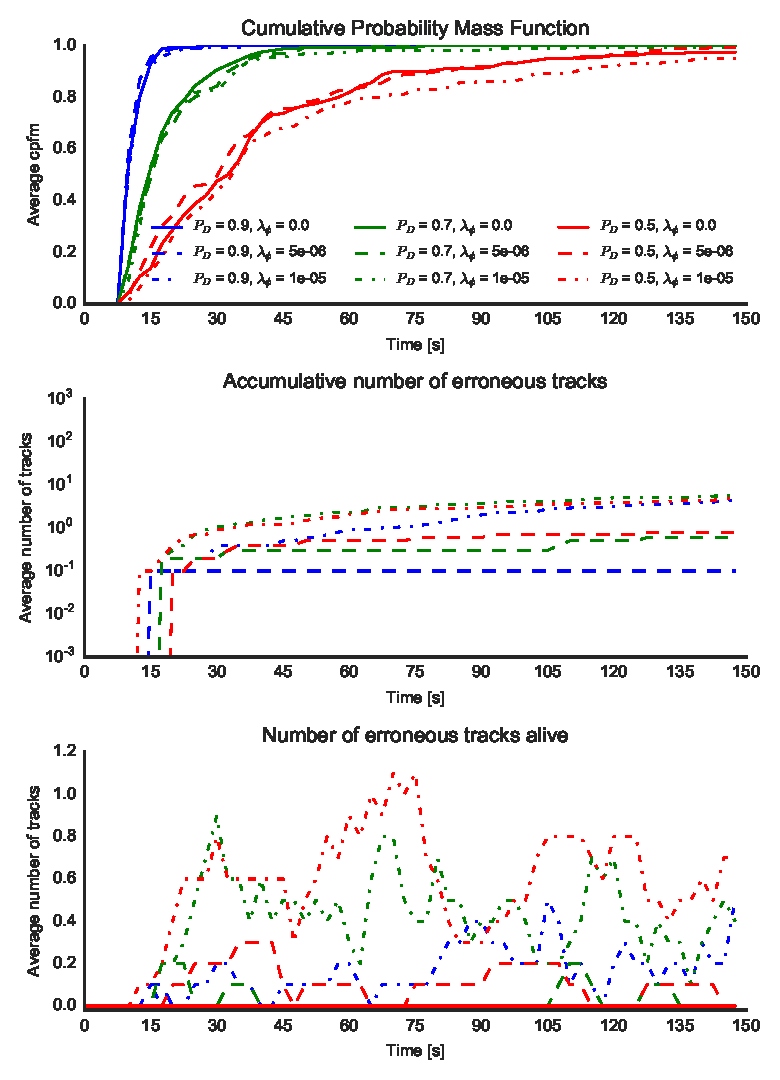
\includegraphics[height = .9\textheight]{Figures/plots/Scenario1_Init-Time(3-6).pdf}
\caption{Initialization time (3/6)}\label{fig:init_time_3-6}
\end{figure}
	%!TEX root = ../TTK4900-MHT.tex

\chapter{Track loss plot}
{
\setlength{\intextsep}{0mm}
\begin{figure}[H]
\centering
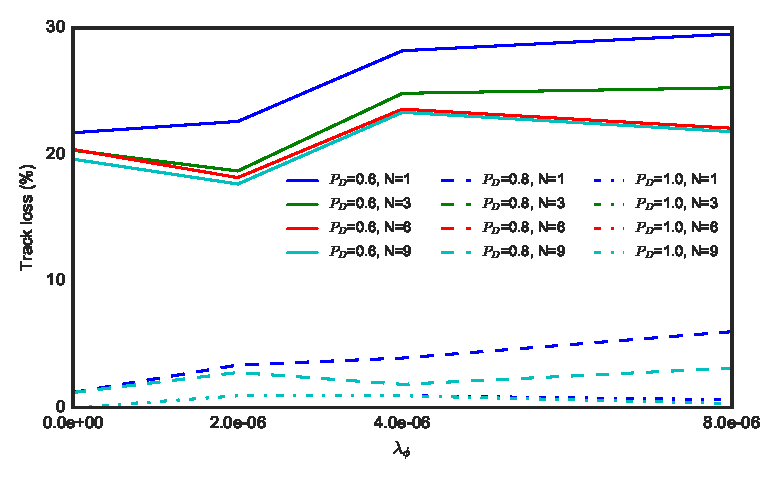
\includegraphics[height = .45\textheight]{Figures/plots/Scenario0_Tracking-TrackLoss.pdf}
\caption{Scenario 0 --- Track loss}\label{fig:scenario0_track_loss}
\end{figure}

\begin{figure}
\centering
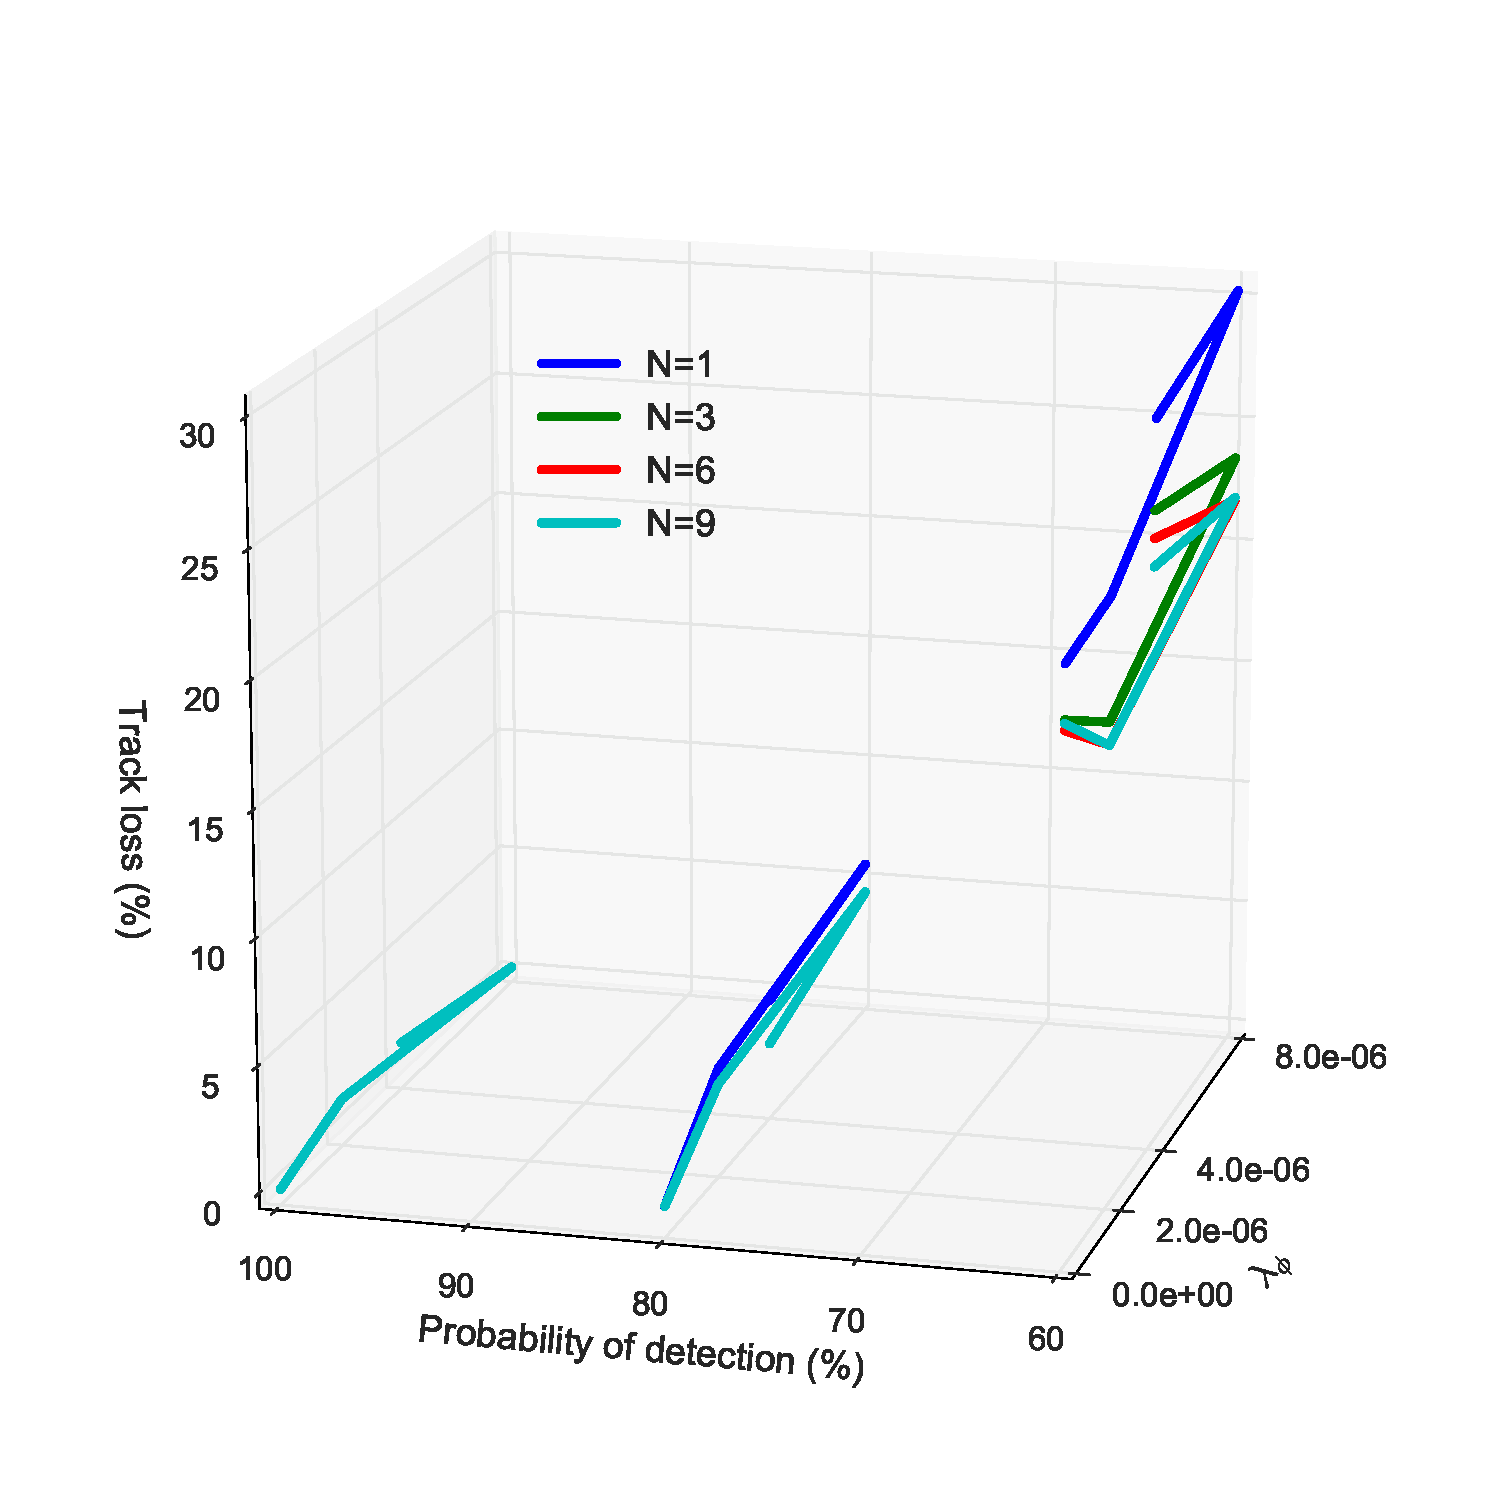
\includegraphics[height = .45\textheight]{Figures/plots/Scenario1_Tracking-TrackLoss.pdf}
\caption{Scenario 1 --- Track loss}\label{fig:scenario1_track_loss}

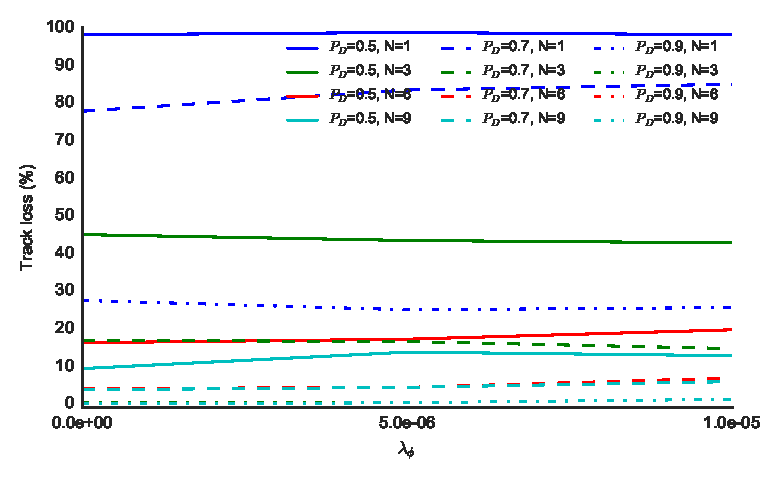
\includegraphics[height = .45\textheight]{Figures/plots/Scenario2_Tracking-TrackLoss.pdf}
\caption{Scenario 2 --- Track loss}\label{fig:scenario2_track_loss}
\end{figure}

\begin{figure}
\centering
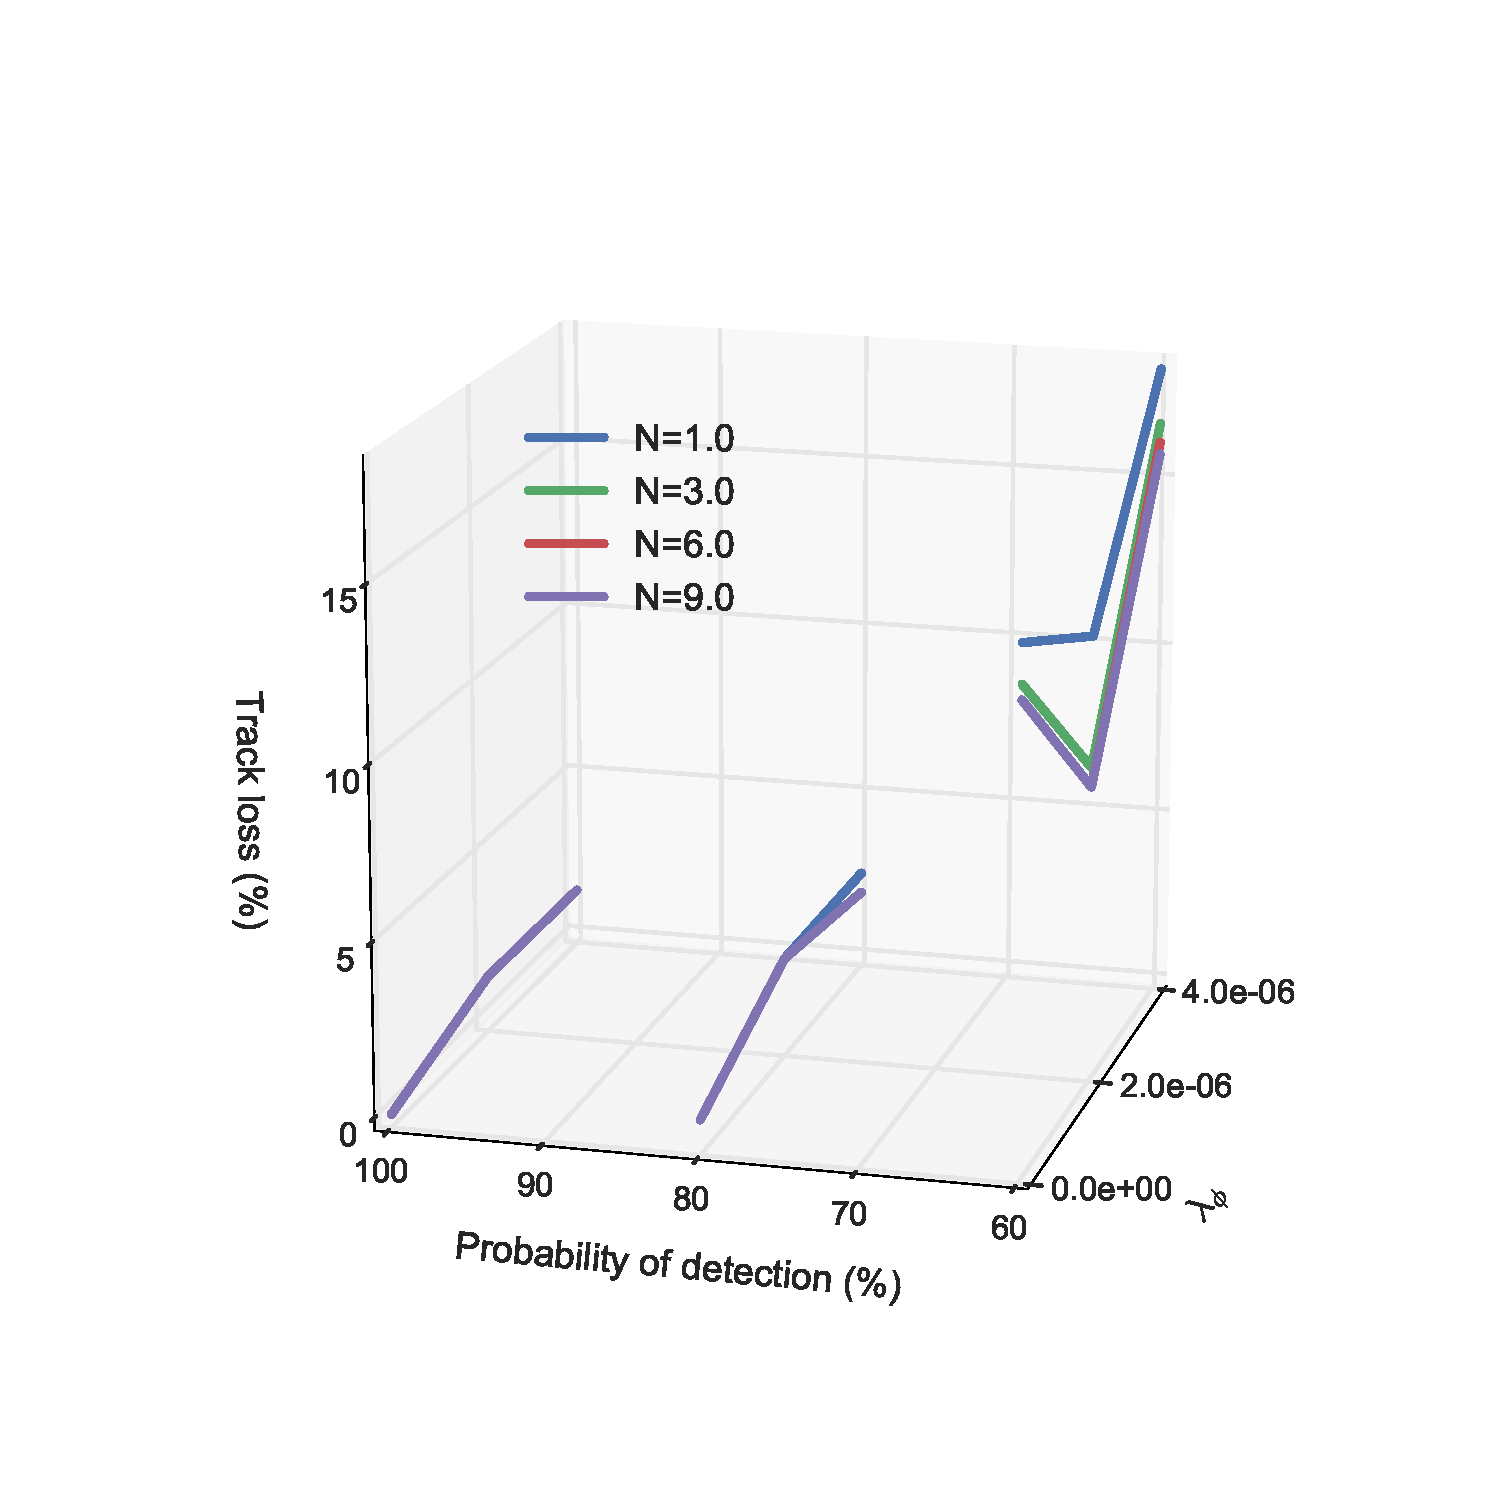
\includegraphics[height = .45\textheight]{Figures/plots/Scenario3_Tracking-TrackLoss.pdf}
\caption{Scenario 3 --- Track loss}\label{fig:scenario3_track_loss}

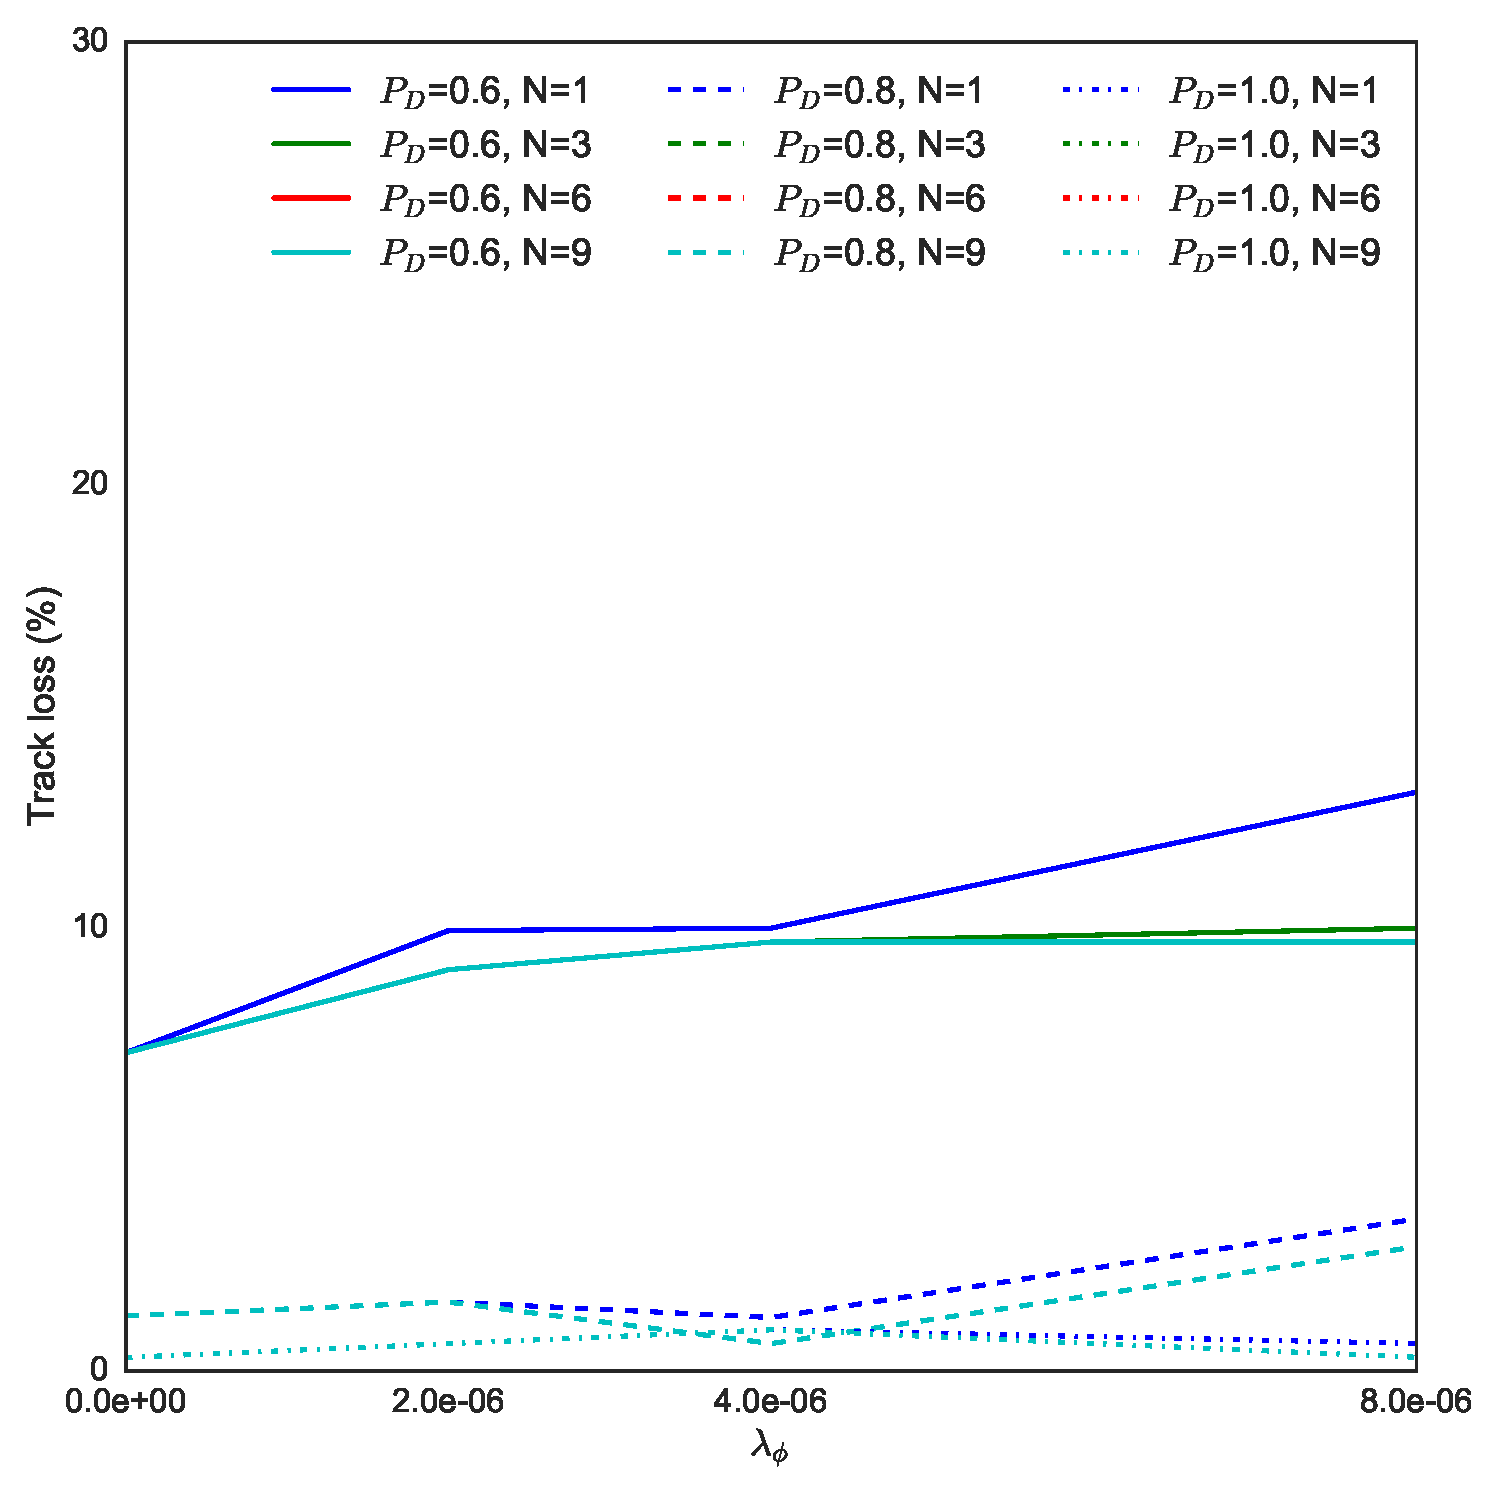
\includegraphics[height = .45\textheight]{Figures/plots/Scenario4_Tracking-TrackLoss.pdf}
\caption{Scenario 4 --- Track loss}\label{fig:scenario4_track_loss}
\end{figure}

}
	%!TEX root = ../TTK4900-MHT.tex

\chapter{Tracking percentage plot}
{
\setlength{\intextsep}{0mm}
\begin{figure}[H]
\centering
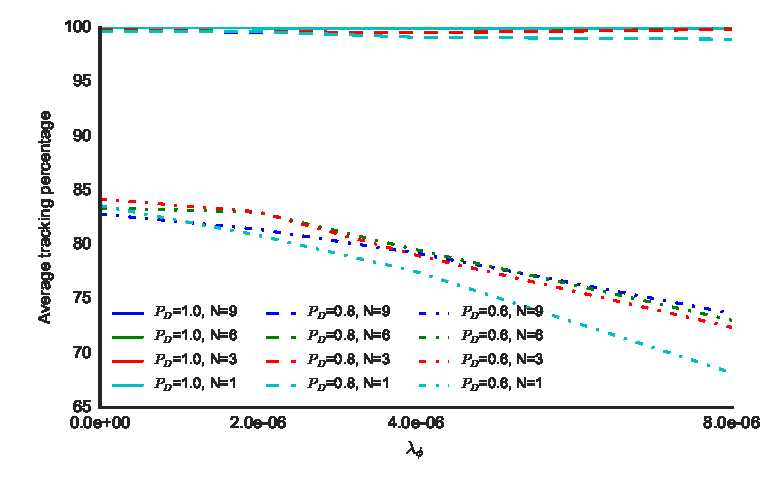
\includegraphics[height = .46\textheight]{Figures/plots/Scenario0_Tracking-TrackingPercentage.pdf}
\caption{Scenario 0 --- Tracking percentage}\label{fig:scenario0_tracking_percentage}
\end{figure}

\begin{figure}
\centering
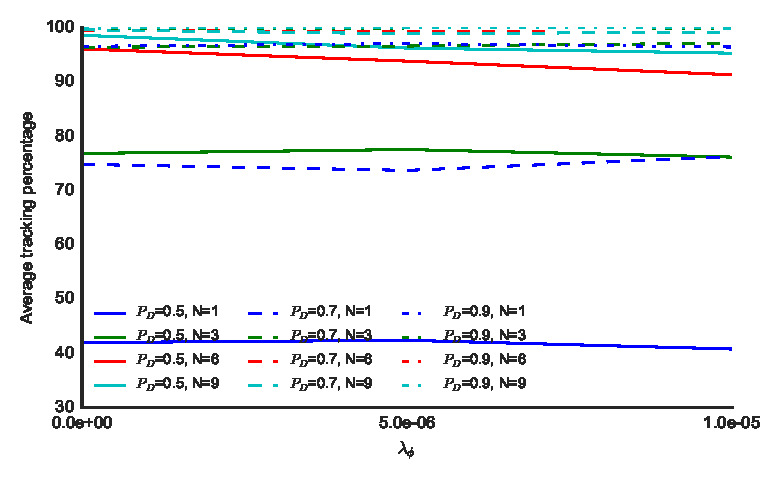
\includegraphics[height = .46\textheight]{Figures/plots/Scenario1_Tracking-TrackingPercentage.pdf}
\caption{Scenario 1 --- Tracking percentage}\label{fig:scenario1_tracking_percentage}

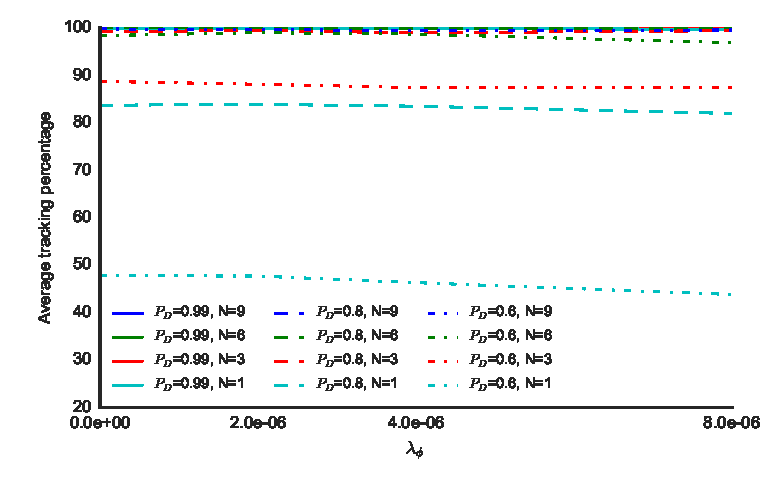
\includegraphics[height = .46\textheight]{Figures/plots/Scenario2_Tracking-TrackingPercentage.pdf}
\caption{Scenario 2 --- Tracking percentage}\label{fig:scenario2_tracking_percentage}
\end{figure}

\begin{figure}
\centering
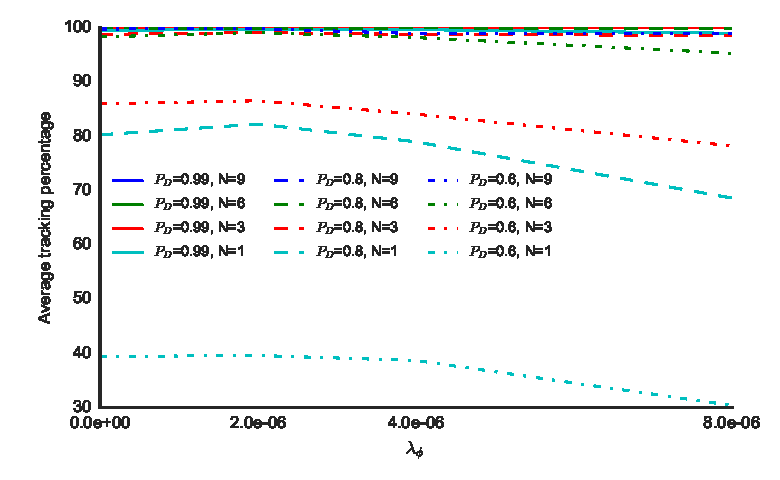
\includegraphics[height = .46\textheight]{Figures/plots/Scenario3_Tracking-TrackingPercentage.pdf}
\caption{Scenario 3 --- Tracking percentage}\label{fig:scenario3_tracking_percentage}

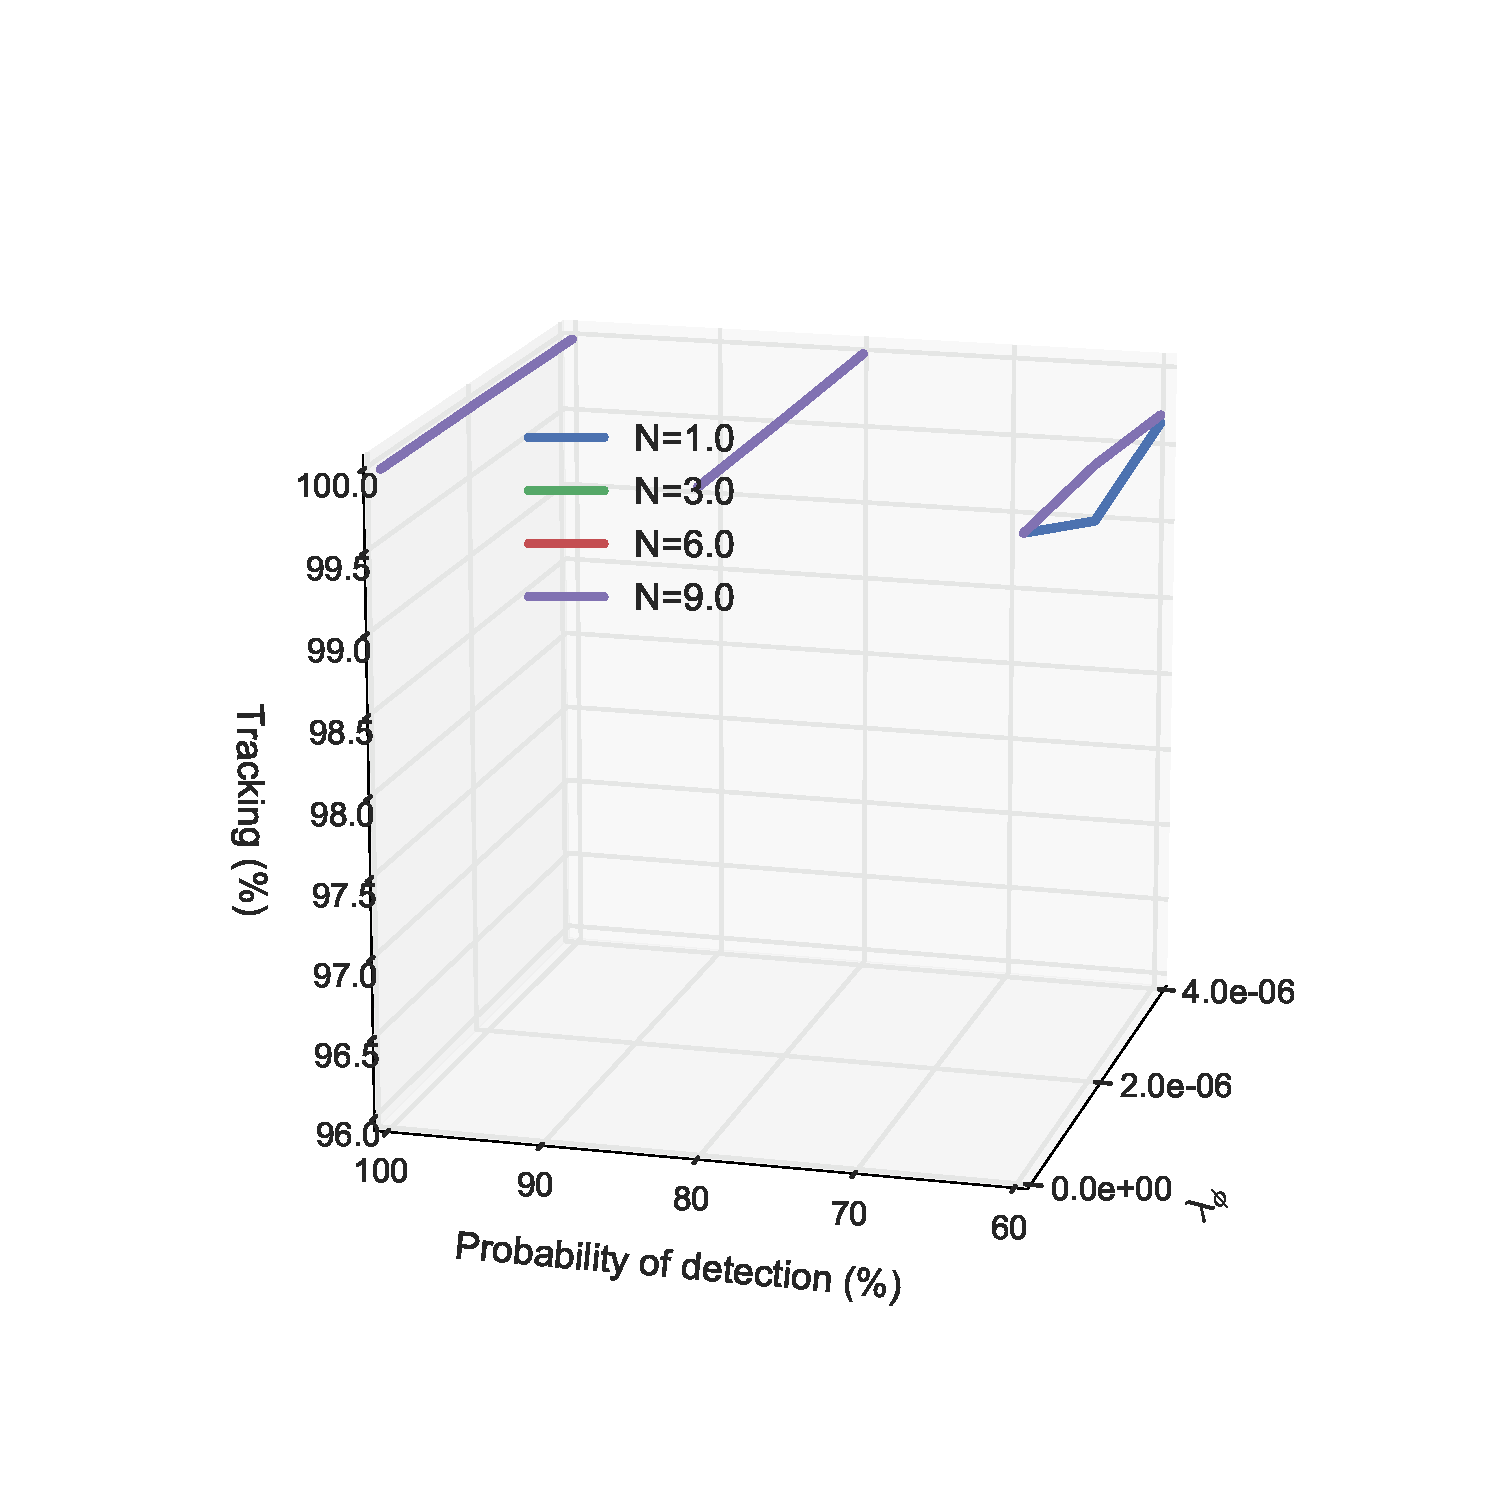
\includegraphics[height = .46\textheight]{Figures/plots/Scenario4_Tracking-TrackingPercentage.pdf}
\caption{Scenario 4 --- Tracking percentage}\label{fig:scenario4_tracking_percentage}
\end{figure}

}
\end{appendices} \clearpage %##Contains ArialMT type 3 linked fonts##
	\addcontentsline{toc}{chapter}{Bibliography}
	\printbibliography{}
\end{document}

%##Matplotlib PDF's contains ArialMT type 3 linked fonts##